%definira klasu dokumenta 
\documentclass[12pt]{report} 

%prostor izmedu naredbi \documentclass i \begin{document} se zove uvod. U njemu se nalaze naredbe koje se odnose na cijeli dokument

%osnovni LaTex ne može riješiti sve probleme, pa se koriste različiti paketi koji olakšavaju izradu željenog dokumenta
\usepackage[croatian]{babel} 
\usepackage{amssymb}
\usepackage{amsmath}
\usepackage{txfonts}
\usepackage{mathdots}
\usepackage{titlesec}
\usepackage{array}
\usepackage{lastpage}
\usepackage{etoolbox}
\usepackage{longtable, tabu}
\usepackage{color, colortbl}
\usepackage{adjustbox}
\usepackage{geometry}
\usepackage[classicReIm]{kpfonts}
\usepackage{hyperref}
\usepackage{fancyhdr}
\usepackage{ulem}

\usepackage{float}
\usepackage{setspace}
\restylefloat{table}


\patchcmd{\chapter}{\thispagestyle{plain}}{\thispagestyle{fancy}}{}{} %redefiniranje stila stranice u paketu fancyhdr

%oblik naslova poglavlja
\titleformat{\chapter}{\normalfont\huge\bfseries}{\thechapter.}{20pt}{\Huge}
\titlespacing{\chapter}{0pt}{0pt}{40pt}


\linespread{1.3} %razmak između redaka

\geometry{a4paper, left=1in, top=1in,}  %oblik stranice

\hypersetup{ colorlinks, citecolor=black, filecolor=black, linkcolor=black,	urlcolor=black }   %izgled poveznice


%prored smanjen između redaka u nabrajanjima i popisima
\newenvironment{packed_enum}{
	\begin{enumerate}
		\setlength{\itemsep}{0pt}
		\setlength{\parskip}{0pt}
		\setlength{\parsep}{0pt}
	}{\end{enumerate}}

\newenvironment{packed_item}{
	\begin{itemize}
		\setlength{\itemsep}{0pt}
		\setlength{\parskip}{0pt}
		\setlength{\parsep}{0pt}
	}{\end{itemize}}


%boja za privatni i udaljeni kljuc u tablicama
\definecolor{LightBlue}{rgb}{0.9,0.9,1}
\definecolor{LightGreen}{rgb}{0.9,1,0.9}


%podesavanje zaglavlja i podnožja

\pagestyle{fancy}
\lhead{Programsko inženjerstvo}
\rhead{Humanitarni šetači pasa}
\lfoot{Exception}
\cfoot{stranica \thepage/\pageref{LastPage}}
\rfoot{\today}
\renewcommand{\headrulewidth}{0.2pt}
\renewcommand{\footrulewidth}{0.2pt}


\begin{document} 
	
	
	
	\begin{titlepage}
		\begin{center}
			\vspace*{\stretch{1.0}} %u kombinaciji s ostalim \vspace naredbama definira razmak između redaka teksta
			\LARGE Programsko inženjerstvo\\
			\large Ak. god. 2020./2021.\\
			
			\vspace*{\stretch{3.0}}
			
			\huge dogGO\\
			\Large Dokumentacija, Rev. \textit{2}\\
			
			\vspace*{\stretch{12.0}}
			\normalsize
			Grupa: \textit{Exception}\\
			Voditelj: \textit{Eva Jagodić}\\
			
			
			\vspace*{\stretch{1.0}}
			Datum predaje: \textit{14.1.2021.}\\
	
			\vspace*{\stretch{4.0}}
			
			Nastavnik: \textit{Doria Bukić}\\
		
		\end{center}

	
	\end{titlepage}

	
	\tableofcontents

	\chapter{Dnevnik promjena dokumentacije}
		
		\begin{longtabu} to \textwidth {|X[2, l]|X[13, l]|X[3, l]|X[3, l]|}
			\hline \multicolumn{1}{|l|}{\textbf{Rev.}}	& \multicolumn{1}{l|}{\textbf{Opis promjene/dodatka}} & \multicolumn{1}{|l|}{\textbf{Autori}} & \multicolumn{1}{l|}{\textbf{Datum}} \\[3pt] \hline
			\endfirsthead
			
			\hline \multicolumn{1}{|l|}{\textbf{Rev.}}	& \multicolumn{1}{l|}{\textbf{Opis promjene/dodatka}} & \multicolumn{1}{|l|}{\textbf{Autori}} & \multicolumn{1}{l|}{\textbf{Datum}} \\[3pt] \hline
			\endhead
			
			\hline 
			\endlastfoot
			
			0.1 & Napravljen predložak.	& Jagodić & 15.10.2020. \\[3pt] \hline 
			0.2	& Dodan opis baze podataka. & Miletić & 26.10.2020. \\[3pt] \hline 
			0.3 & Dodan opis projektnog zadatka. & Smoljan & 28.10.2020. \\[3pt] \hline
			0.4 & Dodani funkcionalni i ostali zahtjevi te obrasci uporabe. & Pezo, Sentinella-Jerbić & 29.10.2020. \\[3pt] \hline 
			0.4.1 & Popravljeni funkcionalni zahtjevi. & Sentinella-Jerbić & 30.10.2020.  \\[3pt] \hline
			0.5 & Dodan uvod u arhitekturu i dizajn sustava. & Sentinella-Jerbić & 6.11.2020.  \\[3pt] \hline
			0.6 & Dodani dijagrami obrazaca uporabe & Jagodić & 9.11.2020.  \\[3pt] \hline
			0.7 & Dodani sekvencijski dijagrami & Golub, Miletić & 10.11.2020.  \\[3pt] \hline
			0.8 &  Dodana prva verzija dijagrama razreda. & Sentinella-Jerbić & 11.11.2020. \\[3pt] \hline
			0.8.1 & Popravci dijagrama razreda. & Golub, Sentinella-Jerbić & 11.11.2020. \\[3pt] \hline
			\textbf{1.0} & Verzija samo s bitnim dijelovima za 1. ciklus & Jagodić & 13.11.2020. \\[3pt] \hline 
			1.1 & Dodane korištene tehnologije i alati  & Sentinella-Jerbić & 12.1.2021. \\[3pt] \hline
			1.2 & Dodani dijagrami stanja  & Pezo & 12.1.2021. \\[3pt] \hline
			1.3 & Dodani dijagrami aktivnosti i razmještaja  & Terović & 12.1.2021. \\[3pt] \hline
			1.4 & Ispitivanje programskog rješenja & Golub, Miletić & 14.1.2021. \\[3pt] \hline
			1.5 & Zaključak i budući rad & Jagodić & 14.1.2021. \\[3pt] \hline
			1.6 & Dodan dijagram komponenti & Smoljan & 14.1.2021 \\[3pt] \hline
			1.7 & Ažurirani dijagrami razreda & Sentinella-Jerbić & 14.1.2021 \\[3pt] \hline
			1.8 & Dodane upute za puštanje u pogon & Smoljan & 14.1.2021 \\[3pt] \hline
			\textbf{2.0} & Konačni tekst predloška dokumentacije  & Jagodić & 14.1.2021. \\[3pt]
		\end{longtabu}
	\chapter{Opis projektnog zadatka}

    \section{Motivacija i osnovna ideja}
    
        Broj napuštenih pasa u skloništima u Hrvatskoj, pa i ostalim europskim zemljama, svaki dan je sve veći i veći. Kao posljedica toga, psi u prosjeku provode sve više vremena u skloništu čekajući svog novog vlasnika. S druge strane, postoje brojni ljudi koji vole pse i žele im pomoći, ali nisu u mogućnosti udomiti psa, bilo zbog manjka prostora ili nedostatka vremena. \newline \\
        Jedan od najboljih načina na koji mogu pomoći, a da ne udome psa, je šetnjama. Tako se psima olakšava čekanje i smanjuje vrijeme provedeno u skloništu, te ga se ispunjava na koristan način – fizičkom aktivnošću i socijalizacijom.
        Ljudima se pruža prilika da uživaju u druženju sa psima, a možda da upoznaju i svog novog najboljeg prijatelja. \newline \\
        Kako je većina ljudi vrlo zaposlena ideja je stvoriti web aplikaciju koja bi na jednostavan i brz način spojila udruge za zaštitu životinja i zainteresirane građane-šetače pasa. Olakšavanjem postupka same prijave za šetnju i kreiranjem atraktivne aplikacije koja je lagana za korištenje, smatramo da bi se znatno povećao broj zainteresiranih građana. \newline \\
        Aplikacija je namijenjena dvjema skupinama krajnjih korisnika: građanima - potencijalnim šetačima pasa i udrugama za zaštitu životinja. \newline \\
        Prijavom u sustav udruge unose podatke o psima koje žele uključiti u aktivnost. Građani zatim mogu pregledati sve udruge i pse raspoložive za šetnju, te odabrati psa i rezervirati termin šetnje. Odabrani termin vidljiv je udruzi koja u dogovoreno vrijeme predaje psa šetaču. Aplikacija također vodi statistiku o svim provedenim šetnjama te ju, uz korisnikovu suglasnost, prikazuje javno u obliku rang liste najaktivnijih šetača.
        
    \section{Detaljan opis rješenja}
        \subsection{Općenito}
        
        Glavna namjena aplikacije je spajanje ljubitelja životinja s udrugama kojima je njihova pomoć, u vidu šetnji, potrebna. Aplikacija bi bila realizirana kao web aplikacija, uključujući i prilagodbu za prikaz na mobilnim uređajima. Bila bi dostupna na području države, te potencijalno korištena od strane većeg broja korisnika (pregledi zainteresiranih građana).
    
    \subsection{Vrste korisnika}
    
        Korisnik je svaka osoba, ne nužno registrirana, koja u bilo kojem trenutku pregledava ili koristi neki dio aplikacije. Razlikujemo dva tipa korisnika: šetače i udruge.
        \begin{packed_item}
            \item[1)] \textbf{Građani - šetači} \\
            Pod šetače spadaju svi korisnici koji aplikaciju upotrebljavaju s ciljem pronalaska psa za šetnju. Razlikujemo neregistrirane korisnike (javni posjetitelji) te registrirane korisnike.
            \begin{packed_item}
                        \item[a)] \textbf{Neregistrirani korisnici (javni posjetitelji)}\\
                        Jedan od glavnih ciljeva aplikacije je zainteresirati što veći broj ljudi za šetanje pasa. Stoga i neregistrirani korisnici imaju mogućnost pregleda profila svih udruga, profila njihovih pasa koji sudjeluju u programu, pregled statistika šetnje svih pasa unutar neke udruge te lokaciju same udruge. Statistika šetnji također nudi informacije o psima koji su manje šetani od ostalih te koji imaju veću potrebu za šetnjom. Korisniku se nudi i opcija prijave za šetanje pasa, a ako korisnik odabere tu opciju, korisnika se obavještava da kako bi napravio registraciju treba biti prijavljen u sustav.
            
                        \item[b)] \textbf{Registrirani korisnici} \\
                        Kako bi se korisnik registrirao za šetača, mora navesti:
                        \begin{packed_item}
                            \item[$\bullet$] ime
                            \item[$\bullet$] prezime
                            \item[$\bullet$] adresu e-pošte
                            \item[$\bullet$] željeno korisničko ime
                            \item[$\bullet$] lozinku
                        \end{packed_item}
                        
                        Nakon što korisnik obavi registraciju, ima opciju pregleda udruga i pasa raspoloživih za šetnju, isto kao i neregistrirani korisnik. Međutim, kao registriranom korisniku pružaju mu se i mogućnosti odabira psa za šetnju, odabir željenog termina te prijava za samu šetnju.  Nakon odabira termina šetnje, bilo javne ili grupne, korisniku se termin šetnje prikazuje u kalendaru, a svoj raspored može preuzeti i u PDF obliku.
                        Također, svi registrirani korisnici imaju opciju pregleda vlastitog profila, uključujući nadolazeće i prethodne šetnje, statistike, osobne podatke i slično. Mogu označiti vlastite statistike šetnji kao javne, u kojem slučaju se one mogu pojaviti na javnoj rang listi.
                        Imaju i opciju uređivanja svojih podataka, te brisanja računa na stranici.
            \end{packed_item}
            
            \item[2)] \textbf{Udruge} \\
                Kako bi se obavila registracija, udruga mora navesti:
                \begin{packed_item}
                    \item[$\bullet$] ime i prezime osobe koja predstavlja udrugu
                    \item[$\bullet$] adresu e-pošte
                    \item[$\bullet$] naziv udruge
                    \item[$\bullet$] OIB udruge
                    \item[$\bullet$] željeno korisničko ime
                    \item[$\bullet$] lozinku
                \end{packed_item}
                Nakon obavljene prijave, udruga može započeti sa stvaranjem profila za pse u svojem skrbništvu.
                \newline
                Za stvaranje profila jednog psa, udruga navodi sljedeće informacije:
                \begin{enumerate}
                    \item[$\bullet$] ime
                    \item[$\bullet$] slika (neobavezno)
                    \item[$\bullet$] opis psa
                    \item[$\bullet$] preferirani način šetnje
                        \begin{enumerate}
                            \item[$\bullet$] invidualna šetnja / šetnja s drugim psima
                        \end{enumerate}
                    \item[$\bullet$] vrsta
                \end{enumerate}
                Ti profili, zajedno sa osnovnim informacijama o udruzi te statistikama šetnji svih njenih pasa, javno su dostupni svim korisnicima web aplikacije. Udruga u bilo kojem trenutku može obrisati neki od profila pasa , u kojem slučaju se otkazuju i svi budući termini šetnji na koje je prijavljen. \newline \\
                Udruga također ima pristup svim rezervacijama za svoje pse, koje imaju opciju otkazati. \newline \\
                Udruga također ima opciju pregleda svojih podataka i uređivanja istih, kao i brisanja svog profila iz aplikacije. U tom slučaju se automatski brišu i profili svih pasa registriranih preko te udruge.
        \end{packed_item}
        \section{Opis funkcionalnosti aplikacije}
        \subsection{Pregled pasa / udruga}
        
            Ovo je jedna od glavnih funkcionalnost aplikacije. I registriranim i neregistriranim korisnicima omogućen je prikaz svih pasa koji sudjeluju u programu, te je omogućeno i filtriranje pasa prema lokaciji, udruzi, preferiranom načinu šetnje itd. Moguć je i pregled profila svih udruga, te pojedinih pasa o kojima neka udruga skrbi (a koji sudjeluju u programu) . \\
            
            \noindent Profil psa sadrži kratke informacije o psu, kao i njegovu sliku te termine u kalendaru i točno vrijeme kada je pas dostupan za šetnju. 
        
        \subsection{Rezervacija i potvrda termina šetnje}
        
            Nakon što korisnik pronađe psa kojeg želi šetati, sljedeći korak je rezervacija termina šetnje. Korisnik prvo pregledava termine u kalendaru kada je pas dostupan, te odabire termin koji mu odgovara. Ukoliko je korisnik odabrao psa koji voli grupne šetnje, tada korisnik u istom terminu može odabrati još jednog psa koji voli grupne šetnje, pod uvjetom da su iz iste udruge.

            
        \subsection{Pregled statistika}
        Postojio nekoliko vrsta statistike koje aplikacija vodi:
            \begin{enumerate}
                \item \textbf{Statistike šetača pasa}
                    \begin{enumerate}
                        \item[$\bullet$] uključuju broj šetnji, broj prošetanih pasa te ukupnu duljinu šetnji
                        \item[$\bullet$] po defaultu privatna statistika, korisnik ju sam može učiniti javnom, u kojem slučaju se prikazuje i na naslovnoj stranici, u sklopu liste najaktivnijih šetača
                    \end{enumerate}
                
                \item \textbf{Statistike udruge}
                    \begin{enumerate}
                        \item[$\bullet$] uključuje broj pasa u skrbi udruge te ukupan broj šetnji obavljen sa psima udruge
                        \item[$\bullet$] statistika javno dostupna svim korisnicima
                    \end{enumerate}
                    
                \item \textbf{Statistike admina}
                    \begin{enumerate}
                        \item[$\bullet$] ukupan broj aktivnih korisnika stranice
                        \item[$\bullet$] ukupan broj aktivnih udruga na stranici
                        \item[$\bullet$] ukupan broj pasa uključenih u program stranice
                    \end{enumerate}
            \end{enumerate}
        
    \section{Implementacijski detalji}
        Kako je jedan od glavnih ciljeva aplikacije privući što više korisnika u program, aplikacija mora podržavati istovremeni rad većeg broja korisnika. Za implementaciju backend dijela aplikacije odabran je programski jezik Java, uz pomoć frameworka Spring, dok je za frontend korišten React.\\
        
        \noindent Aplikacija se krajnim korisnicima prikazuje u obliku web-stranice, prilagođene za prikaz na mobilnim uređajima kao i na osobnim računalima.
        
    \section{Pregled konkurentskih rješenja i stanje tržišta}
    
        Najbliže konkurentske aplikacije su aplikacije za plaćeno šetanje pasa, poput BarkleyPets ( \url{https://barklypets.com/}), WagWalking(\url{https://wagwalking.com/}), DogHero (\url{https://play.google.com/store/apps/details?id=br.com.doghero.astro}) i slično. Iako ove aplikacije predstavljaju određenu konkurenciju, u smislu da ciljaju istu skupinu korisnika kao i naša aplikacija (ljude koje vole pse i žele provoditi vrijeme s nijima), naglasak naše aplikacije je na volontiranju, a ne na plaćenom šetanju, čime efektivno ipak korisnicima nudimo drugačiju vrstu usluge nego navedene aplikacije. \\
        
        \noindent Pod ostalu konkurenciju možemo svrstati forme za prijavu za volontiranje na stranicama raznih skloništa, poput \url{https://www.bluecross.org.uk/volunteer},  \url{https://helpingpaws.net/how-to-volunteer/}. Međutim, prijava preko formi na tim stranicama samo je prvi od mnogo koraka koje potencijalni volonter mora proći prije nego što mu se pruži prilika izvesti psa u šetnju. Naša aplikacija je i osmišljena da olakšava i ubrza postupak prijave za volontiranje, te eliminira potrebu za službenom prijavom poput navedenih. \\
        
        \noindent Također, bitno je naglasiti da navedene konkurentne aplikacije nisu bazirane na hrvatskom tržištu po ćemu se razlikuje naša aplikacija. Iz tog razloga, smatramo da naša aplikacija može pokriti dosad relativno neiskorišten dio tržišta, i uz pravi marketing, privući velik broj korisnika. \\
		
		 \noindent Dodatan korak koji smo odlučili napraviti da bismo dobili osjećaj o stvarnom interesu građana za ovakvu vrstu aplikacije, bilo je provođenje male verzije istrage tržišta. Koristeći alate koje nudi Google Forms, izradili smo javnu anketu i podijelili je među ljudima takozvanom \textit{chain message} metodom. Naime, poznanicima smo poslali anketu na ispunjavanje s prijateljskim prijedlogom da ju i oni podijele sa svojim poznanicima. Jasno je da takva statistika nije nepristrana, ali ipak daje dozu uvida u potražnju tržišta i dobra je polazna točka za ozbiljnija istraživanja u budućnosti. Na slici \ref{fig:anketa-interes} moguće je vidjeti rezultate odgovora na pitanje o interesu građana. 
        
        \begin{figure}[H]
		    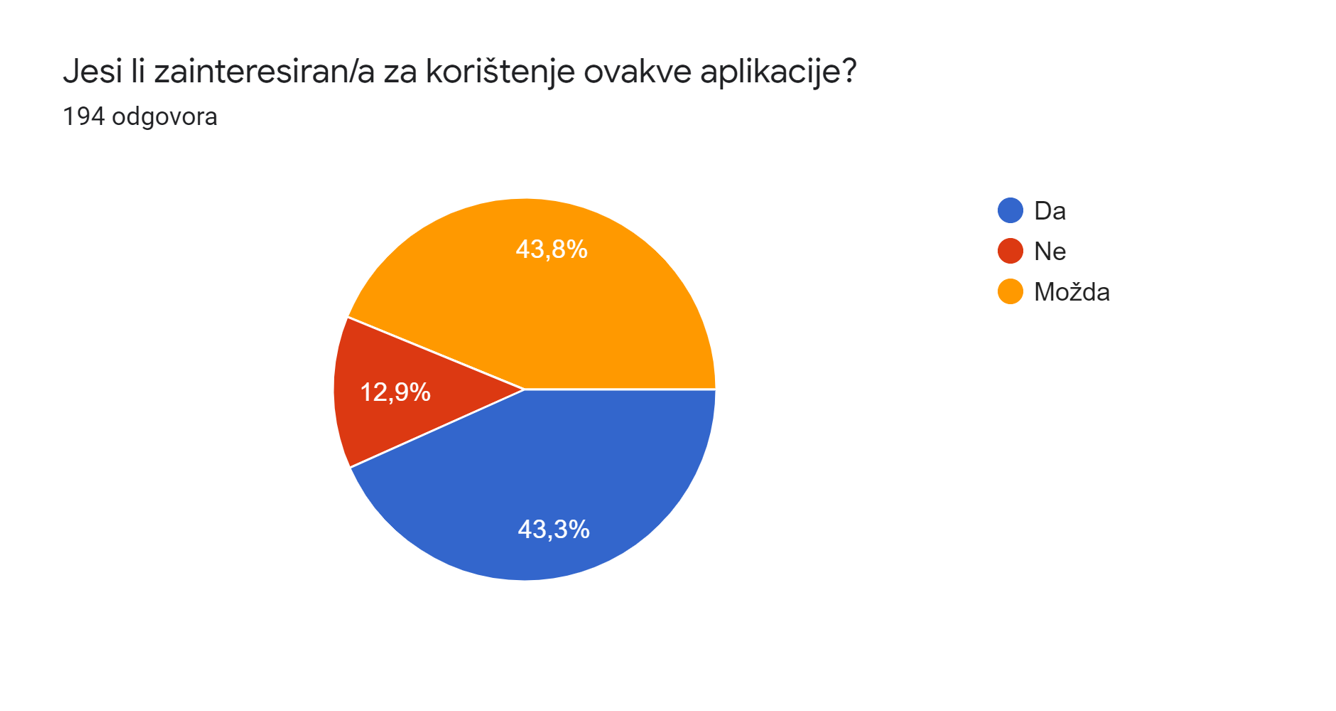
\includegraphics[scale=0.515]{slike/anketa-interes.PNG} 
		    \centering
		    \caption{Rezultat anketnog pitanja o interesu za aplikaciju}
		    \label{fig:anketa-interes}
	    \end{figure}
        
        \noindent Osim pitanja o interesu, naša je anketa služila i odabiru imena aplikacije. Vjerujemo da iza svake dobre aplikacije stoji pamtljivo ime koje ju dobro predstavlja. Uzevši prijedloge svih članova tima složili smo anketno pitanje o odabiru najboljeg i uključili ga u javnu anketu. Rezultat tog dijela ankete jasan je po naslovu dokumenta, a ostale prijedloge i detalje o rezultatu moguće je vidjeti na slici \ref{fig:anketa-ime}.
        
        
        \begin{figure}[H]
		    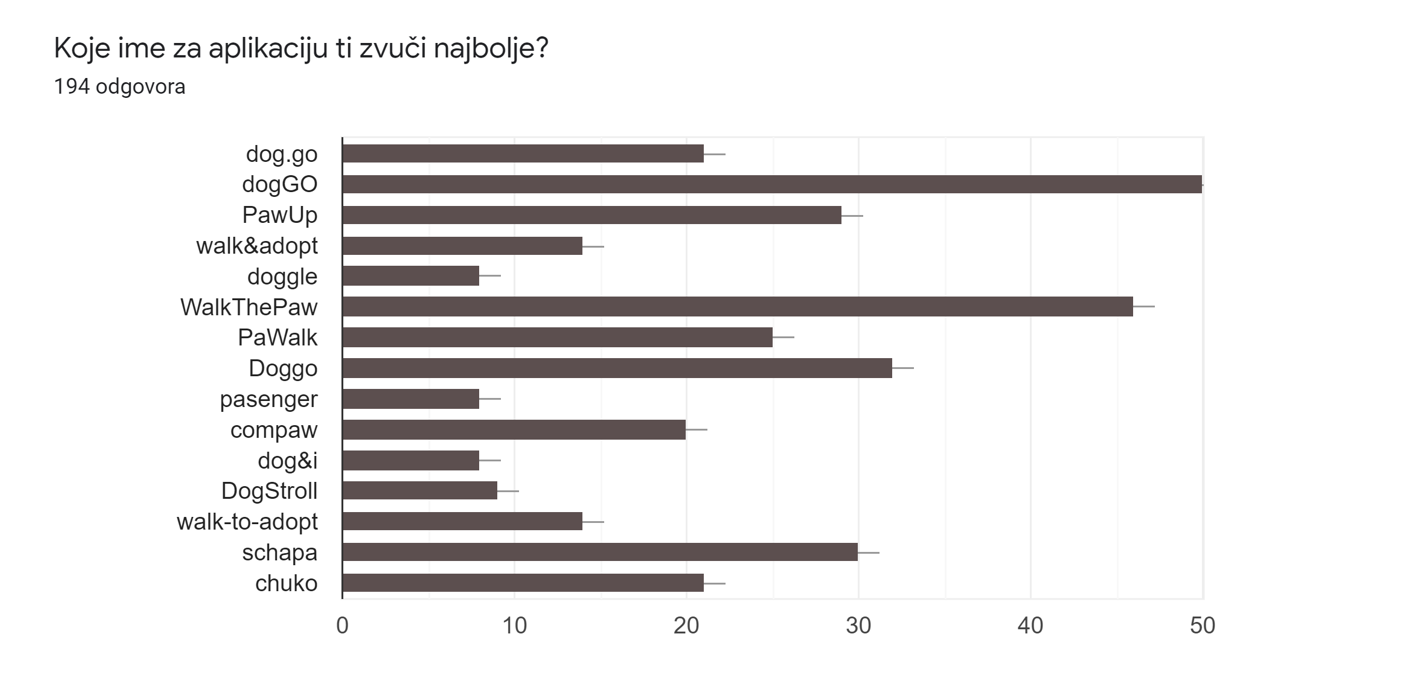
\includegraphics[scale=0.55]{slike/anketa-ime.PNG} 
		    \centering
		    \caption{Rezultat anketnog pitanja o imenu aplikacije}
		    \label{fig:anketa-ime}
	    \end{figure}
    
	\chapter{Specifikacija programske potpore}
		
	\section{Funkcionalni zahtjevi}
		
			
			\noindent \textbf{Dionici:}
			
			\begin{packed_enum}
				
				\item Udruge za životinje
				\item Građani
				\begin{packed_enum}
				    \item registrirani korisnici
				    \item javni posjetitelji
				\end{packed_enum}
				\item Administrator
				\item Razvojni tim
				
			\end{packed_enum}
			
			\noindent \textbf{Aktori i njihovi funkcionalni zahtjevi:}
			
			
			\begin{packed_enum}
				\item  \underbar{Neregistrirani/neprijavljeni korisnik (inicijator) može:}
				
				\begin{packed_enum}
					
					\item pregledati listu svih registriranih udruga
					
					\item pregledati svaku pojedinu registriranu udrugu i dobiti prikaz općih informacija (ime udruge, slika, OIB, e-mail, adresa)
					
					\item pregledati pse pojedine udruge i dobiti prikaz općih  informacija (ime, slika, opis, vrsta šetnje, pasmina, lokacija, raspoloživost)
					
					\item pogledati rang listu registriranih šetača s javnim profilom prema različitim kriterijima:
					\begin{packed_enum}
					    \item broj odrađenih šetnji
					    \item broj različitih šetanih pasa
					    \item duljina odrađenih šetnji
					\end{packed_enum}
			
					\item registrirati se u sustav kao šetač - stvoriti novi korisnički račun za koji su potrebni ime, prezime, korisničko ime, lozinka i e-mail adresa
					
					\item registrirati se u sustav kao udruga - stvoriti novi korisnički račun za koji su potrebni ime, prezime, ime udruge, OIB udruge, lozinka, e-mail
					
					\item prijaviti se već izrađenim korisničkim računom šetača ili udruge u sustav
					
				\end{packed_enum}
			
				\item  \underbar{Udruga (inicijator)  može:}
				
				\begin{packed_enum}
					
					\item kreirati i uređivati profile pasa za koji su potrebni ime, slika, opis, vrsta šetnje (individualna ili skupna), lokacija i raspoloživost  
					
					\item pregledati prošle i nadolazeće rezervacije šetnji za vlastite pse te urediti njihov status  
					
					\item uređivati i izbrisati vlastiti korisnički račun
					
				\end{packed_enum}
				
				\item  \underbar{Šetač (inicijator)  može:}
				
				\begin{packed_enum}
				    \item napraviti, pregledati i urediti status rezervacije psa za šetnju
				    
				    \item pogledati i preuzeti raspored vlastitih šetnji
				    
				    \item pogledati vlastitu statistiku obavljenih šetnji
				    
				    \item omogućiti da vlastita statistika bude javna
				    
				    \item uređivati i izbrisati vlastiti korisnički račun
				    
				\end{packed_enum}
				
				\item  \underbar{Administrator (inicijator)  može:}
				\begin{packed_enum}
				    \item pregledati sve rezervacije te urediti njihov status
				    
				    \item pregledati, uređivati i obrisati sve profile šetača, udruga i pasa
				\end{packed_enum}
				
				\item  \underbar{Baza podataka (sudionik)  može:}
				\begin{packed_enum}
				    \item pohranjuje sve podatke o registriranim šetačima i udrugama
				    
				    \item pohranjuje sve podatke o psima i njihovoj raspoloživosti
				    
				    \item pohranjuje sve podatke o ugovorenim rezervacijama
				\end{packed_enum}
				
			\end{packed_enum}
			
			\eject 
			
			
				
			\subsection{Obrasci uporabe}
				

					\noindent \underbar{\textbf{UC1 - Registracija}}
					\begin{packed_item}
	
						\item \textbf{Glavni sudionik: }Neregistrirani korisnik
						\item  \textbf{Cilj:} Stvoriti korisnički račun šetača ili udruge
						\item  \textbf{Sudionici:} Baza podataka
						\item  \textbf{Preduvjet:} Pristup aplikaciji
						\item  \textbf{Opis osnovnog tijeka:}
						
						\item[] \begin{packed_enum}
	
							\item Korisnik odabire opciju za registraciju šetača ili udruge
							\item Korisnik unosi potrebne korisničke podatke
							\item Korisnik prima obavijest o uspješnoj registraciji
	
						\end{packed_enum}
						
						\item  \textbf{Opis mogućih odstupanja:}
						
						\item[] \begin{packed_item}
	
							\item[2.a] Korisnik je unio neispravni e-mail, podatke u nedozvoljenom formatu ili odabrao već zauzeto korisničko ime i/ili e-mail
							\item[] \begin{packed_enum}
								\item Sustav obavještava korisnika o neuspjelom upisu i vraća ga na stranicu za registraciju
								\item Korisnik mijenja potrebne podatke te završava unos ili odustaje od registracije
							\end{packed_enum}
							
						\end{packed_item}
					\end{packed_item}
					
					
					
					
					
					
					
					
					\noindent \underbar{\textbf{UC2 - Prijava}}
					\begin{packed_item}
	
						\item \textbf{Glavni sudionik:} Neprijavljeni korisnik
						\item  \textbf{Cilj:} Dobiti pristup korisničkom sučelju sustava
						\item  \textbf{Sudionici:} Baza podataka
						\item  \textbf{Preduvjet:} Korisnik registriran u sustav, ali ne i prijavljen
						\item  \textbf{Opis osnovnog tijeka:}
						
						\item[] \begin{packed_enum}
	
							\item Korisnik unosi korisničko ime i lozinku
							\item Sustav provjerava ispravnost unesenih podataka
							\item Korisnik dobiva pristup korisničkim funkcijama 
	
						\end{packed_enum}
						
						\item  \textbf{Opis mogućih odstupanja:}
						
						\item[] \begin{packed_item}
	
							\item[2.a] Korisnik unosi neispravno korisničko ime ili lozinku
							\item[] \begin{packed_enum}
								\item Sustav obavještava korisnika o neuspjeloj prijavi i vraća ga na stranicu za prijavu
							\end{packed_enum}
							
						\end{packed_item}
					\end{packed_item}
					
					
					
					
					
					
					
					
					\noindent \underbar{\textbf{UC3 - Pregled osobnih podataka šetača}}
					\begin{packed_item}
	
						\item \textbf{Glavni sudionik:} Šetač
						\item  \textbf{Cilj:} Pregledati osobne podatke
						\item  \textbf{Sudionici:} Baza podataka
						\item  \textbf{Preduvjet:} Korisnik je prijavljen u sustav kao šetač
						\item  \textbf{Opis osnovnog tijeka:}
						
						\item[] \begin{packed_enum}
							\item Šetač odabire odgovarajuću opciju ”Moj profil”
							\item Aplikacija prikazuje osobne podatke korisnika
						\end{packed_enum}
						
					\end{packed_item}
					
					
					
					
					
					
					
					\noindent \underbar{\textbf{UC4 - Pregled podataka vlastite udruge}}
					\begin{packed_item}
	
						\item \textbf{Glavni sudionik:} Udruga
						\item  \textbf{Cilj:} Pregledati podatke o vlastitoj udruzi
						\item  \textbf{Sudionici:} Baza podataka
						\item  \textbf{Preduvjet:} Korisnik je prijavljen u sustav kao udruga
						\item  \textbf{Opis osnovnog tijeka:}
						
						\item[] \begin{packed_enum}
							\item Udruga odabire opciju ”Moja udruga”
							\item Aplikacija prikazuje podatke o udruzi i psima udruge
						\end{packed_enum}
						
					\end{packed_item}
					
					
					
					
					
					
					
					\noindent \underbar{\textbf{UC5 - Promjena osobnih podataka}}
					\begin{packed_item}
	
						\item \textbf{Glavni sudionik:} Šetač
						\item  \textbf{Cilj:} Promijeniti osobne podatke
						\item  \textbf{Sudionici:} Baza podataka
						\item  \textbf{Preduvjet:} Korisnik je prijavljen u sustav kao šetač
						\item  \textbf{Opis osnovnog tijeka:}
						
						\item[] \begin{packed_enum}
	
							\item Šetač pri pregledu osobnih podataka odabire opciju za promjenu osobnih podataka
							\item Šetač unosi nove podatke
							\item Šetač sprema promjene
							\item Baza podataka se ažurira
	
						\end{packed_enum}
						
						\item  \textbf{Opis mogućih odstupanja:}
						
						\item[] \begin{packed_item}
							\item[3.a] Šetač promijeni podatke, ali novi podatci imaju nedozvoljene vrijednosti
							\item[] \begin{packed_enum}
								\item Sustav obavještava šetača da su unesene nedozvoljene vrijednosti
							\end{packed_enum}
						\end{packed_item}
					\end{packed_item}
				
				
				\noindent \underbar{\textbf{UC6 - Promjena podataka udruge}}
					\begin{packed_item}
	
						\item \textbf{Glavni sudionik:} Udruga
						\item  \textbf{Cilj:} Promijeniti podatke o udruzi
						\item  \textbf{Sudionici:} Baza podataka
						\item  \textbf{Preduvjet:} Korisnik je prijavljen u sustav kao udruga
						\item  \textbf{Opis osnovnog tijeka:}
						
						\item[] \begin{packed_enum}
	
							\item Udruga pri pregledu osobnih podataka odabire opciju za promjenu podataka udruge
							\item Udruga unosi nove podatke
							\item Udruga sprema promjene
							\item Baza podataka se ažurira
	
						\end{packed_enum}
						
						\item  \textbf{Opis mogućih odstupanja:}
						
						\item[] \begin{packed_item}
							\item[3.a] Udruga promijeni podatke, ali novi podatci imaju nedozvoljene vrijednosti
							\item[] \begin{packed_enum}
								\item Sustav obavještava udrugu da su unesene nedozvoljene vrijednosti
							\end{packed_enum}
						\end{packed_item}
					\end{packed_item}
				
				
				
				\noindent \underbar{\textbf{UC7 - Brisanje korisničkog računa}}
					\begin{packed_item}
	
						\item \textbf{Glavni sudionik:} Šetač
						\item  \textbf{Cilj:} Izbrisati korisnički račun
						\item  \textbf{Sudionici:} Baza podataka
						\item  \textbf{Preduvjet:} Korisnik je prijavljen u sustav
						\item  \textbf{Opis osnovnog tijeka:}
						
						\item[] \begin{packed_enum}
	
							\item Šetač odabire opciju ”Moj profil”
							\item Šetač odabire opciju za brisanje računa
							\item Šetač šalje upit je li korisnik siguran
							\item Šetač potvrđuje da je siguran
							\item Otvara se stranica za registraciju
	
						\end{packed_enum}
						
						\item  \textbf{Opis mogućih odstupanja:}
						
						\item[] \begin{packed_item}
							\item[4.a] Šetač odabire da nije siguran
							\item[] \begin{packed_enum}
								\item Sustav vraća šetača na stranicu s osobnim podacima
							\end{packed_enum}
	
						\end{packed_item}
					\end{packed_item}
					
					
					\noindent \underbar{\textbf{UC8 - Brisanje računa udruge}}
					\begin{packed_item}
	
						\item \textbf{Glavni sudionik:} Udruga
						\item  \textbf{Cilj:} Izbrisati račun udruge
						\item  \textbf{Sudionici:} Baza podataka
						\item  \textbf{Preduvjet:} Korisnik je prijavljen u sustav
						\item  \textbf{Opis osnovnog tijeka:}
						
						\item[] \begin{packed_enum}
	
							\item Udruga odabire opciju "Moja udruga"
							\item Udruga odabire opciju za brisanje računa
							\item Udruga šalje upit je li korisnik siguran
							\item Udruga potvrđuje da je siguran
							\item Baza podataka označava da je šetač obrisan
							\item Otvara se stranica za registraciju
	
						\end{packed_enum}
						
						\item  \textbf{Opis mogućih odstupanja:}
						
						\item[] \begin{packed_item}
							\item[4.a] Udruga odabire da nije sigurna
							\item[] \begin{packed_enum}
								\item Sustav vraća korisnika na stranicu s podacima udruge
							\end{packed_enum}
	
						\end{packed_item}
					\end{packed_item}
					
					
					
					\noindent \underbar{\textbf{UC9 - Pregled udruga}}
					\begin{packed_item}
	
						\item \textbf{Glavni sudionik:} Neregistrirani korisnik, šetač, udruga
						\item  \textbf{Cilj:} Pregledati registrirane udruge i dobiti prikaz općih informacija
						\item  \textbf{Sudionici:} Baza podataka
						\item  \textbf{Preduvjet:} Pristup aplikaciji
						\item  \textbf{Opis osnovnog tijeka:}
						
						\item[] \begin{packed_enum}
							\item Korisnik odabire opciju “Pregledaj udruge”
							\item Aplikacija prikazuje sve udruge upisane u bazu podataka i osnovne informacije
						\end{packed_enum}
						
					\end{packed_item}
					
					
					
					
					
					\noindent \underbar{\textbf{UC10 - Pregled detalja udruge}}
					\begin{packed_item}
	
						\item \textbf{Glavni sudionik:} Neregistrirani korisnik, šetač, udruga
						\item  \textbf{Cilj:} Pregled detaljnijih informacija o odabranoj udruzi
						\item  \textbf{Sudionici:} Baza podataka
						\item  \textbf{Preduvjet:} Pristup aplikaciji
						\item  \textbf{Opis osnovnog tijeka:}
						
						\item[] \begin{packed_enum}
							\item Korisnik na listi svih udruga odabire udrugu koju želi pregledati
							\item Aplikacija prikazuje detaljne podatke o odabranoj udruzi i sve njene pse
						\end{packed_enum}
						
					\end{packed_item}
					
					
					
					
					
					\noindent \underbar{\textbf{UC11 - Pregled detalja psa}}
					\begin{packed_item}
	
						\item \textbf{Glavni sudionik:} Neregistrirani korisnik, šetač, udruga
						\item  \textbf{Cilj:} Pregled detaljnijih informacija o odabranom psu
						\item  \textbf{Sudionici:} Baza podataka
						\item  \textbf{Preduvjet:} Pristup aplikaciji
						\item  \textbf{Opis osnovnog tijeka:}
						
						\item[] \begin{packed_enum}
							\item Korisnik se nalazi na profilu udruge
							\item Aplikacija prikazuje detaljne podatke o odabranom psu i nudi opciju rezervacije
						\end{packed_enum}
						
					\end{packed_item}
					
					\noindent \underbar{\textbf{UC12 - Rezervacija šetnje}}
					\begin{packed_item}
	
						\item \textbf{Glavni sudionik:} Šetač
						\item  \textbf{Cilj:} Rezervirati termin šetnje odabranog psa
						\item  \textbf{Sudionici:} Baza podataka
						\item  \textbf{Preduvjet:} Pristup aplikaciji
						\item  \textbf{Opis osnovnog tijeka:}
						
						\item[] \begin{packed_enum}
							\item Šetač odabire opciju rezervacije za odabranog psa
							\item Aplikacija prikazuje raspoloživost psa, nudi opciju rezervacije termina i opciju grupne šetnje
							\item Šetač odabire slobodan termin za individualnu šetnju psa
							\item Šetač potvrđuje svoj odabir
							\item Šetač dobiva potvrdu o rezervaciji
						\end{packed_enum}
						
						\item  \textbf{Opis mogućih odstupanja:}
						
						\item[] \begin{packed_item}
							\item[2.a] Korisnik još nije registriran u sustav
							\item[] \begin{packed_enum}
								\item Sustav vodi korisnika na stranicu registracije
							\end{packed_enum}
							\item[3.a] Šetač odabire opciju grupne šetnje
							\item[] \begin{packed_enum}
								\item Aplikacija prikazuje ostale dostupne pse iz iste udruge u odabranom terminu
								\item Šetač odabire željene pse za dodati u rezervaciju šetnje
								\item Šetač potvrđuje svoj odabir
								\item Šetač dobiva potvrdu o rezervaciji
							\end{packed_enum}
	
						\end{packed_item}
					\end{packed_item}
					
					
					
					
					\noindent \underbar{\textbf{UC13 - Pregled kalendara}}
					\begin{packed_item}
	
						\item \textbf{Glavni sudionik:} Šetač
						\item  \textbf{Cilj:} Pregledati vlastiti raspored ugovorenih šetnji
						\item  \textbf{Sudionici:} Baza podataka
						\item  \textbf{Preduvjet:} Korisnik je prijavljen kao šetač
						\item  \textbf{Opis osnovnog tijeka:}
						
						\item[] \begin{packed_enum}
							\item Šetač se nalazi na kartici Moj profil
							\item Aplikacija prikazuje sve ugovorene šetnje korisnika i opciju preuzimanja rasporeda u pdf formatu
						\end{packed_enum}
					\end{packed_item}
					
					
					\noindent \underbar{\textbf{UC14 - Preuzimanje rasporeda}}
					\begin{packed_item}
	
						\item \textbf{Glavni sudionik:} Šetač
						\item  \textbf{Cilj:} Preuzeti vlastiti raspored ugovorenih šetnji
						\item  \textbf{Sudionici:} Baza podataka
						\item  \textbf{Preduvjet:} Korisnik je prijavljen kao šetač
						\item  \textbf{Opis osnovnog tijeka:}
						
						\item[] \begin{packed_enum}
							\item Šetač pri pregledu vlastitog kalendara odabire opciju preuzimanja rasporeda u pdf formatu
							\item Aplikacija prikazuje opcije vremenskog razdoblja sadržanog u pdf rasporedu
							\item Šetač odabire željenu opciju
							\item Na šetačevo računalo preuzima se raspored odabranog vremenskog razdoblja
							
						\end{packed_enum}
					\end{packed_item}
					
					
					
					
					
						\noindent \underbar{\textbf{UC15 - Brisanje rezervacije od strane šetača}}
					\begin{packed_item}
	
						\item \textbf{Glavni sudionik:} Šetač
						\item  \textbf{Cilj:} Obrisati prethodno ugovorenu šetnju
						\item  \textbf{Sudionici:} Baza podataka
						\item  \textbf{Preduvjet:} Korisnik ima ugovorenu barem jednu rezervaciju 
						\item  \textbf{Opis osnovnog tijeka:}
						
						\item[] \begin{packed_enum}
							\item Šetač pri pregledu ugovorenih šetnji odabire odgovarajuću rezervaciju i odabire opciju brisanja
							\item Sustav šalje upit je li korisnik siguran
							\item Šetač potvrđuje da je siguran
							\item Aplikacija ponovno prikazuje stranicu sa svim ugovorenim šetnjama
						
						\end{packed_enum}
						\item  \textbf{Opis mogućih odstupanja:}
						
						\item[] \begin{packed_item}
							\item[3.a] Korisnik odabire da nije siguran
							\item[] \begin{packed_enum}
								\item Sustav vraća korisnika na stranicu "Moj profil"
							\end{packed_enum}
	                        \item[4.a] Brisanje nije uspješno obavljeno
	                        \item[] \begin{packed_enum}
								\item Aplikacija prikazuje povratnu informaciju o greški prilikom brisanja
							\end{packed_enum}
						\end{packed_item}
					\end{packed_item}
					
					
					
					
					
					\noindent \underbar{\textbf{UC16 - Pregled svih rezerviranih šetnji udruge}}
					\begin{packed_item}
	
						\item \textbf{Glavni sudionik:} Udruga
						\item  \textbf{Cilj:} Pregledati sve rezervacije pasa vlastite udruge
						\item  \textbf{Sudionici:} Baza podataka
						\item  \textbf{Preduvjet:} Korisnik je prijavljen kao udruga
						\item  \textbf{Opis osnovnog tijeka:}
						
						\item[] \begin{packed_enum}
							\item Udruga odabire opciju pregleda rezervacija
							\item Aplikacija prikazuje sve buduće i prošle ugovorene šetnje za pse vlastite udruge
						\end{packed_enum}
					\end{packed_item}
					
					\noindent \underbar{\textbf{UC17 - Brisanje rezervacije od strane udruge}}
					\begin{packed_item}
	
						\item \textbf{Glavni sudionik:} Udruga
						\item  \textbf{Cilj:} Obrisati prethodno ugovorenu šetnju
						\item  \textbf{Sudionici:} Baza podataka
						\item  \textbf{Preduvjet:} Pas udruge ima ugovorenu barem jednu rezervaciju 
						\item  \textbf{Opis osnovnog tijeka:}
						
						\item[] \begin{packed_enum}
							\item Udruga pri pregledu svih ugovorenih šetnji odabire odgovarajuću rezervaciju i odabire opciju brisanja
							\item Sustav šalje upit je li udruga sigurna
							\item Udruga potvrđuje da je sigurna
							\item Aplikacija ponovno prikazuje stranicu sa svim ugovorenim šetnjama
						
						\end{packed_enum}
						\item  \textbf{Opis mogućih odstupanja:}
						
						\item[] \begin{packed_item}
							\item[3.a] Udruga odabire da nije sigurna
							\item[] \begin{packed_enum}
								\item Sustav vraća korisnika na stranicu "Moj profil"
							\end{packed_enum}
	                        \item[4.a] Brisanje nije uspješno obavljeno
	                        \item[] \begin{packed_enum}
								\item Aplikacija prikazuje povratnu informaciju o greški prilikom brisanja
							\end{packed_enum}
						\end{packed_item}
					\end{packed_item}
					
					
					
					\noindent \underbar{\textbf{UC18 - Pregled pasa vlastite udruge}}
					\begin{packed_item}
	
						\item \textbf{Glavni sudionik:} Udruga
						\item  \textbf{Cilj:} Pregledati sve informacije o određenom psu iz vlastite udruge
						\item  \textbf{Sudionici:} Baza podataka
						\item  \textbf{Preduvjet:} Korisnik je prijavljen kao udruga
						\item  \textbf{Opis osnovnog tijeka:}
						
						\item[] \begin{packed_enum}
							\item Udruga pri pregledu podataka o udruzi odabire opciju pregleda željenog psa
							\item Aplikacija prikazuje sve informacije o psu i odgovarajuće šetnje
							
						\end{packed_enum}
					\end{packed_item}
					
					
					
					
					\noindent \underbar{\textbf{UC19 - Dodavanje psa u udrugu}}
					\begin{packed_item}
	
						\item \textbf{Glavni sudionik:} Udruga
						\item  \textbf{Cilj:} Dodati novog psa u aplikaciju
						\item  \textbf{Sudionici:} Baza podataka
						\item  \textbf{Preduvjet:} Korisnik je prijavljen kao udruga
						\item  \textbf{Opis osnovnog tijeka:}
						
						\item[] \begin{packed_enum}
							\item Udruga pri pregledu podataka o udruzi odabire opciju za dodavanje psa
							\item Aplikacija otvara formu za upis informacija o psu
							\item Udruga sprema upisane podatke
							\item Novi podaci pohranjuju se u bazu podataka
							\item Udruga dobiva potvrdu o uspješnom izvršenju
							\item Aplikacija prikazuje sve informacije o psu i odgovarajuće šetnje
							
						\end{packed_enum}
						
						\item  \textbf{Opis mogućih odstupanja:}
						
						\item[] \begin{packed_item}
							\item[3.a] Udruga unese podatke o psu, ali ne spremi upis
							\item[] \begin{packed_enum}
								\item Sustav obavještava korisnika da nije spremio podatke prije izlaska iz prozora
							\end{packed_enum}
						\end{packed_item}
					\end{packed_item}
					
					
					
					
					\noindent \underbar{\textbf{UC20 - Brisanje psa}}
					\begin{packed_item}
	
						\item \textbf{Glavni sudionik:} Udruga
						\item  \textbf{Cilj:} Obrisati psa iz sustava
						\item  \textbf{Sudionici:} Baza podataka
						\item  \textbf{Preduvjet:} Korisnik je prijavljen kao udruga
						\item  \textbf{Opis osnovnog tijeka:}
						
						\item[] \begin{packed_enum}
							\item Udruga pri pregledu svih pasa odabire opciju pregleda željenog psa
							\item Udruga odabire opciju brisanja psa iz aplikacije
							\item Sustav šalje upit korisniku je li siguran
							\item Udruga potvrđuje da je siguran
							\item Sustav šalje korisnika natrag na stranicu sa psima
							
						\end{packed_enum}
						
						\item  \textbf{Opis mogućih odstupanja:}
						
						\item[] \begin{packed_item}
							\item[4.a] Udruga odabire da nije siguran
							\item[] \begin{packed_enum}
								\item Sustav vraća korisnika na stranicu sa psima
							\end{packed_enum}
	
						\end{packed_item}
					\end{packed_item}
					
					
					\noindent \underbar{\textbf{UC21 - Pregled rang liste}}
					\begin{packed_item}
	
						\item \textbf{Glavni sudionik:} Neregistrirani korisnik, šetač, udruga
						\item  \textbf{Cilj:} Pregledati rang listu svih javnih šetača
						\item  \textbf{Sudionici:} Baza podataka
						\item  \textbf{Preduvjet:} Pristup aplikaciji
						\item  \textbf{Opis osnovnog tijeka:}
						
						\item[] \begin{packed_enum}
							\item Korisnik odabire opciju "Šetači"
							\item Aplikacija prikazuje rang listu svih šetača prema zadanom kriteriju
						\end{packed_enum}
					\end{packed_item}
					
					\noindent \underbar{\textbf{UC22 - Pregled svih šetača i udruga}}
					\begin{packed_item}
	
						\item \textbf{Glavni sudionik:} Administrator
						\item  \textbf{Cilj:} Pregledati sve šetače i udruge u sustavu
						\item  \textbf{Sudionici:} Baza podataka
						\item  \textbf{Preduvjet:} Korisnik je prijavljen kao administrator
						\item  \textbf{Opis osnovnog tijeka:}
						
						\item[] \begin{packed_enum}
							\item Administrator odabire opciju za pregled svih korisnika sustava
							\item Aplikacija prikazuje listu svih šetača i svih udruga
						\end{packed_enum}
					\end{packed_item}
					
					\noindent \underbar{\textbf{UC23 - Pregled svih rezervacija svih udruga}}
					\begin{packed_item}
	
						\item \textbf{Glavni sudionik:} Administrator
						\item  \textbf{Cilj:} Pregledati sve rezervacije svih udruga
						\item  \textbf{Sudionici:} Baza podataka
						\item  \textbf{Preduvjet:} Korisnik je prijavljen kao administrator
						\item  \textbf{Opis osnovnog tijeka:}
						
						\item[] \begin{packed_enum}
							\item Administrator odabire opciju za pregled svih rezervacija
							\item Aplikacija prikazuje listu svih rezervacija po udrugama
						\end{packed_enum}
					\end{packed_item}
					
					\noindent \underbar{\textbf{UC24 - Promjena statusa rezervacije}}
					\begin{packed_item}
	
						\item \textbf{Glavni sudionik:} Administrator
						\item  \textbf{Cilj:} Promijeniti status rezervacije (aktivna, otkazana)
						\item  \textbf{Sudionici:} Baza podataka
						\item  \textbf{Preduvjet:} Korisnik je prijavljen kao administrator
						\item  \textbf{Opis osnovnog tijeka:}
						
						\item[] \begin{packed_enum}
							\item Administrator odabire rezervaciju čiji status želi promijeniti
							\item Administrator mijenja status rezervacije
						\end{packed_enum}
					\end{packed_item}
					
					
				\subsubsection{Dijagrami obrazaca uporabe}
					
					\begin{figure}[H]
		                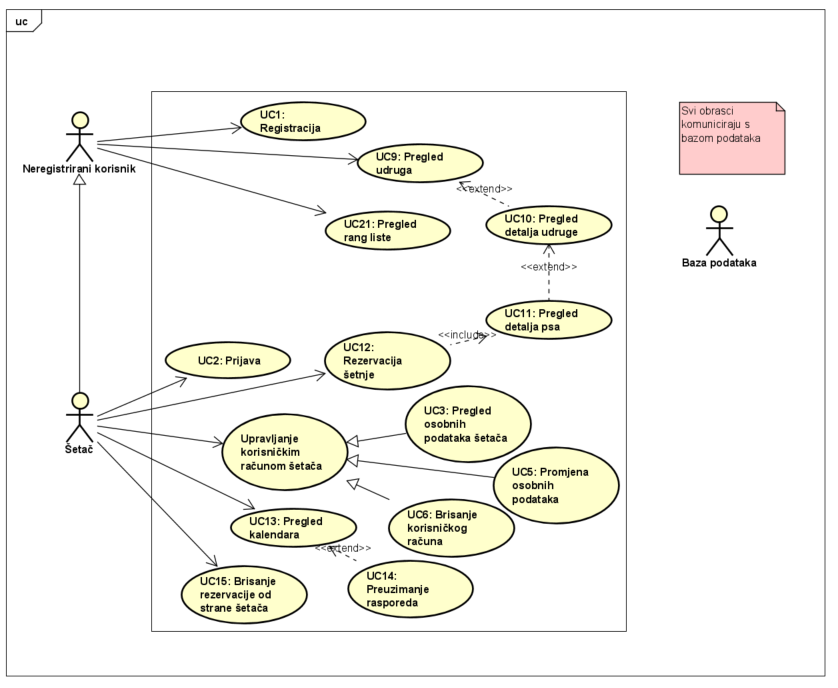
\includegraphics[scale=0.9]{dijagrami/uc-dijagram-1.PNG} 
	                	\centering
	                   	\caption{Dijagram obrasca uporabe, funkcionalnost neregistriranog korisnika i šetača}
	                	\label{fig:uc-1}
	                \end{figure}
	                
	                \begin{figure}[H]
		                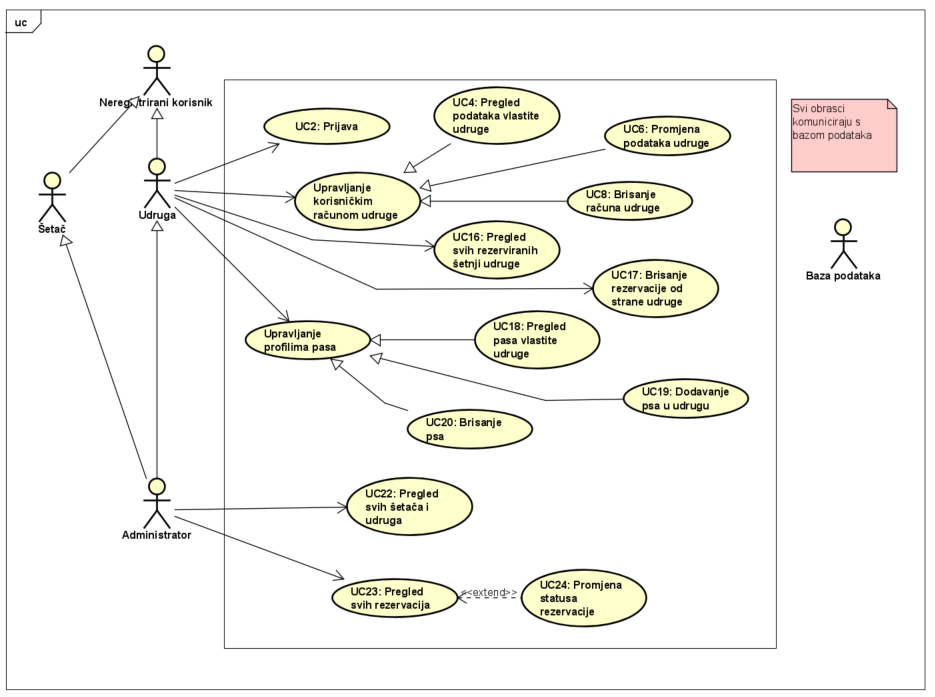
\includegraphics[scale=0.9]{dijagrami/uc-dijagram-2.PNG} 
	                	\centering
	                   	\caption{Dijagram obrasca uporabe, funkcionalnost udruge i administratora}
	                	\label{fig:uc-1}
	                \end{figure}
	                
				\eject		
				
			\subsection{Sekvencijski dijagrami}
				
				\noindent \textbf{Obrazac uporabe UC1 - Registracija}\\
				Korisnik bira opciju za registraciju šetača ili udruge te šalje zahtjev za registraciju. Poslužitelj prikazuje formu za odabranu registraciju. Korisnik unosi potrebne korisničke podatke. Poslužitelj provjerava ispravnost unesenih podataka i ako su valjani, u bazu podataka sprema podatke novog korisnika i obavještava ga o uspješnoj registraciji. Ako su elektronička pošta, korisničko ime ili formati nedozvoljeni, korisnika se obavještava o neuspješnoj registraciji i vraća na stranicu za registraciju.
				
				\begin{figure}[H]
					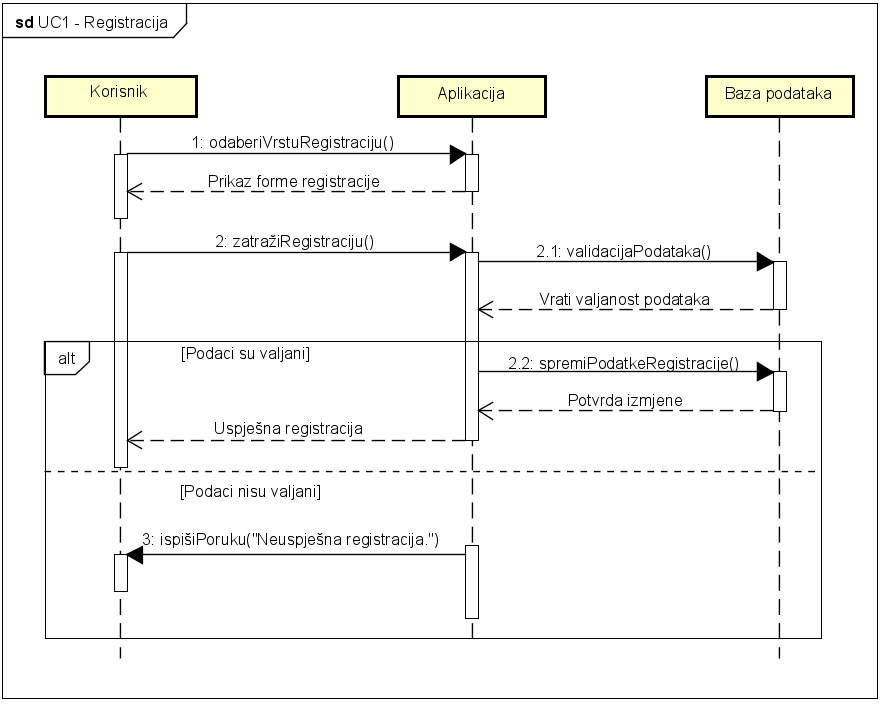
\includegraphics[scale=0.7]{dijagrami/UC1-Registracija.PNG} 
					\centering
					\caption{Sekvencijski dijagram za registraciju korisnika}
					\label{fig:uc-1}
				\end{figure}
				
				\eject
				
				\noindent \textbf{Obrazac uporabe UC5 - Promjena osobnih podataka}\\
				Korisnik bira opciju “Promijeni osobne podatke”. Poslužitelj vraća formu za unos novih podataka. Korisnik potom unosi nove podatke i potvrđuje promjenu. Poslužitelj provjerava valjanost novih podataka preko baze podataka. Ako su podaci valjani, poslužitelj šalje podatke korisnika u bazu podataka kako bi se stare vrijednosti ažurirale. Baza podataka vraća potvrdu poslužitelju koja šalje poruku o uspješnoj promijeni. U suprotnom, korisnika se obavještava o neuspješnoj promjeni podataka.
				
				\begin{figure}[H]
					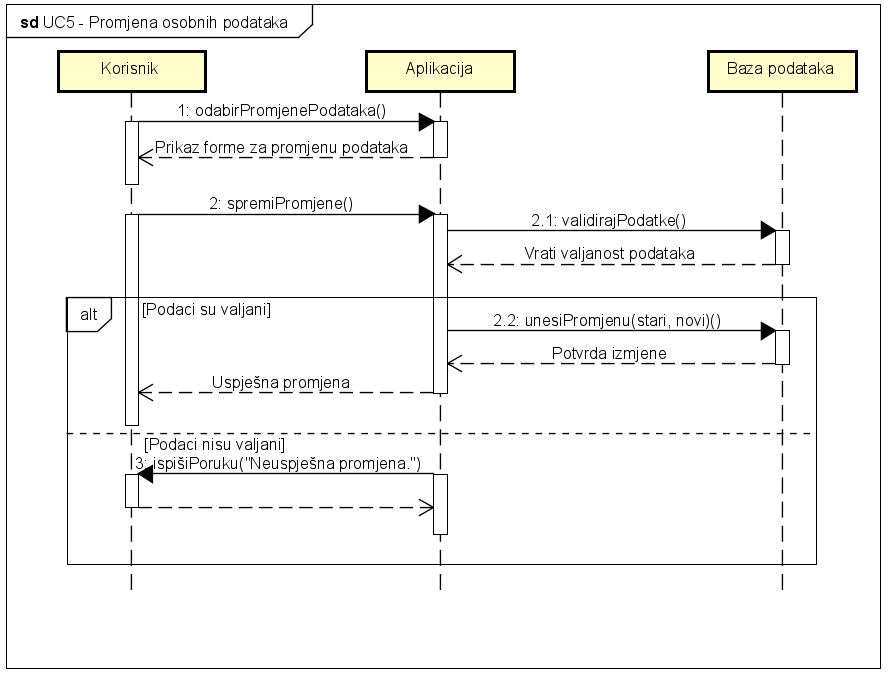
\includegraphics[scale=0.7]{dijagrami/UC5-Promjena-osobnih-podataka.PNG} 
					\centering
					\caption{Sekvencijski dijagram za promjenu osobnih podataka korisnika}
					\label{fig:uc-1}
				\end{figure}
				
				\eject
				
				\noindent \textbf{Obrazac uporabe UC12 - Rezervacija šetnje}\\
				Korisnik bira opciju “Odaberi psa.”. Ako korisnik nije registriran, sustav navodi korisnika na stranicu za registraciju. Poslužitelj korisniku vraća opciju za rezervaciju pasa. Korisnik bira određenog psa na što poslužitelj prikazuje njegovu raspoloživost te nudi opciju rezervacije. Korisnik bira termin na što mu poslužitelj vraća prikaz odabira i opciju grupne šetnje. Korisnik potvrđuje svoj odabir ako se odluči za individualnu šetnju. Odabirom opcije grupne šetnje poslužitelj iz baze dohvaća dostupne pse iz iste udruge u odabranom terminu i prikazuje korisniku. Korisnik bira pse za grupnu šetnju i potvrđuje svoj odabir, nakon čega poslužitelj dodaje novu rezervaciju u bazu koja vraća poruku potvrde i obavještava korisnika o uspješnoj rezervaciji.
				
				\begin{figure}[H]
					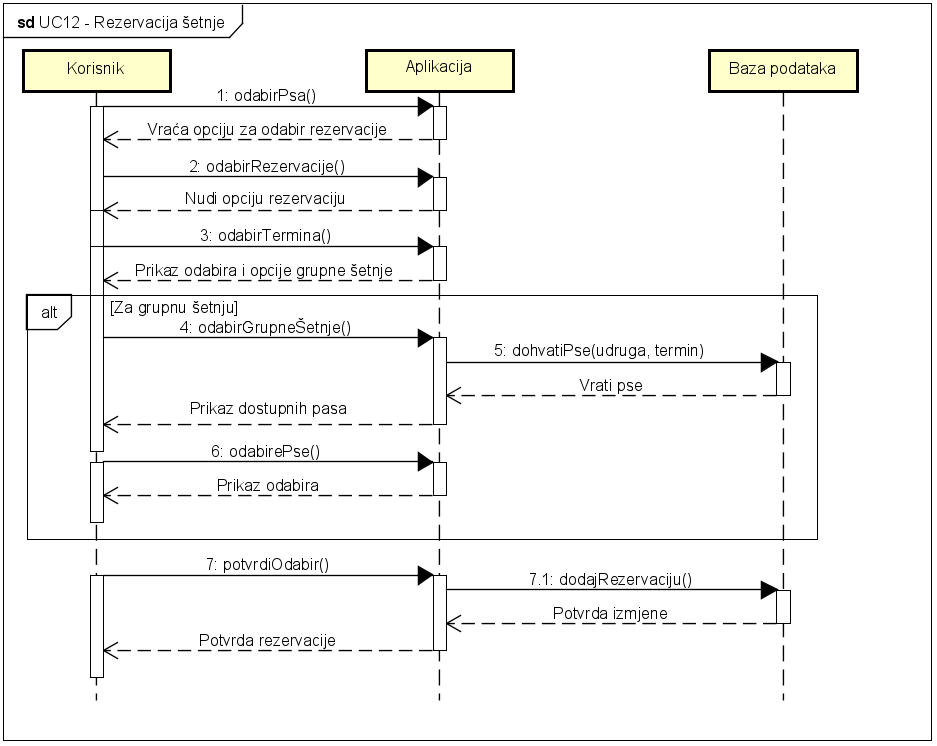
\includegraphics[scale=0.7]{dijagrami/UC12-Rezervacija-setnje.PNG} 
					\centering
					\caption{Sekvencijski dijagram za rezerviranje šetnji}
					\label{fig:uc-1}
				\end{figure}
				
				\eject
				
				
				
		\section{Ostali zahtjevi}
		
		    
		    \begin{packed_item}
		        \item Sustav treba biti implementiran kao web-aplikacija koristeći objektno orijentiranu paradigmu
		        \item Sustav treba omogućiti rad više korisnika u stvarnom vremenu
		        \item Sustav treba podržavati funkcionalnosti neovisno o vrsti uređaja, preglednika ili veličini ekrana
		        \item Nadogradnja sustava ne smije narušavati postojeće funkcionalnosti sustava
		        \item Veza s bazom podataka mora biti kvalitetno zaštićena, brza i otporna na vanjske greške
		        \item Izvršavanje dijela programa u kojem se pristupa bazi podataka ne smije trajati dulje od nekoliko sekundi
		        \item Korisnički podaci trebaju biti sigurno pohranjeni i odgovarajuće enkriptirani
		        \item Pristup sustavu mora biti omogućen iz javne mreže
		        \item Korisničko sučelje treba biti jednostavno, intuitivno i pregledno, korisnici se moraju znati koristiti sučeljem bez opširnih uputa
		        \item Neispravno korištenje korisničkog sučelja ne smije narušiti funkcionalnost i rad sustava
		        \item Korisničko sučelje i sustav moraju podržavati hrvatsku abecedu (dijakritičke znakove) pri unosu i prikazu tekstualnog sadržaja
		        \item Sustav treba koristiti odgovarajući europski format datuma (\textit{DD.MM.YYYY.})
		        
		    \end{packed_item}
		    
	
	\chapter{Arhitektura i dizajn sustava}

		
	\noindent Ključne komponente za ostvarenje našeg sustava: 
	   \begin{packed_item}
	        \item Web poslužitelj 
	        \item Web aplikacija 
	        \item Baza podataka
	    \end{packed_item}
	    
	
	%ARHITEKTURA SUSTAVA
	\begin{figure}[H]
		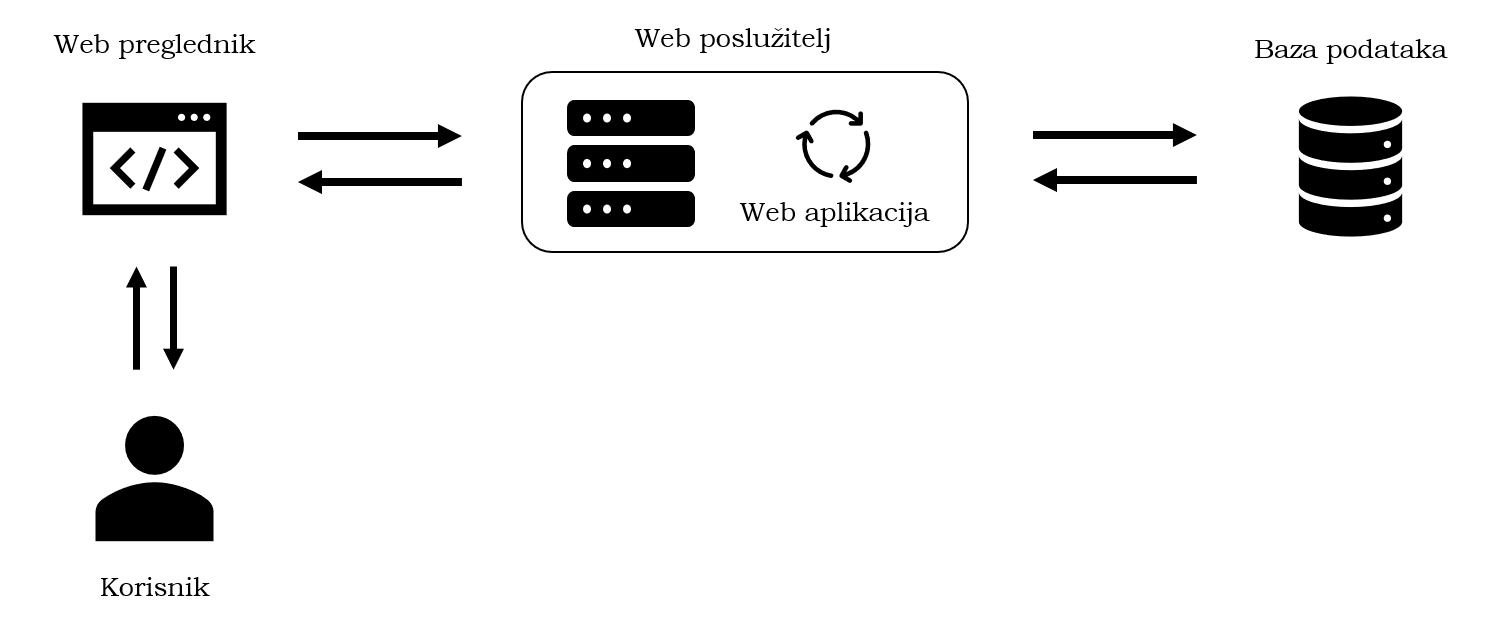
\includegraphics[scale=0.48]{slike/system-architecture.PNG} 
		\centering
		\caption{Arhitektura sustava}
		\label{fig:arhitektura}
	\end{figure}
		
	\noindent Komunikacija krajnjeg korisnika s našim sustavom započinje u web pregledniku pristupom iz javne mreže preko odgovarajuće poveznice. Konceptualnu shemu navedenog sustava moguće je pratiti na slici \ref{fig:arhitektura}.	 \par
	
	\medskip
	
	\noindent \underbar{Web preglednik} (engl. \textit{web browser}) program je koji korisniku omogućuje pronalaženje i pregled podataka na Internetu u obliku web stranica. Pruža grafičko sučelje i prikaz multimedijalnih sadržaja dohvaćenih s poslužitelja te prati korisničke akcije nad sučeljem kako bi generirao odgovarajuće zahtjeve i delegirao posao prema dijelu sustava koji ih obrađuje. Korišteni tip zahtjeva jest HTTP (engl. \textit{Hyper Text Transfer Protocol}). \par
	
	\medskip
	
	\noindent \underbar{Web poslužitelj} (engl. \textit{web server}) prima zahtjeve web preglednika. U našoj implementaciji pristupa mu se pomoću REST (engl. \textit{Representational State Transfer}) usluga koje koriste JSON format. Pokreće komunikaciju s web aplikacijom i prosljeđuje joj korisničke zahtjeve.  \par
	
	\medskip
	
	\noindent \underbar{Web aplikacija} (engl. \textit{web app}) je ključni dio sustava koji obrađuje korisničke zahtjeve. Obrada uključuje određenu komunikaciju s bazom podataka poput dohvata, uređivanja ili brisanja. Nakon što se odgovarajuće procesuira zahtjev, šalje se odgovor poslužitelju koji se ultimativno prikazuje korisniku u web pregledniku. \par
	
	
	
	\bigskip    
	
	
	
	\noindent Naš se produkt konceptualno temelji na troslojnoj arhitekturi kojom se najčešće koriste poslovne aplikacije i sastoji se od sljedećih slojeva:
	 \begin{packed_enum}
	        \item \textbf{Prezentacijski sloj} - korisničko sučelje aplikacije koje korisniku predstavlja značajke i podatke aplikacije
	        \item \textbf{Servisni sloj} - sadrži poslovnu logiku koja pokreće osnovne funkcionalnosti aplikacije poput donošenja odluka, izračuna, procjena i obrade podataka koji prolaze između druga dva sloja
	        \item \textbf{Podatkovni sloj} - odgovoran za interakciju s bazama podataka radi spremanja i vraćanja podataka aplikacije
	    \end{packed_enum}
	
	\bigskip
	
	\noindent Specifičnije, korišteni Spring razvojni okvir koristi se i MVC arhitekturom (eng. \textit{Model-View-Controller}). To podrazumijeva sljedeću podjelu uloga vidljivoj i na slici \ref{fig:mvc}.
	 \begin{packed_item}
	        \item \textbf{Model} - dohvat i manipulacija podatcima
	        \item \textbf{Pogled} - prezentacija dostavljenih podataka
	        \item \textbf{Nadglednik}  - prima zahtjeve te upravlja s pogledom i modelom
	 \end{packed_item}
	 
	%MVC ARHITEKTURA
	\begin{figure}[H]
		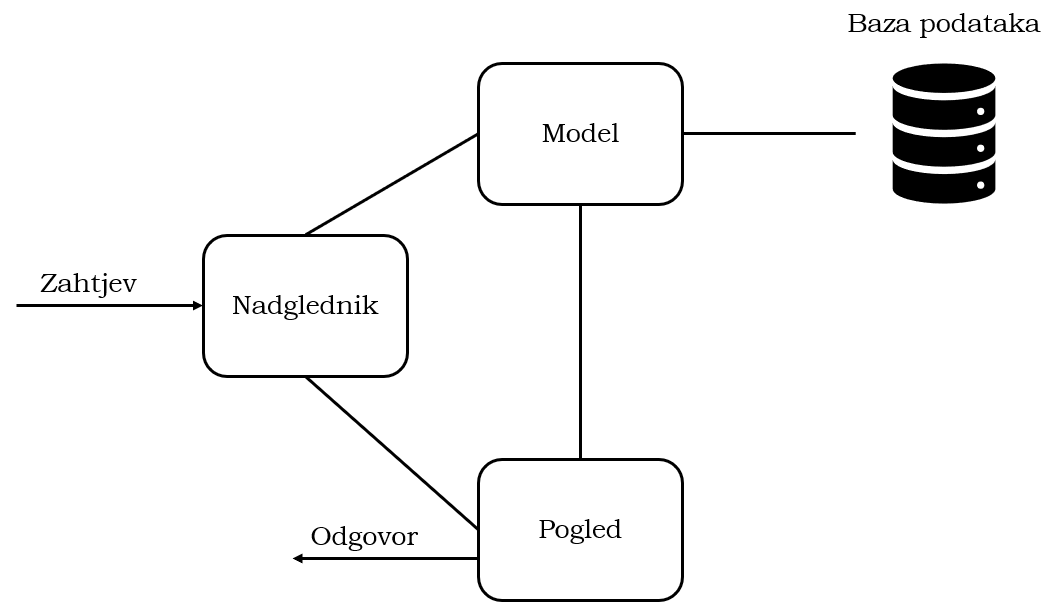
\includegraphics[scale=0.55]{slike/mvc-architecture.PNG} 
		\centering
		\caption{MVC arhitektura}
		\label{fig:mvc}
	\end{figure}
	
	\newpage

	
	 U prošlosti se linearnost troslojnog modela smatrala poželjnom, no razvojem web tehnologija "trokutasti" MVC model dobio je na popularnosti pa danas mnogi sustavi koriste hibridnu formu navedenih arhitekturnih oblika pa tako i Spring razvojni okvir. 
	
	%HIBRIDNA ARHITEKTURA
	\begin{figure}[H]
		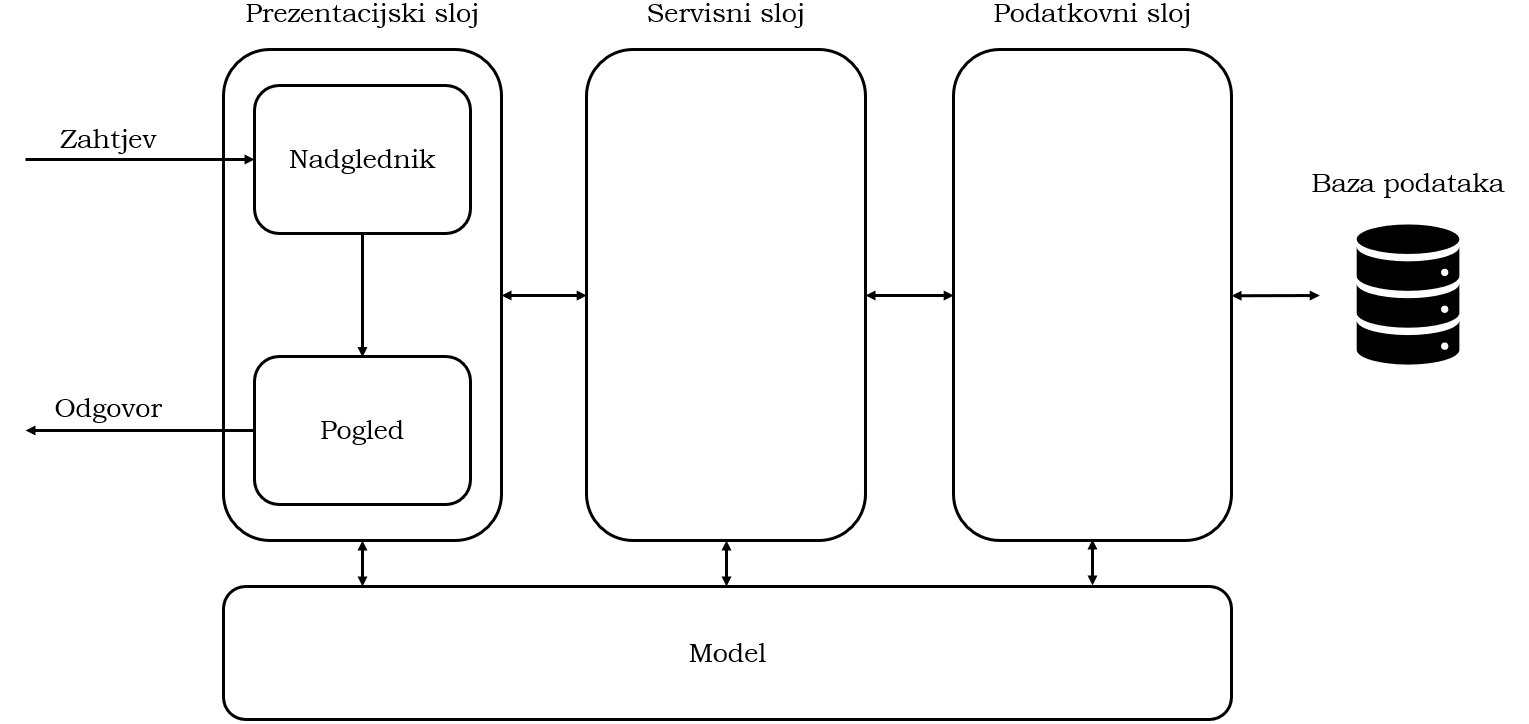
\includegraphics[scale=0.47]{slike/hybrid-architecture.PNG} 
		\centering
		\caption{Konceptualno hibridna arhitektura Spring razvojnog okvira}
		\label{fig:hibridna}
	\end{figure}
		

				
		\section{Baza podataka}
			
		
			Kako bi olakšali modeliranje stvarnog svijeta korištena je relacijska baza podataka. Modelirana je relacijama, odnosno tablicama koje imaju svoje ime i atribute. Tablice su različito povezane preko zajedničkih atributa. Baza podataka služi za brzu i jednostavnu pohranu podataka, izmjenu, ažuriranje te dohvat podataka za daljnju obradu. Ova aplikacija koristi bazu podataka sa sljedećim entitetima:
			
			\begin{packed_item}
				
				\item  RegisteredUser
				\item  RegisteredUserLogin
				\item  Association
				\item  AssociationLogin
				\item  Dog
				\item  WalkJournal
				\item  AssociationLocation
				\item  DogAvailability
				\item  RankingList
				\item  OtherReservations
				
			\end{packed_item} 
		
			\subsection{Opis tablica}
			
					\noindent \textbf{Walker} Entitet sadrži sve bitne informacije o registriranom korisniku aplikacije. Njegovi atributi su: ID korisnika, ime i prezime, elektronička pošta i broj mobitela korisnika, javnost podataka i obrisan (atribut koji postaje true ako korisnik obriše svoj račun). Entitet RegisteredUser je u \textit{Many-to-One} vezi s entitetom RankingList preko jedinstvenog identifikatora korisnika i u \textit{One-to-Many} vezi s entitetom WalkJournal preko jedinstvenog identifikatora korisnika.
				
				\begin{longtabu} to \textwidth {|X[8, l]|X[6, l]|X[18, l]|}
					
					\hline \multicolumn{3}{|c|}{\textbf{Walker}}	 \\[3pt] \hline
					\endfirsthead
					
					\hline \multicolumn{3}{|c|}{\textbf{Walker}}	 \\[3pt] \hline
					\endhead
					
					\hline 
					\endlastfoot
					
					\cellcolor{LightGreen}UserID & BIGINT	&  	Jedinstveni identifikator korisnika 	\\ \hline 
					FirstName & VARCHAR	& Ime korisnika 		\\ \hline
					LastName & VARCHAR & Prezime korisnika \\ \hline
					Email & VARCHAR & Elektronička pošta korisnika \\ \hline
					PhoneNumber & VARCHAR & Broj mobitela korisnika \\ \hline
					Public & BOOLEAN & Javnost podataka korisnika \\ \hline
					Deleted & BOOLEAN & Račun obrisan \\ \hline
					
					
				\end{longtabu}
				
					\noindent \textbf{WalkerLogin} Entitet sadrži podatke za prijavu korisnika na aplikaciju. Njegovi atributi su: identifikator korisnika, korisničko ime i lozinka. Entitet WalkerLogin je u \textit{One-to-One} vezi s entitetom Walker preko jedinstvenog identifikatora korisnika.
				
				\begin{longtabu} to \textwidth {|X[8, l]|X[6, l]|X[18, l]|}
					
					\hline \multicolumn{3}{|c|}{\textbf{WalkerLogin}}	 \\[3pt] \hline
					\endfirsthead
					
					\hline \multicolumn{3}{|c|}{\textbf{WalkerLogin}}	 \\[3pt] \hline
					\endhead
					
					\hline 
					\endlastfoot
					
					\cellcolor{LightGreen}UserID & BIGINT	&  	Jedinstveni identifikator korisnika 	\\ \hline 
					UserName & VARCHAR	& Korisničko ime za prijavu 		\\ \hline
					Password & VARCHAR & Lozinka za prijavu \\ \hline 
					
					
				\end{longtabu}
				
				\noindent \textbf{Association} Entitet sadrži sve bitne informacije o registriranoj udruzi za pse. Njegovi atributi su: ID, OIB i naziv udruge, ime i prezime vlasnika udruge, elektroničku pošta, web-stranica udruge, opis, web-adresa logo-a udruge, telefonski broj za kontaktiranje udruge i obrisan (atribut koji postaje true ako udruga obriše svoj račun). Entitet Association je u \textit{One-to-One} vezi s entitetom AssociationLocation preko jedinstvenog identifikatora udruge i u \textit{One-to-Many} vezi s entitetom Dog preko jedinstvenog identifikatora udruge.
				
				\begin{longtabu} to \textwidth {|X[8, l]|X[6, l]|X[18, l]|}
					
					\hline \multicolumn{3}{|c|}{\textbf{Association}}	 \\[3pt] \hline
					\endfirsthead
					
					\hline \multicolumn{3}{|c|}{\textbf{Association}}	 \\[3pt] \hline
					\endhead
					
					\hline 
					\endlastfoot
					
					\cellcolor{LightGreen}AssociationID & BIGINT	&  	Jedinstveni identifikator udruge 	\\ \hline
					AssociationOIB	& VARCHAR & OIB udruge	\\ \hline 
					Name & VARCHAR & Naziv udruge \\ \hline
					FirstName & VARCHAR	& Ime vlasnika udruge 		\\ \hline
					LastName & VARCHAR & Prezime vlasnika udruge \\ \hline 
					Email & VARCHAR & Elektronička pošta udruge \\ \hline
					WebAddress & VARCHAR & Web-stranica udruge  \\ \hline
					Description & VARCHAR & Opis udruge \\ \hline
					PictureURL & VARCHAR & Logo udruge \\ \hline
					PhoneNumber & VARCHAR & Kontaktni broj udruge \\ \hline
					Deleted & BOOLEAN & Račun obrisan \\ \hline
					
					
				\end{longtabu}
				
				\noindent \textbf{AssociationLogin} Entitet sadrži podatke za prijavu udruge na aplikaciju. Njegovi atributi su: identifikator udruge, korisničko ime i lozinka. Entitet AssociationLogin je u \textit{One-to-One} vezi s entitetom Association preko jedinstvenog identifikatora udruge.
				
				\begin{longtabu} to \textwidth {|X[8, l]|X[6, l]|X[18, l]|}
					
					\hline \multicolumn{3}{|c|}{\textbf{AssociationLogin}}	 \\[3pt] \hline
					\endfirsthead
					
					\hline \multicolumn{3}{|c|}{\textbf{AssociationLogin}}	 \\[3pt] \hline
					\endhead
					
					\hline 
					\endlastfoot
					
					\cellcolor{LightGreen}AssociationID & BIGINT	&  	Jedinstveni identifikator udruge 	\\ \hline 
					UserName & VARCHAR	& Korisničko ime za prijavu 		\\ \hline
					Password & VARCHAR & Lozinka za prijavu \\ \hline 
					
					
				\end{longtabu}
				
				\noindent \textbf{Dog} Entitet sadrži informacije o psu koji je registriran u udruzi. Atributi tog entiteta su: ID psa, ID udruge u kojoj je registriran, ime psa, pasmina, web-adresa slike psa, preferirani način šetnje, opis psa i obrisan (atribut koji postaje true ako udruga obriše psa). Entitet Dog je u \textit{One-to-One} vezi s entitetom DogAvailabilty preko jedinstvenog identifikatora psa, u \textit{Many-to-One} vezi s entitetom Association preko jedinstvenog identifikatora udruge te u \textit{Many-to-One} vezi s entitetom WalkJournal preko jedinstvenog identifikatora psa.
				
				\begin{longtabu} to \textwidth {|X[8, l]|X[6, l]|X[18, l]|}
					
					\hline \multicolumn{3}{|c|}{\textbf{Dog}}	 \\[3pt] \hline
					\endfirsthead
					
					\hline \multicolumn{3}{|c|}{\textbf{Dog}}	 \\[3pt] \hline
					\endhead
					
					\hline 
					\endlastfoot
					
					\cellcolor{LightGreen}DogID & BIGINT	&  Jedinstveni identifikator psa	\\ \hline
					\cellcolor{LightBlue}AssociationID	& BIGINT &  ID udruge u kojoj se nalazi pas	\\ \hline 
					Name & VARCHAR & Ime psa \\ \hline
					Breed & VARCHAR	& Pasmina \\ \hline
					PictureURL & VARCHAR & Web-adresa slike psa \\ \hline
					PreferredWalkStyle & VARCHAR & Preferirani način šetnje psa(individualna ili grupna šetnja) \\ \hline
					Description & VARCHAR & Opis psa \\ \hline
					Deleted & BOOLEAN & Pas obrisan \\ \hline
					
				\end{longtabu}
				
				\noindent \textbf{Reservation} Ovaj entitet sadrži podatke o šetnjama. Atributi su: ID rezervacije šetnje, ID korisnika koji je šetao psa/e, datum šetnje, datum šetnje, vrijeme početka i kraja šetnje, način šetnje te informaciju o tome je li šetnja otkazana ili ne. Entitet WalkJournal je u \textit{Many-to-One} vezi s entitetom Walker preko jedinstvenog identifikatora korisnika, u \textit{One-to-Many} vezi s entitetom Dog preko jedinstvenog identifikatora psa te u \textit{Many-to-One} vezi s entitetom ReservationDogList preko jedinstvenog identifikatora rezervacije šetnje.
				
				\begin{longtabu} to \textwidth {|X[8, l]|X[6, l]|X[18, l]|}
					
					\hline \multicolumn{3}{|c|}{\textbf{Reservation}}	 \\[3pt] \hline
					\endfirsthead
					
					\hline \multicolumn{3}{|c|}{\textbf{Reservation}}	 \\[3pt] \hline
					\endhead
					
					\hline 
					\endlastfoot
					
					\cellcolor{LightGreen}ReservationID & BIGINT	&  Jedinstveni identifikator rezervacije šetnje	\\ \hline
					\cellcolor{LightBlue}UserID	& BIGINT & Jedinstveni identifikator korisnika koji je šetač	\\ \hline 
					date & DATE	& Datum zakazane šetnje \\ \hline
					StartTime & TIME	& Vrijeme početka šetnje \\ \hline
					ReturnTime & TIME	& Vrijeme povratka iz šetnje \\ \hline
					WalkStyle & VARCHAR & Način šetnje(individualna/grupna) \\ \hline
					Cancelled & BOOLEAN & Je li šetnja otkazana \\ \hline
					
				\end{longtabu}
				
				\noindent \textbf{AssociationLocation} Ovaj entitet sadrži podatke o lokacijama na kojima se nalazi udruga. Atributi ovog entiteta su: ID udruge, grad, ulica i kućni broj adrese udruge. Entitet AssociationLocation je u \textit{One-to-One} vezi s entitetom Association preko jedinstvenog identifikatora udruge.
				
				\begin{longtabu} to \textwidth {|X[8, l]|X[6, l]|X[18, l]|}
					
					\hline \multicolumn{3}{|c|}{\textbf{AssociationLocation}}	 \\[3pt] \hline
					\endfirsthead
					
					\hline \multicolumn{3}{|c|}{\textbf{AssociationLocation}}	 \\[3pt] \hline
					\endhead
					
					\hline 
					\endlastfoot
					
					\cellcolor{LightBlue}AssociationID & BIGINT	&  Jedinstveni identifikator udruge	\\ \hline
					City & VARCHAR & Grad \\ \hline
					Street & VARCHAR & Ulica \\ \hline
					HouseNumber & VARCHAR & Kućni broj \\ \hline
					
				\end{longtabu}
				
				\noindent \textbf{DogAvailability} Entitet sadrži podatke o vremenu kada je pas slobodan za šetnju. Atributi tog entiteta su: ID psa, datum, vrijeme od i vrijeme do kada se može rezervirati šetnja. Entitet DogAvailability je u \textit{One-to-One} vezi s entitetom Dog preko jedinstvenog identifikatora psa.
				
				\begin{longtabu} to \textwidth {|X[8, l]|X[6, l]|X[18, l]|}
					
					\hline \multicolumn{3}{|c|}{\textbf{DogAvailability}}	 \\[3pt] \hline
					\endfirsthead
					
					\hline \multicolumn{3}{|c|}{\textbf{DogAvailability}}	 \\[3pt] \hline
					\endhead
					
					\hline 
					\endlastfoot
					
					\cellcolor{LightBlue}DogID & BIGINT	&  Jedinstveni identifikator psa	\\ \hline
					StartDate & DATE & Datum od kada se može rezervirati šetnja \\ \hline
					EndDate & DATE & Datum do kada se može rezervirati šetnja \\ \hline
					StartTime & TIME & Vrijeme od kada se može rezervirati šetnja \\ \hline
					EndTime & TIME & Vrijeme do kada se može rezervirati šetnja \\ \hline
					Deleted & BOOLEAN & Oznacava je li dostupnost obrisana \\ \hline
					
				\end{longtabu}
			
				\noindent \textbf{ReservationDogList} Ovaj slabi entitet služi kao popis pasa koji su bili u šetnji u jednoj rezervaciji. Ključ ovog entiteta je jedinstveni identifikator rezervacije i identifikator psa. Entitet ReservationDogList je u \textit{One-to-Many} vezi s entitetom WalkJournal preko jedinstvenog identifikatora rezervacije.
				
				\begin{longtabu} to \textwidth {|X[8, l]|X[6, l]|X[18, l]|}
					
					\hline \multicolumn{3}{|c|}{\textbf{ReservationDogList}}	 \\[3pt] \hline
					\endfirsthead
					
					\hline \multicolumn{3}{|c|}{\textbf{ReservationDogList}}	 \\[3pt] \hline
					\endhead
					
					\hline 
					\endlastfoot
					
					\cellcolor{LightBlue}ReservationID & BIGINT	&  Jedinstveni identifikator rezervacije	\\ \hline
					\cellcolor{LightBlue}DogID & BIGINT	&  Jedinstveni identifikator psa	\\ \hline
					
				\end{longtabu}
			
			
			\subsection{Dijagram baze podataka}
				
				\begin{figure}[H]
    			    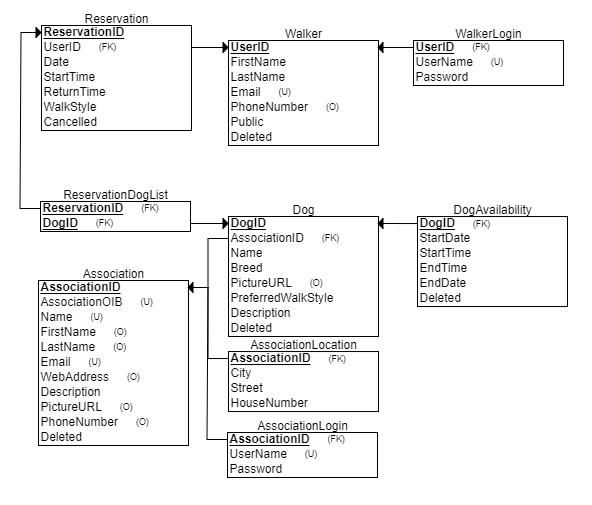
\includegraphics[scale=1.2]{dijagrami/database-scheme.png}
    			    \centering
    			    \caption{Dijagram baze podataka}
    			    \label{fig:shema}
		        \end{figure}
			
			\eject
			
			
		\section{Dijagram razreda}
		
			Dijagrami razreda omogućavaju pojednostavljen pogled i lakše razumijevanje komponenti arhitekture objektno orijentiranog sustava. Razredi sustava izrađenih u Springu prate norme razvojnog okvira. U našem sustavu zato imamo četiri glavna paketa i odgovarajuće potpakete. Njihov sadržaj moguće je vidjeti na sljedećim slikama:
			
			\begin{packed_item}
				\item[$\bullet$]  \textbf{domain} - Slika \ref{fig:classdiagram-domain}
				\item[$\bullet$]  \textbf{repository} - Slike \ref{fig:classdiagram-repository} i \ref{fig:classdiagram-repository-jpa}
				\item[$\bullet$]  \textbf{service} - Slika \ref{fig:classdiagram-service}
				    \begin{itemize}
				            \item[$\bullet$] \textbf{impl} - Slika \ref{fig:classdiagram-service-impl}
				    \end{itemize}
				\item[$\bullet$]  \textbf{rest} - Slika \ref{fig:classdiagram-rest}
				    \begin{itemize}
				        \item[$\bullet$] \textbf{dto} - Slika \ref{fig:classdiagram-rest-dto}
				    \end{itemize}
			\end{packed_item} 
			
			
			\begin{figure}[H]
    			    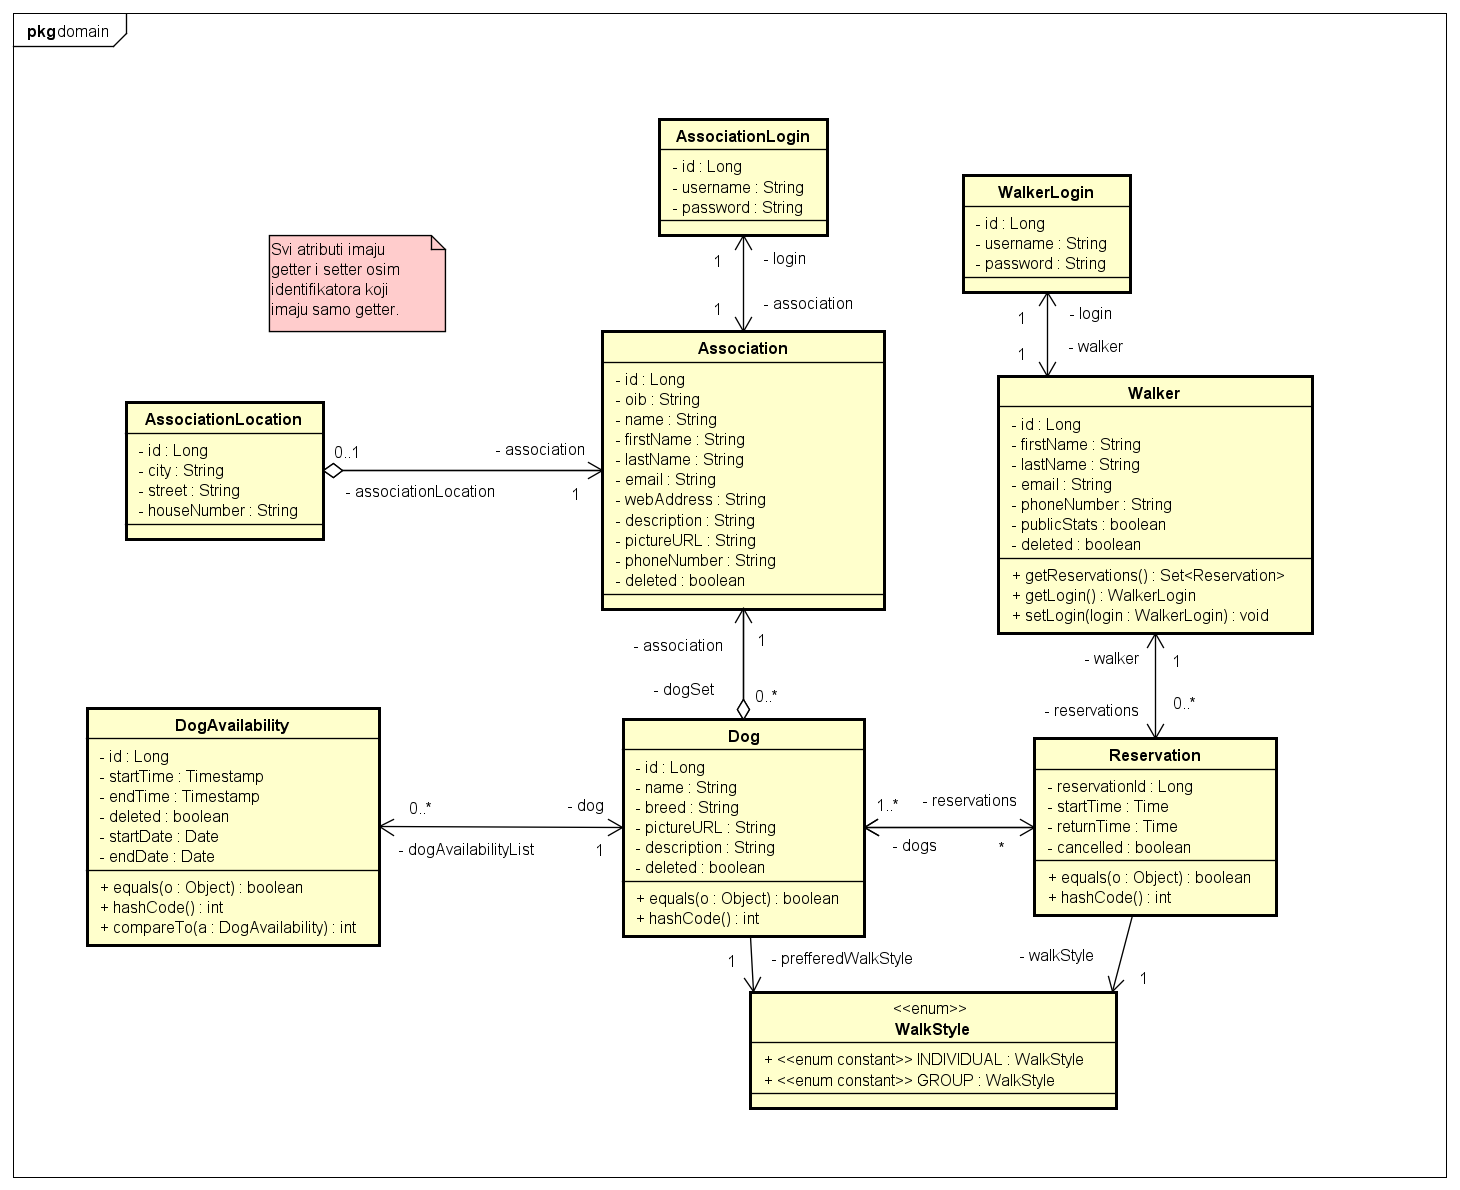
\includegraphics[scale=0.38]{dijagrami/classdiagram-domain.png}
    			    \centering
    			    \caption{Dijagram domenskih razreda}
    			    \label{fig:classdiagram-domain}
		    \end{figure}
		    
		    \noindent Na dijagramima je moguće vidjeti da kod prati načela troslojne arhitekture navedena na početku poglavlja. Klase paketa \textit{repository} služe za spremanje i dohvaćanje podataka iz baze pri čemu Spring nudi gotovo rješenje većine komunikacije s bazom u obliku JPA repozitorija (engl. \textit{Java Persistence API}). Repozitoriji našeg koda nasljeđuju JPA repozitorije kao što je moguće vidjeti na slici \ref{fig:classdiagram-repository-jpa}.
		    
		    \begin{figure}[H]
    			    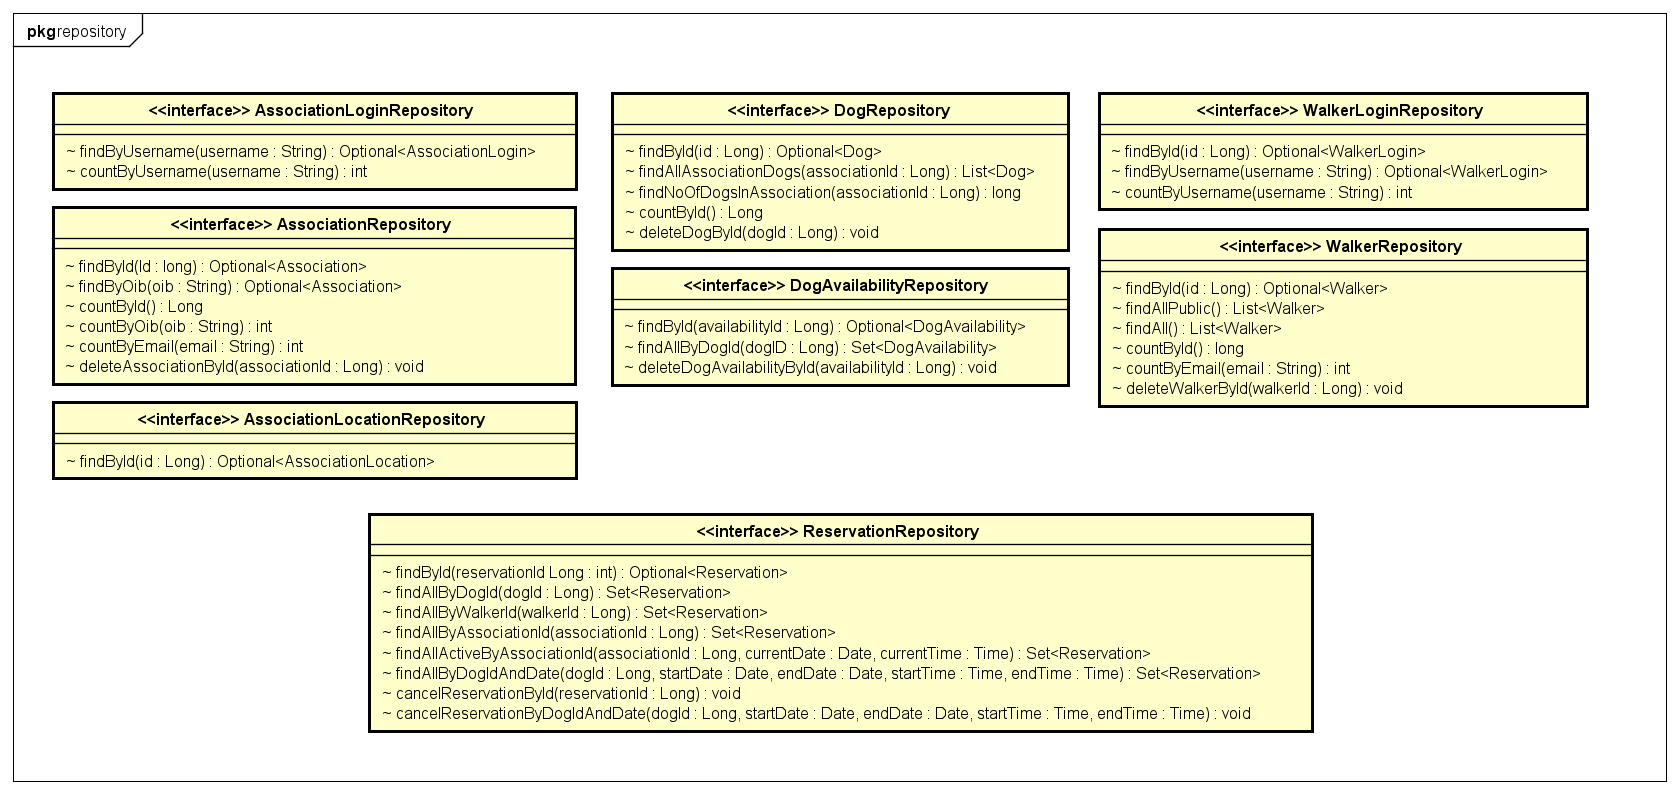
\includegraphics[scale=0.34]{dijagrami/classdiagram-repository.png}
    			    \centering
    			    \caption{Dijagram spremišnih razreda}
    			    \label{fig:classdiagram-repository}
		    \end{figure}
		    
		    
		    
		     \begin{figure}[H]
    			    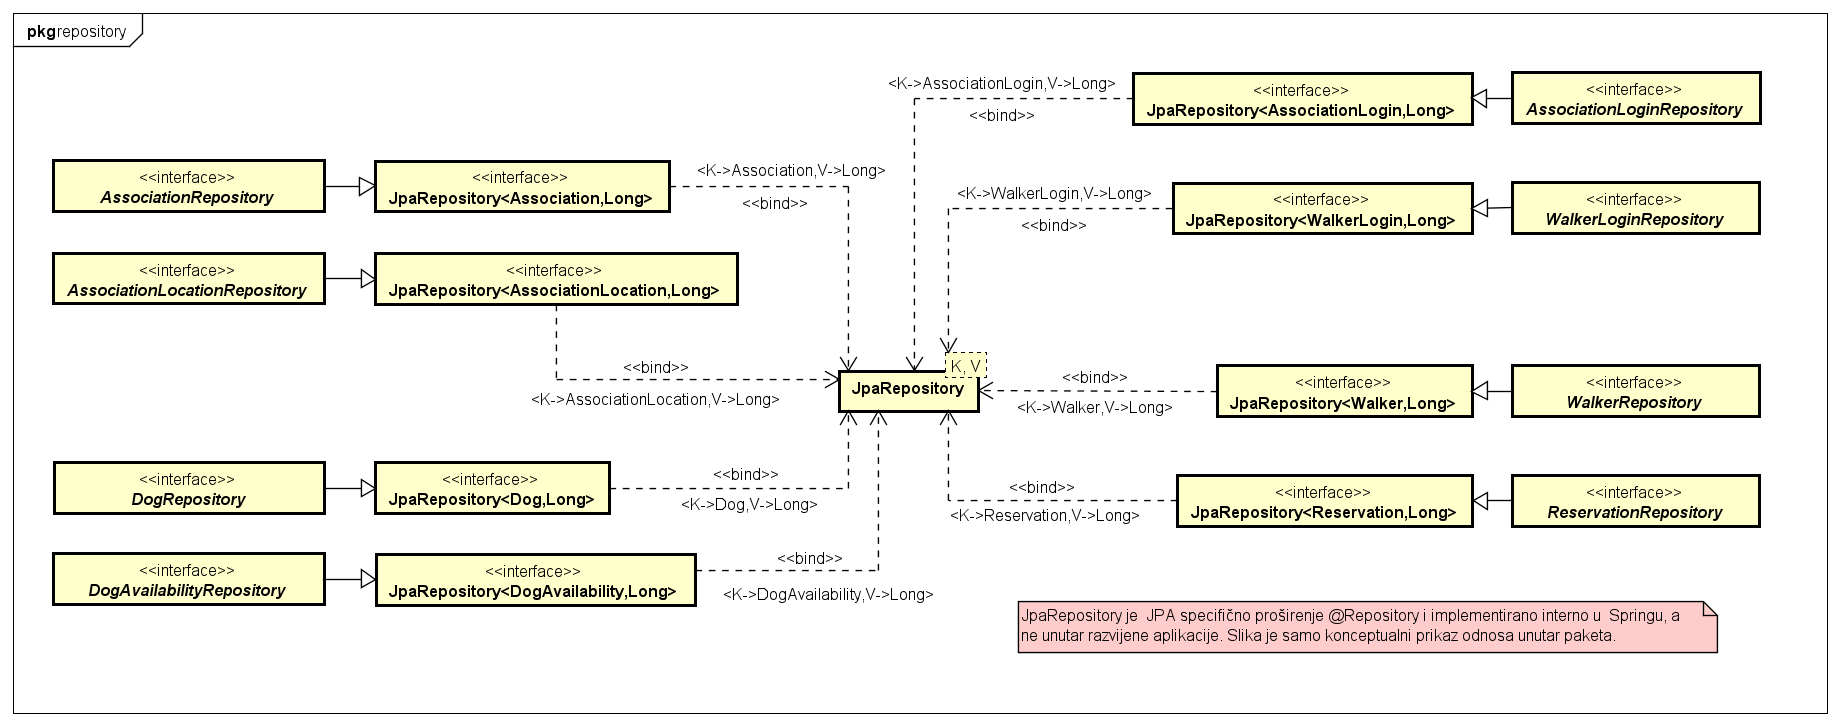
\includegraphics[scale=0.31]{dijagrami/classdiagram-repository-jpa.png}
    			    \centering
    			    \caption{Nasljeđivanje JPA repozitorija}
    			    \label{fig:classdiagram-repository-jpa}
		    \end{figure}
		    
		    \bigskip
		    \noindent Paket \textit{service} sadrži sučelja koja definiraju funkcionalnosti servisnog sloja. Ona se ostvaruju u potpaketu \textit{impl}. Implementacijske klase sadrže reference na potrebne repozitorije kako bi mogle dohvaćati i spremati podatke te manipulirati njima.
		    
		    \begin{figure}[H]
    			    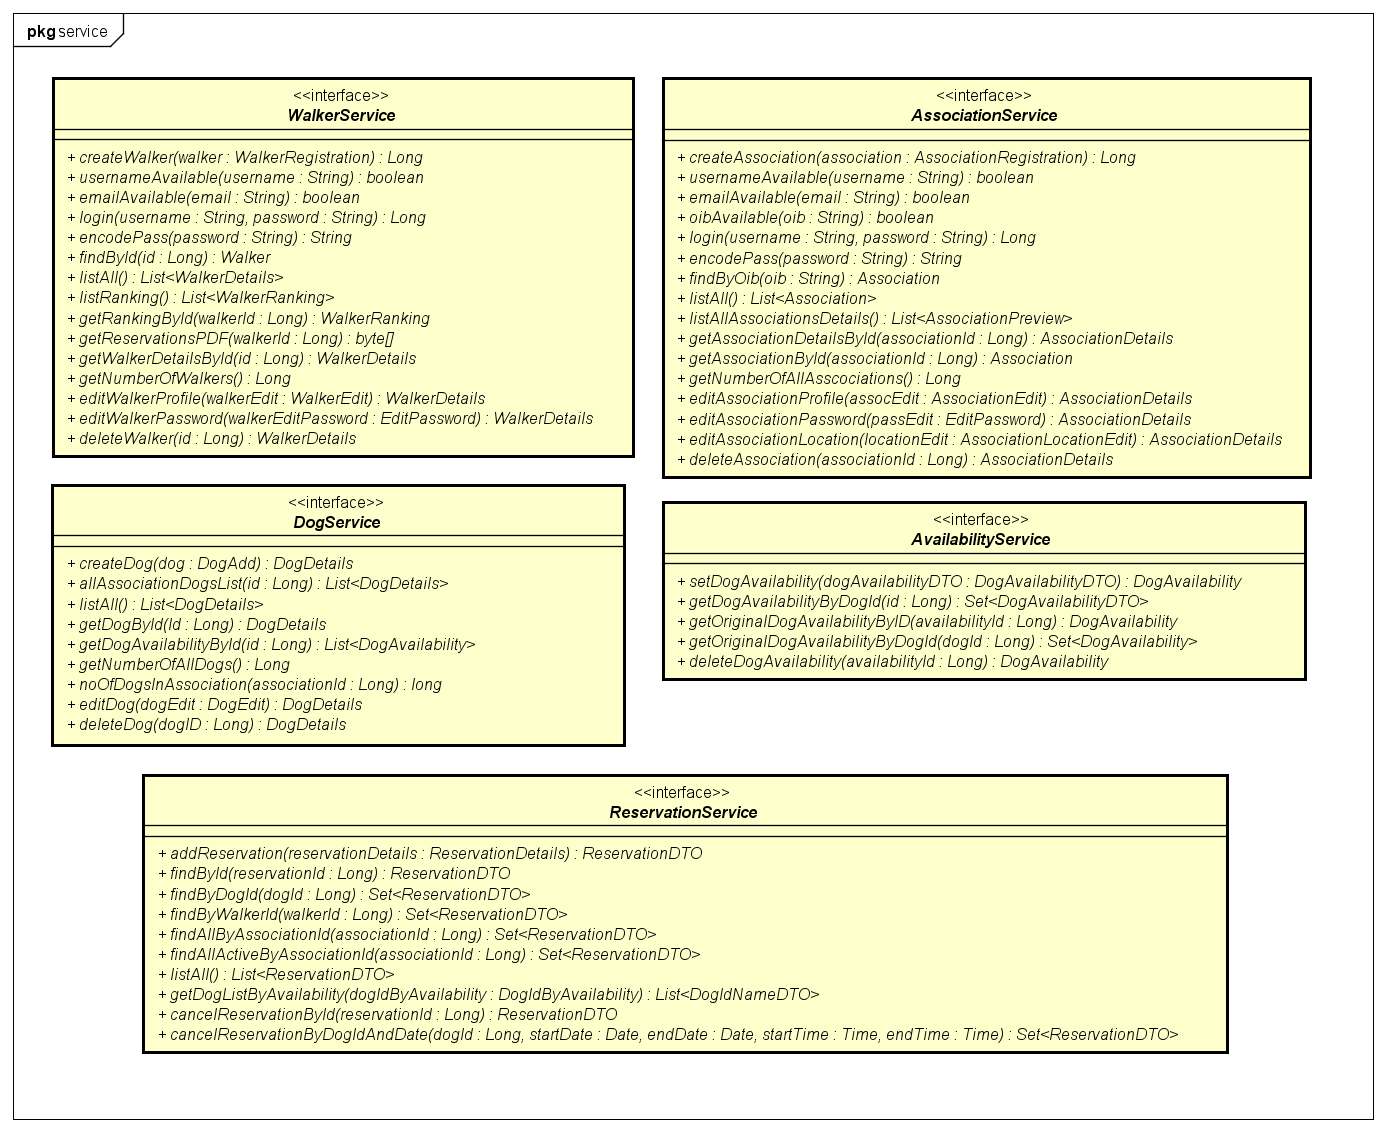
\includegraphics[scale=0.27]{dijagrami/classdiagram-service.png}
    			    \centering
    			    \caption{Dijagram servisnih sučelja}
    			    \label{fig:classdiagram-service}
		    \end{figure}
		    
		    \begin{figure}[H]
    			    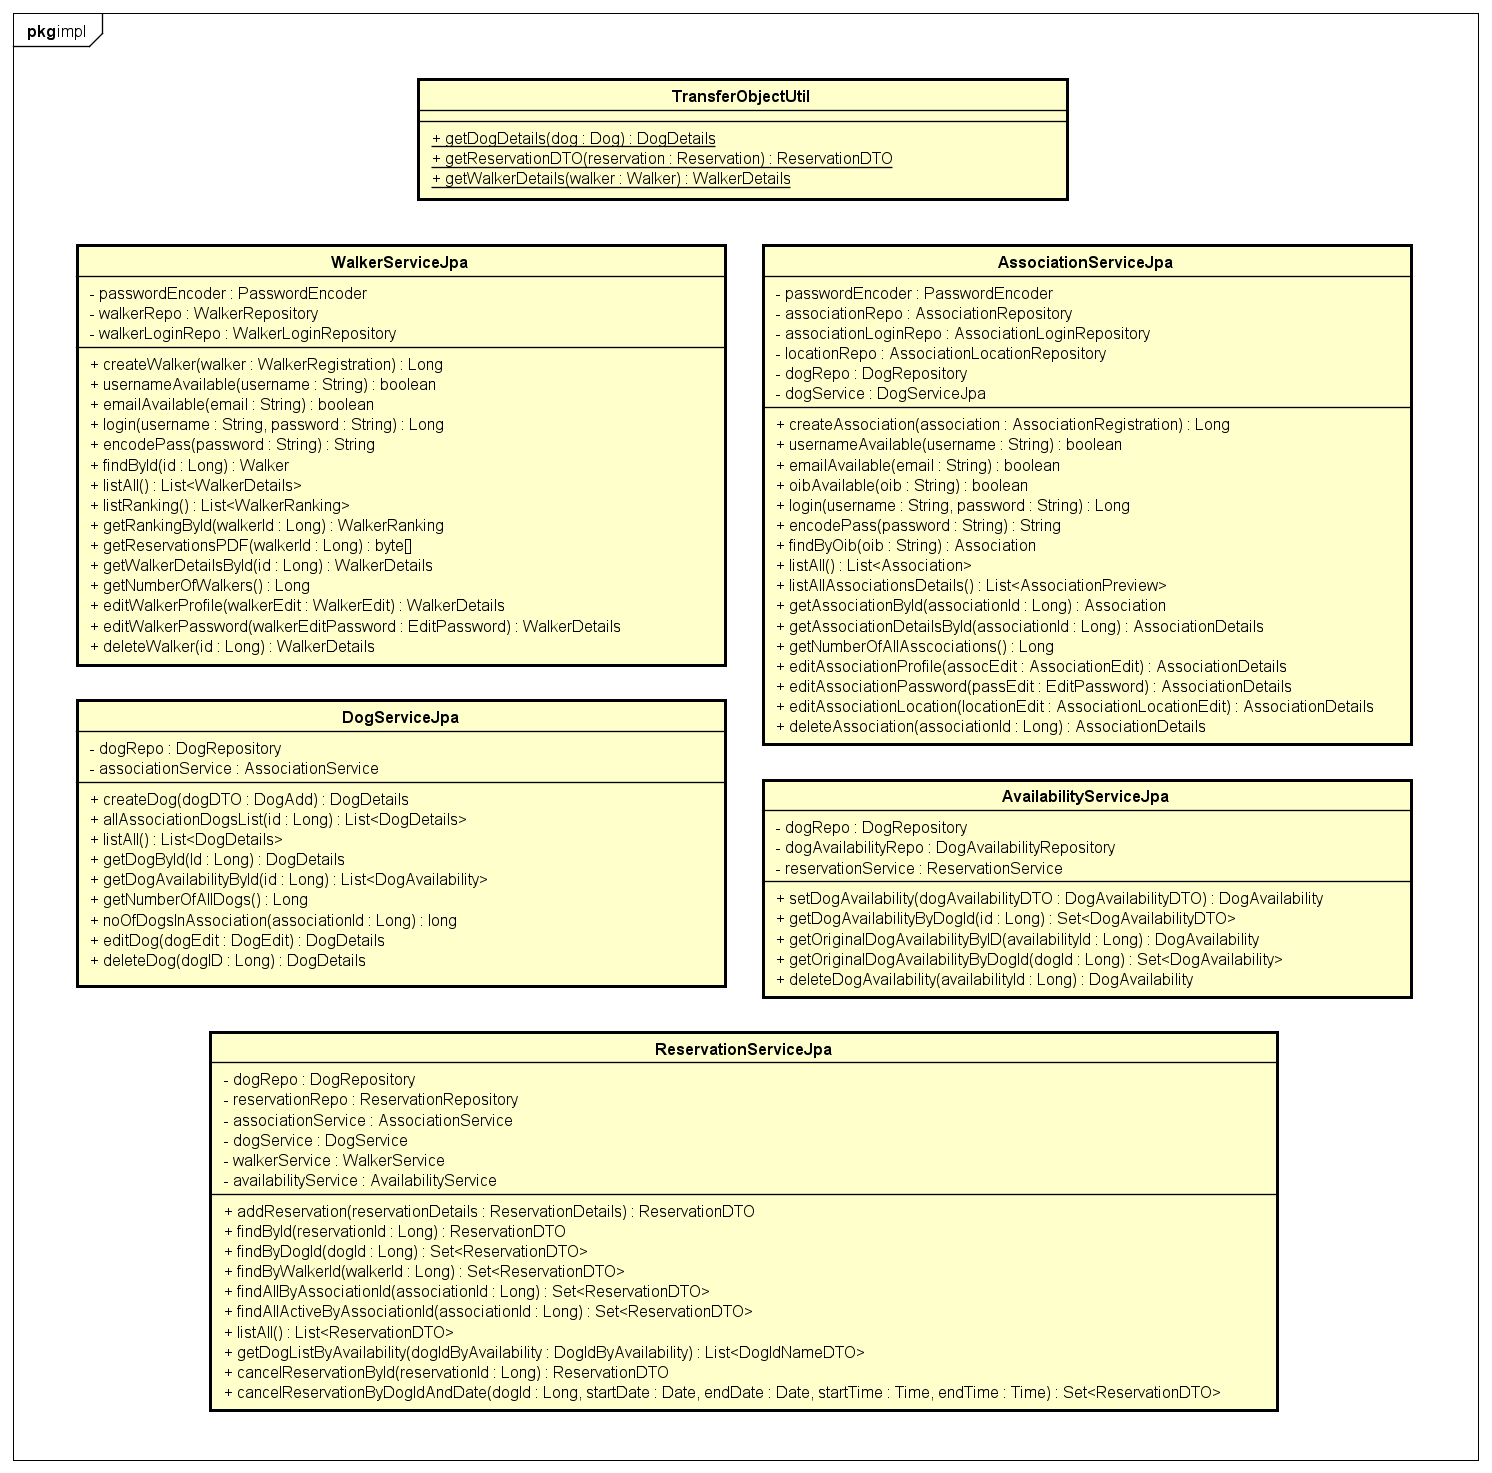
\includegraphics[scale=0.32]{dijagrami/classdiagram-service-impl.png}
    			    \centering
    			    \caption{Dijagram razreda implementacije servisnih sučelja}
    			    \label{fig:classdiagram-service-impl}
		    \end{figure}
		    
		    \noindent Razredi paketa \textit{rest} komuniciraju s \textit{frontend} stranom razvijenog sustava i nazivaju se i kontrolerima. Razmijenjuju informacije u formatu JSON i odgovarajućim HTTP status kodom. Za formatiranje odgovora koriste se razredima paketa DTO (engl. \textit{Data Transfer Object}). Sadrže reference na servisna sučelja kojima dohvaćaju obrađene podatke ili ih šalju na obradu.
		    
		    \bigskip
		    
		    \begin{figure}[H]
    			    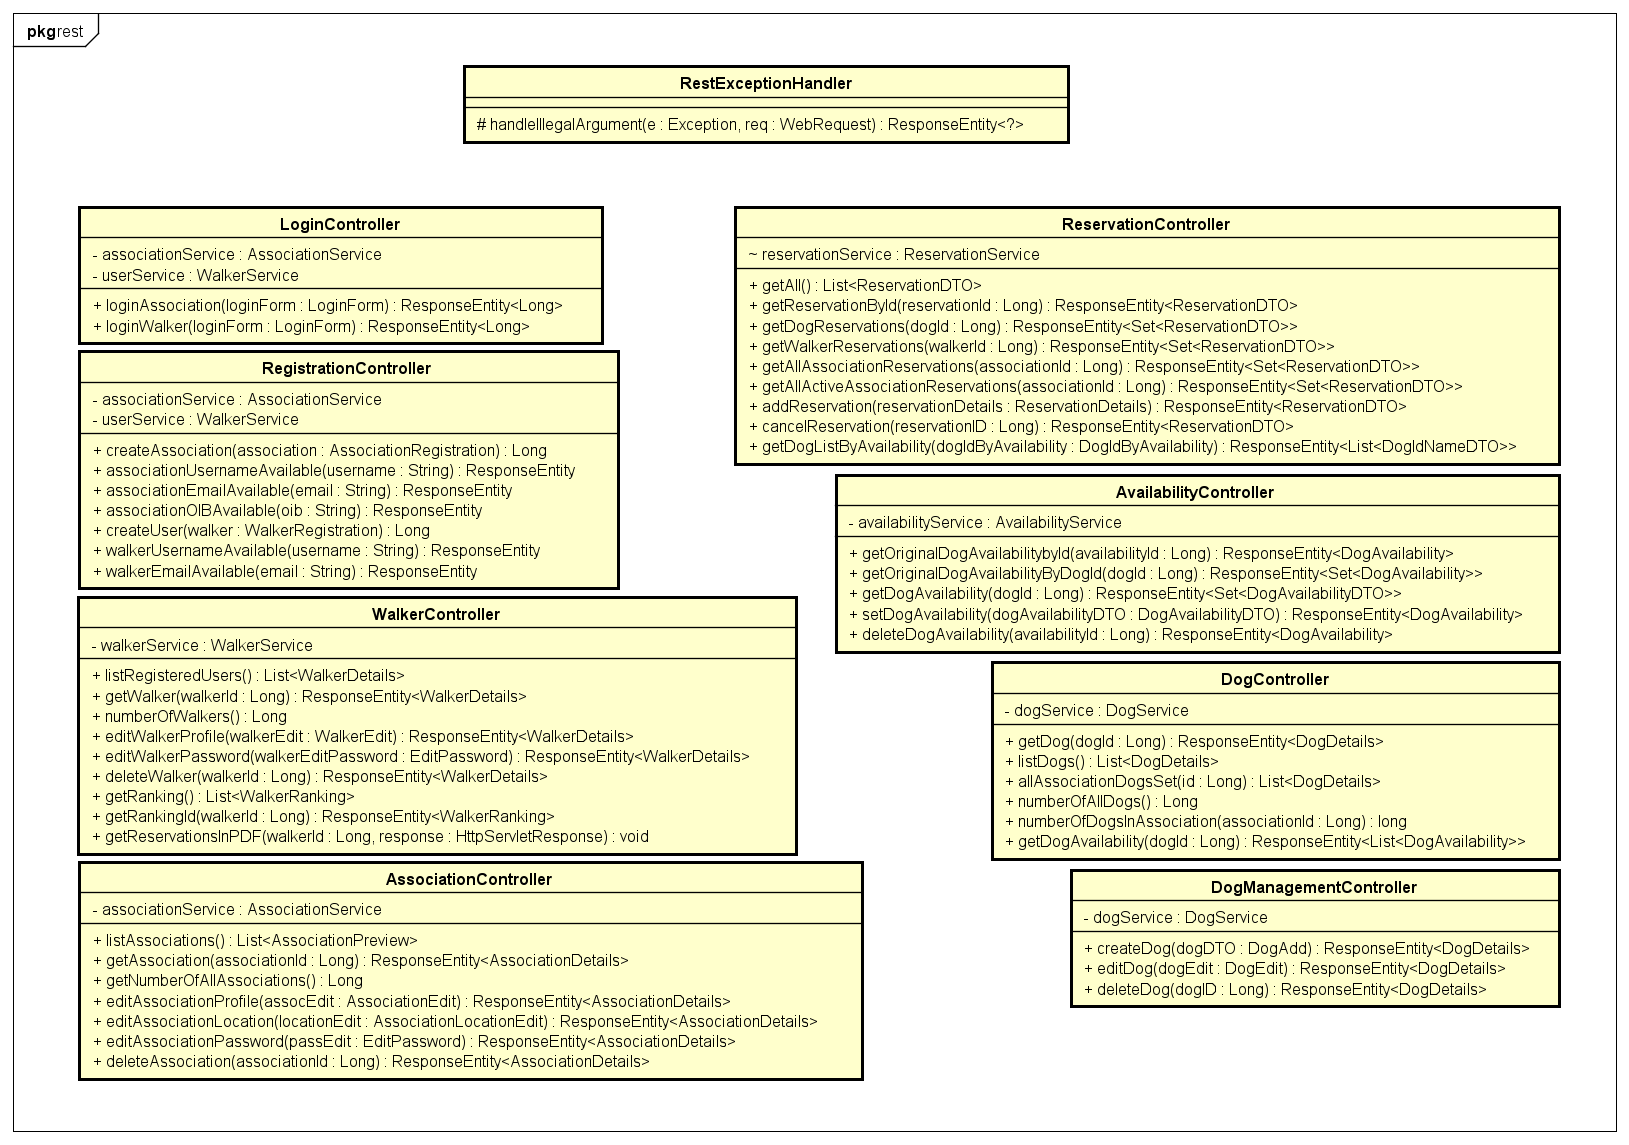
\includegraphics[scale=0.35]{dijagrami/classdiagram-rest.png}
    			    \centering
    			    \caption{Dijagram razreda kontrolera}
    			    \label{fig:classdiagram-rest}
		    \end{figure}
		    
		    \bigskip
		    
		    \noindent Na slici \ref{fig:classdiagram-doggo} moguće je vidjeti ishodišni razred cijele aplikacije \textit{DogGoApplication} i razred konfiguracije dozvoljenih HTTP zahtjeva u aplikaciji koji nasljeđuje već gotovi razred Spring razvojnog okvira \textit{WebMvcConfigurer}.
		    
		    \bigskip
		    
		     \begin{figure}[H]
    			    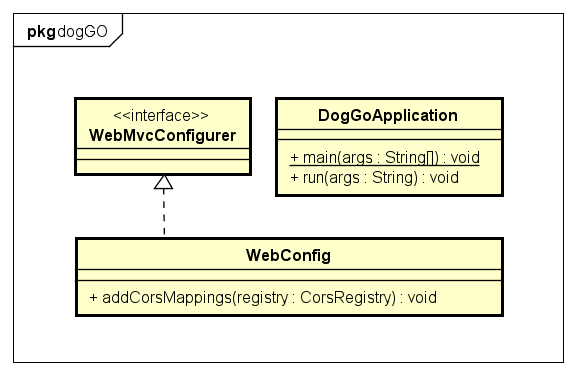
\includegraphics[scale=0.35]{dijagrami/classdiagram-doggo.png}
    			    \centering
    			    \caption{Ishodišni paket aplikacije}
    			    \label{fig:classdiagram-doggo}
		    \end{figure}
		    
		    \begin{figure}[H]
    			    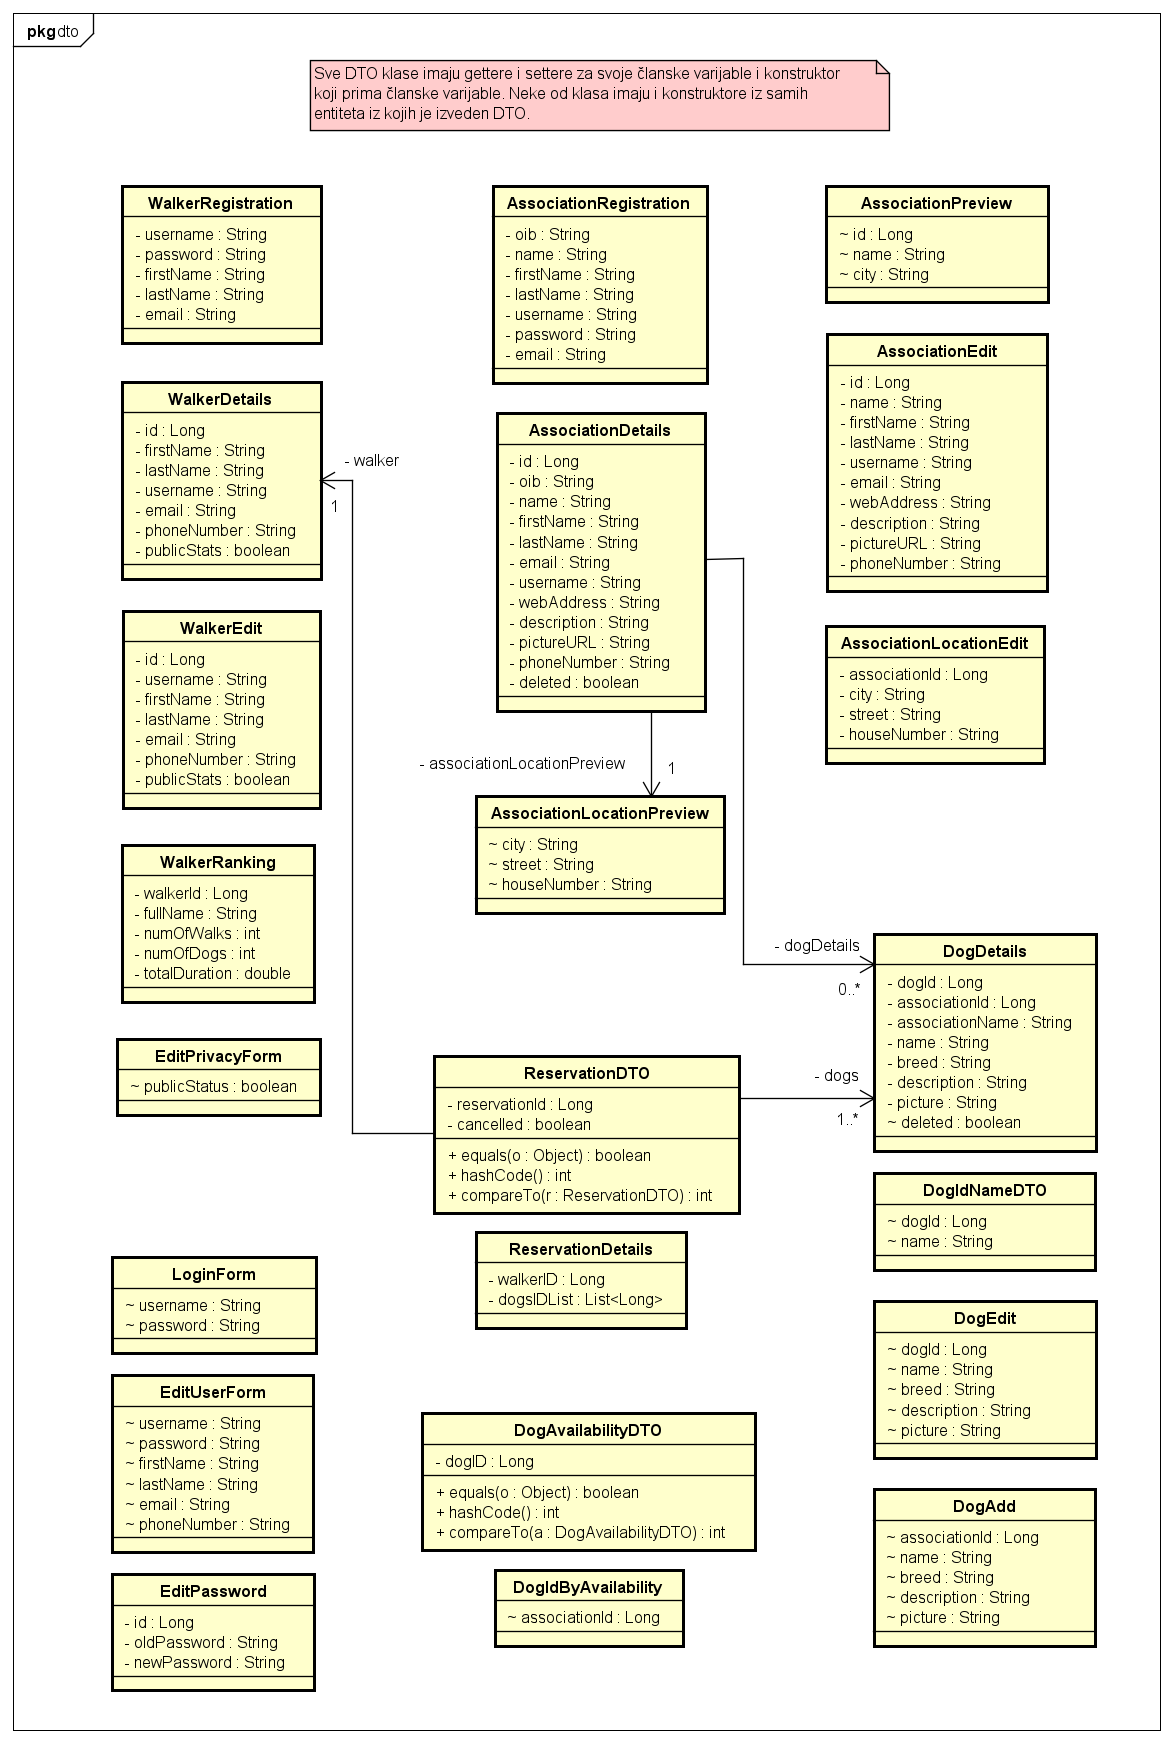
\includegraphics[scale=0.47]{dijagrami/classdiagram-rest-dto.png}
    			    \centering
    			    \caption{Dijagram razreda objekata prijenosa podataka}
    			    \label{fig:classdiagram-rest-dto}
		    \end{figure}
			
			\eject
		
		\section{Dijagram stanja}
			
			Dijagram stanja prikazuje stanja objekata te prijelaze iz jednog u drugo stanje na temelju događaja.
Na slici \ref{fig:states} je prikazan dijagram stanja za registriranog šetača. 
Neregistriranom korisniku se prikazuje naslovna stranica. Od tamo, korisnik može pregledati javnu statistiku te može dobiti uvid u sve registrirane udruge i njihove profile gdje su prikazane informacije o njima i svim njihovim psima.
Nakon prijave korisnika kao šetača, korisnik dobiva mogućnost rezervacije šetnje odabranog psa u slobodnom terminu. Na stranici „Moj profil“ korisnik može urediti osobne podatke, pregledati kalendar rezerviranih šetnji te u obliku pdf-a skinuti vlastiti raspored nadolazećih šetnji te obrisati svoj profil.

    \begin{figure}[H]
    			    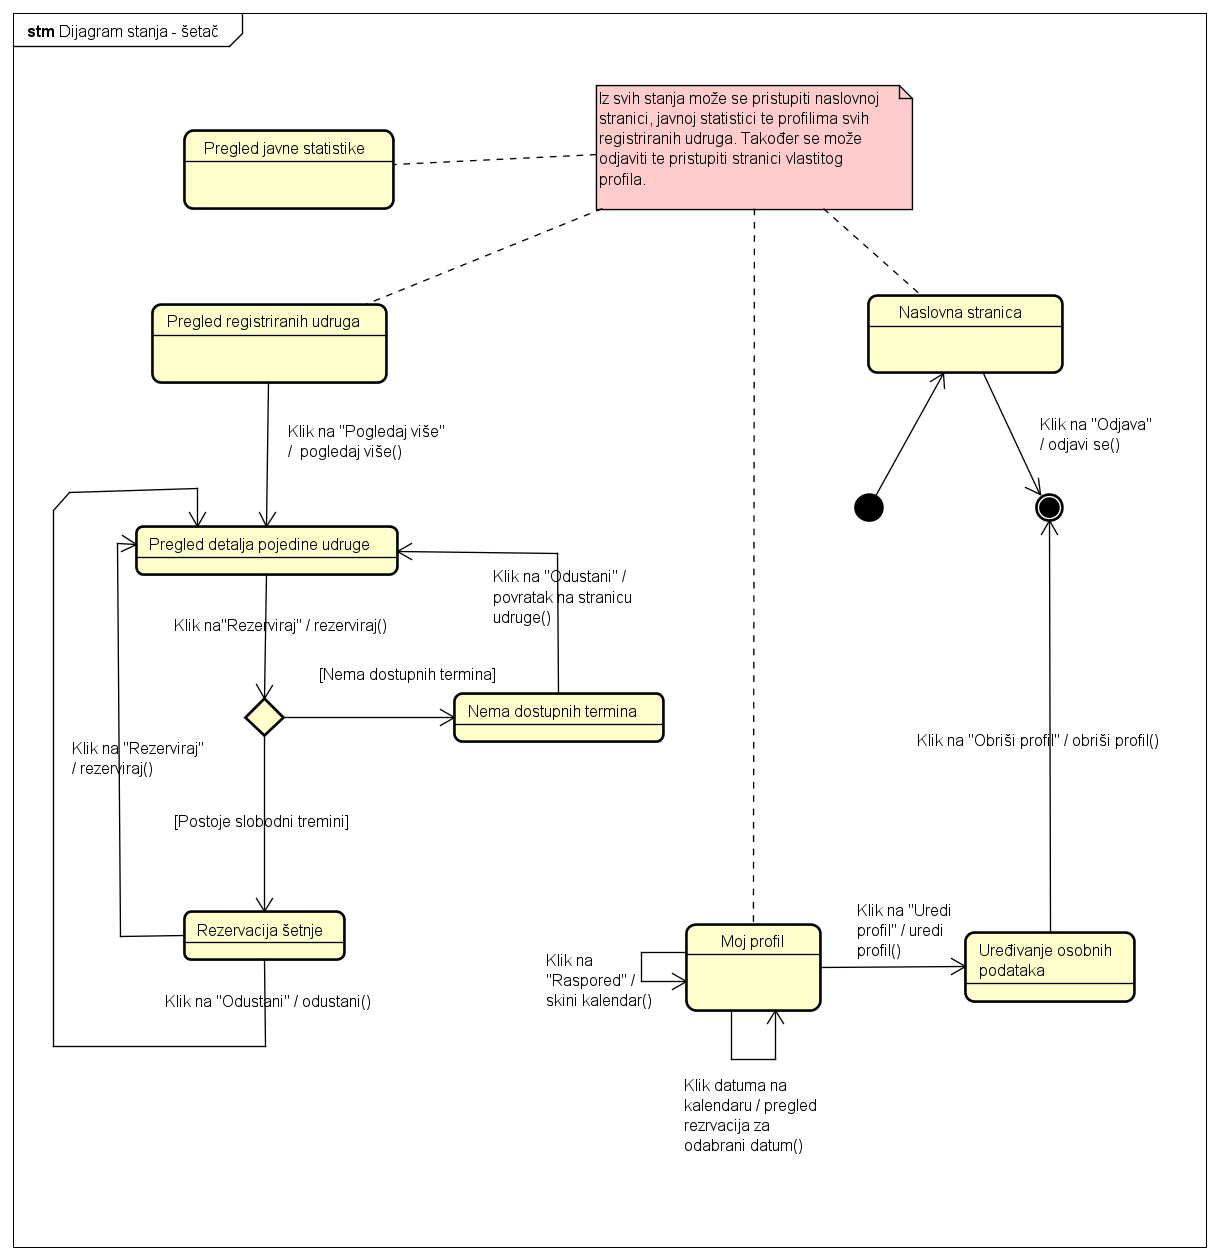
\includegraphics[scale=0.45]{dijagrami/Dijagram_stanja-setac.png}
    			    \centering
    			    \caption{Dijagram stanja}
    			    \label{fig:states}
		    \end{figure}
			
		
			\eject 
		
		\section{Dijagram aktivnosti}
			
			\begin{figure}[H]
			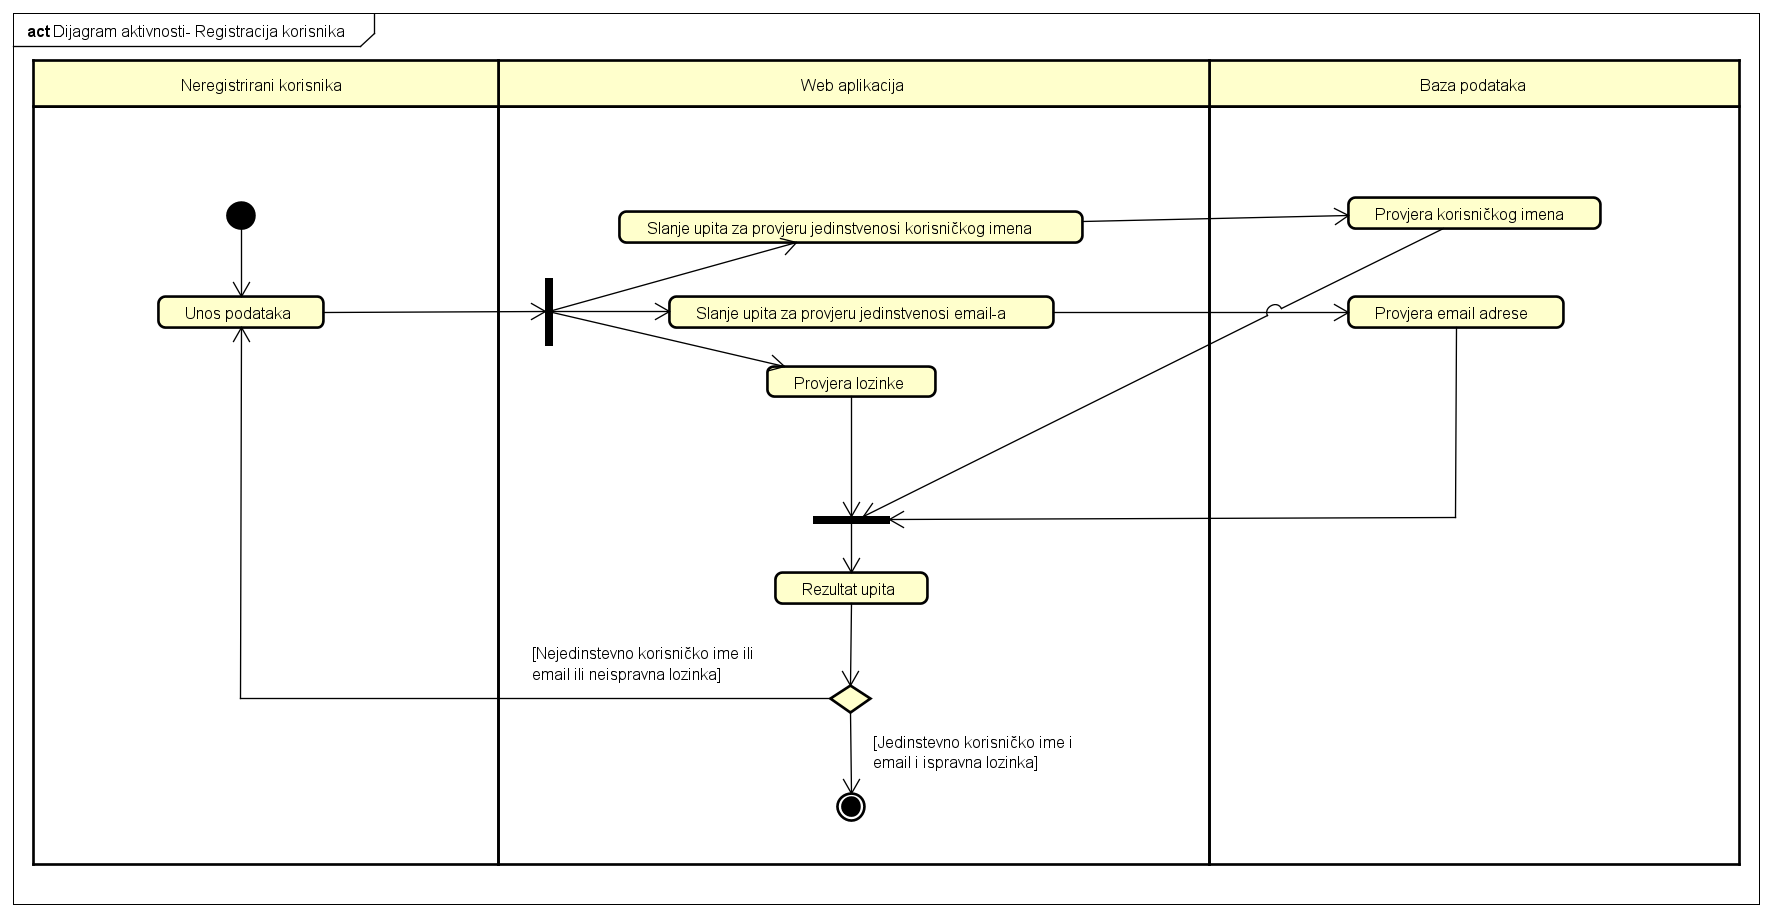
\includegraphics[scale=0.3]{dijagrami/Dijagram_aktivnosti-Registracija_korisnika.png}
			\centering
			\caption{Dijagram aktivnosti za registraciju korisnika}
			\label{fig:activity_diagram_1}
		\end{figure}	

		\begin{figure}[H]
			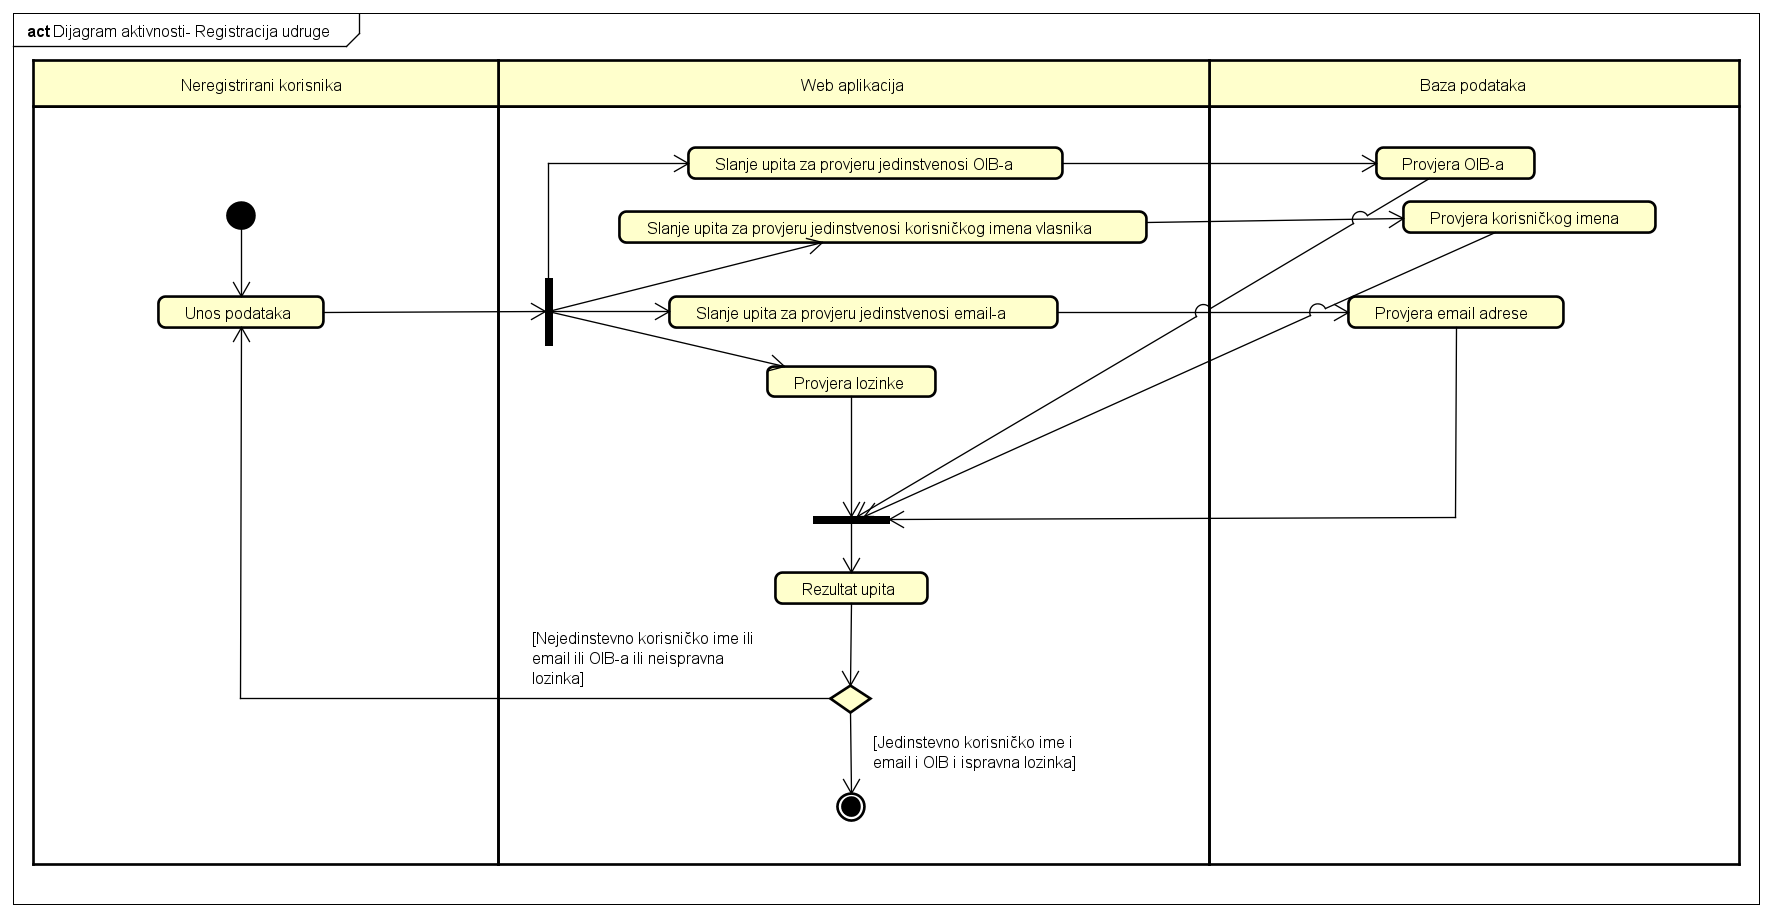
\includegraphics[scale=0.3]{dijagrami/Dijagram_aktivnosti-Registracija_udruge.png}
			\centering
			\caption{Dijagram aktivnosti za registraciju udruga}
			\label{fig:activity_diagram_2}
		\end{figure}	

		\begin{figure}[H]
			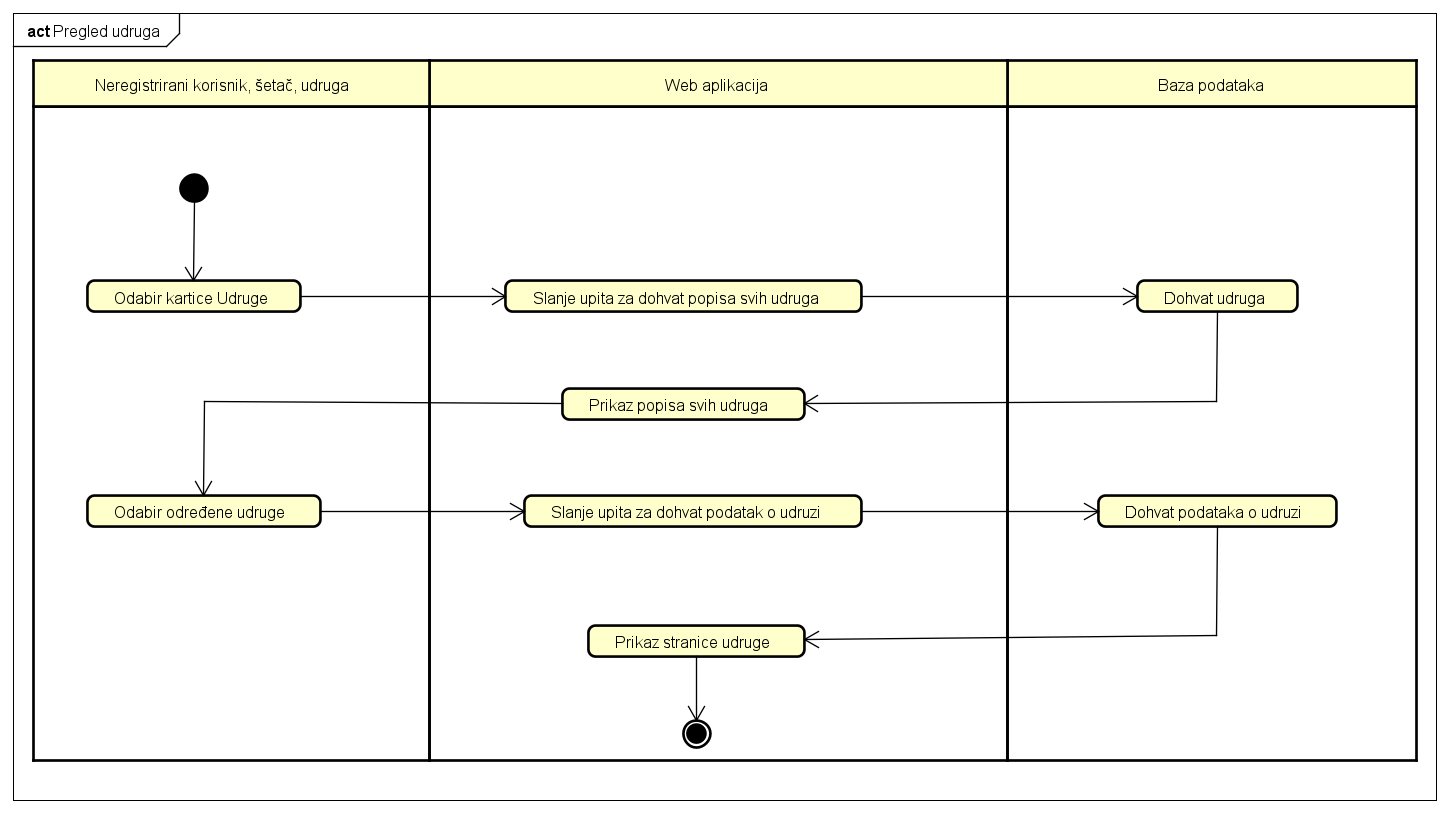
\includegraphics[scale=0.4]{dijagrami/Pregled_udruga.png}
			\centering
			\caption{Dijagram aktivnosti za pregled svih udruga}
			\label{fig:activity_diagram_3}
		\end{figure}

		\begin{figure}[H]
			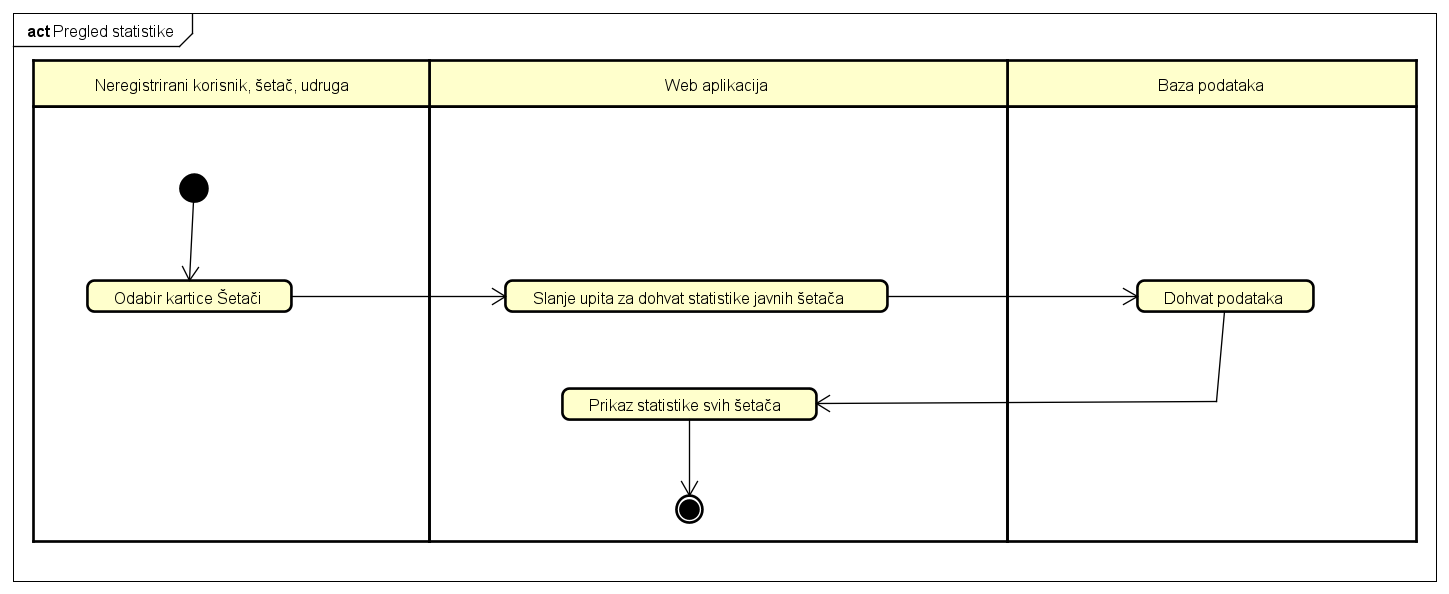
\includegraphics[scale=0.4]{dijagrami/Pregled_statistike.png}
			\centering
			\caption{Dijagram aktivnosti za pregled statistike šetača}
			\label{fig:activity_diagram_4}
		\end{figure}


		\begin{figure}[H]
			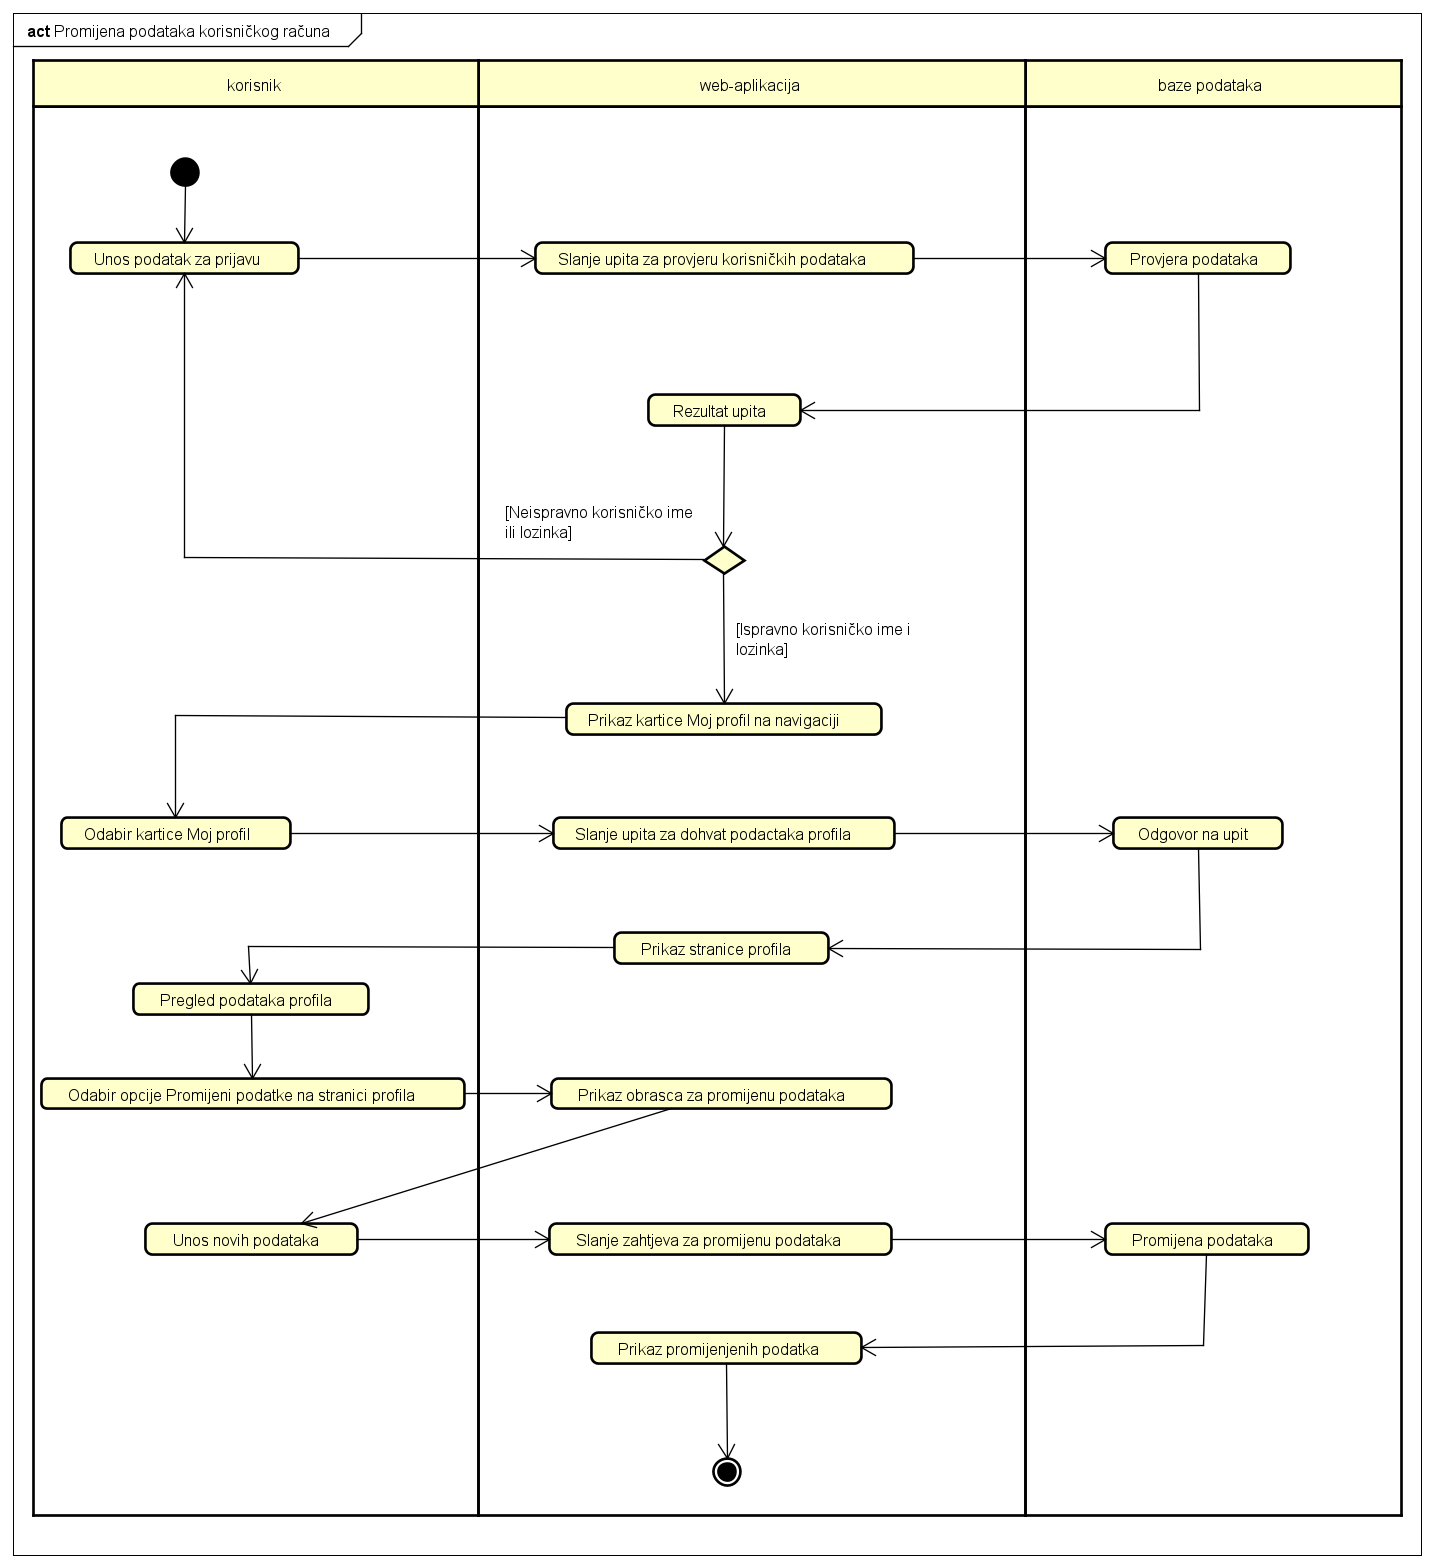
\includegraphics[scale=0.4]{dijagrami/Promijena_podataka_korisnickog_racuna.png}
			\centering
			\caption{Dijagram aktivnosti za promjenu podataka korisničkog računa}
			\label{fig:activity_diagram_5}
		\end{figure}


		\begin{figure}[H]
			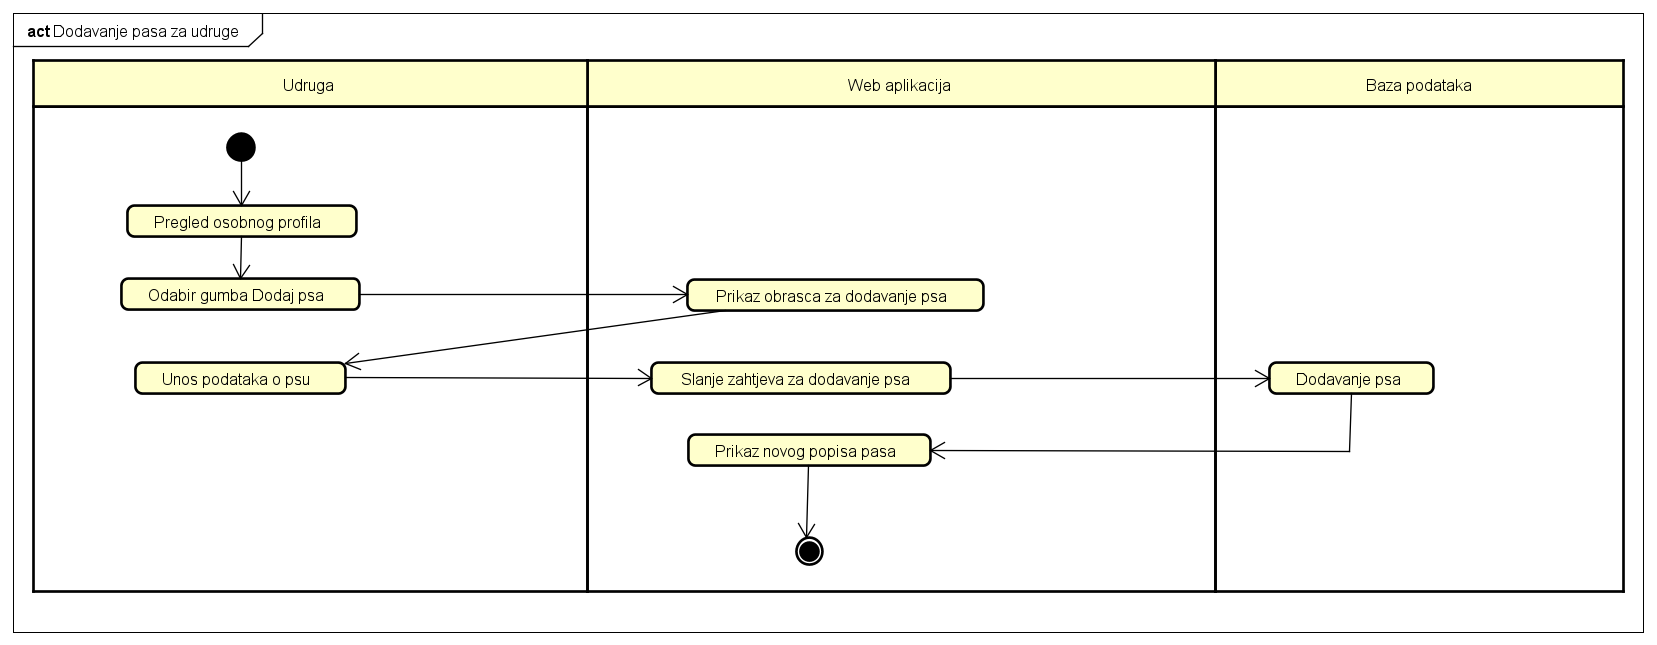
\includegraphics[scale=0.4]{dijagrami/Dodavanje_pasa_za_udruge.png}
			\centering
			\caption{Dijagram aktivnosti za dodavanje pasa kod udruga}
			\label{fig:activity_diagram_6}
		\end{figure}

		\begin{figure}[H]
			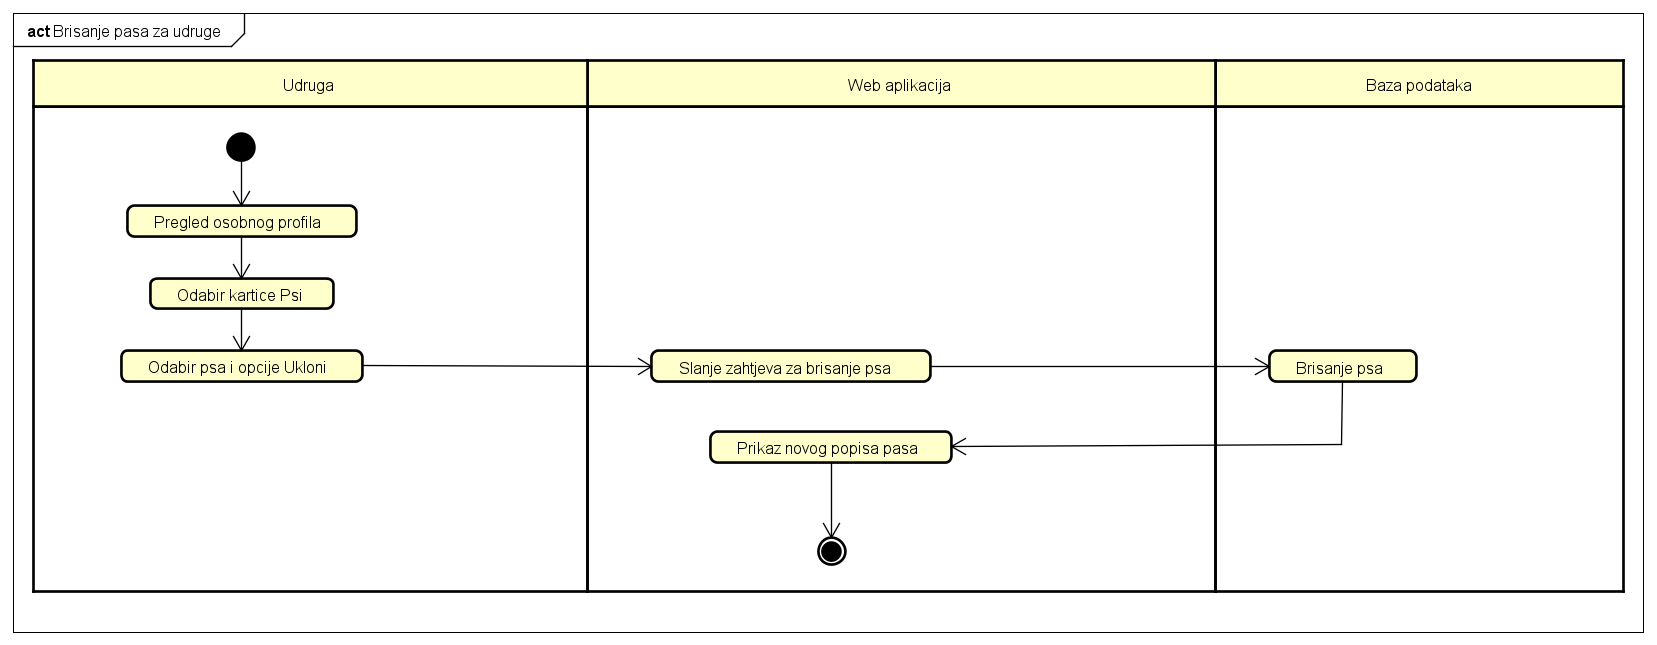
\includegraphics[scale=0.4]{dijagrami/Brisanje_pasa_za_udruge.png}
			\centering
			\caption{Dijagram aktivnosti za brisanje pasa kod udruga}
			\label{fig:activity_diagram_7}
		\end{figure}

		\begin{figure}[H]
			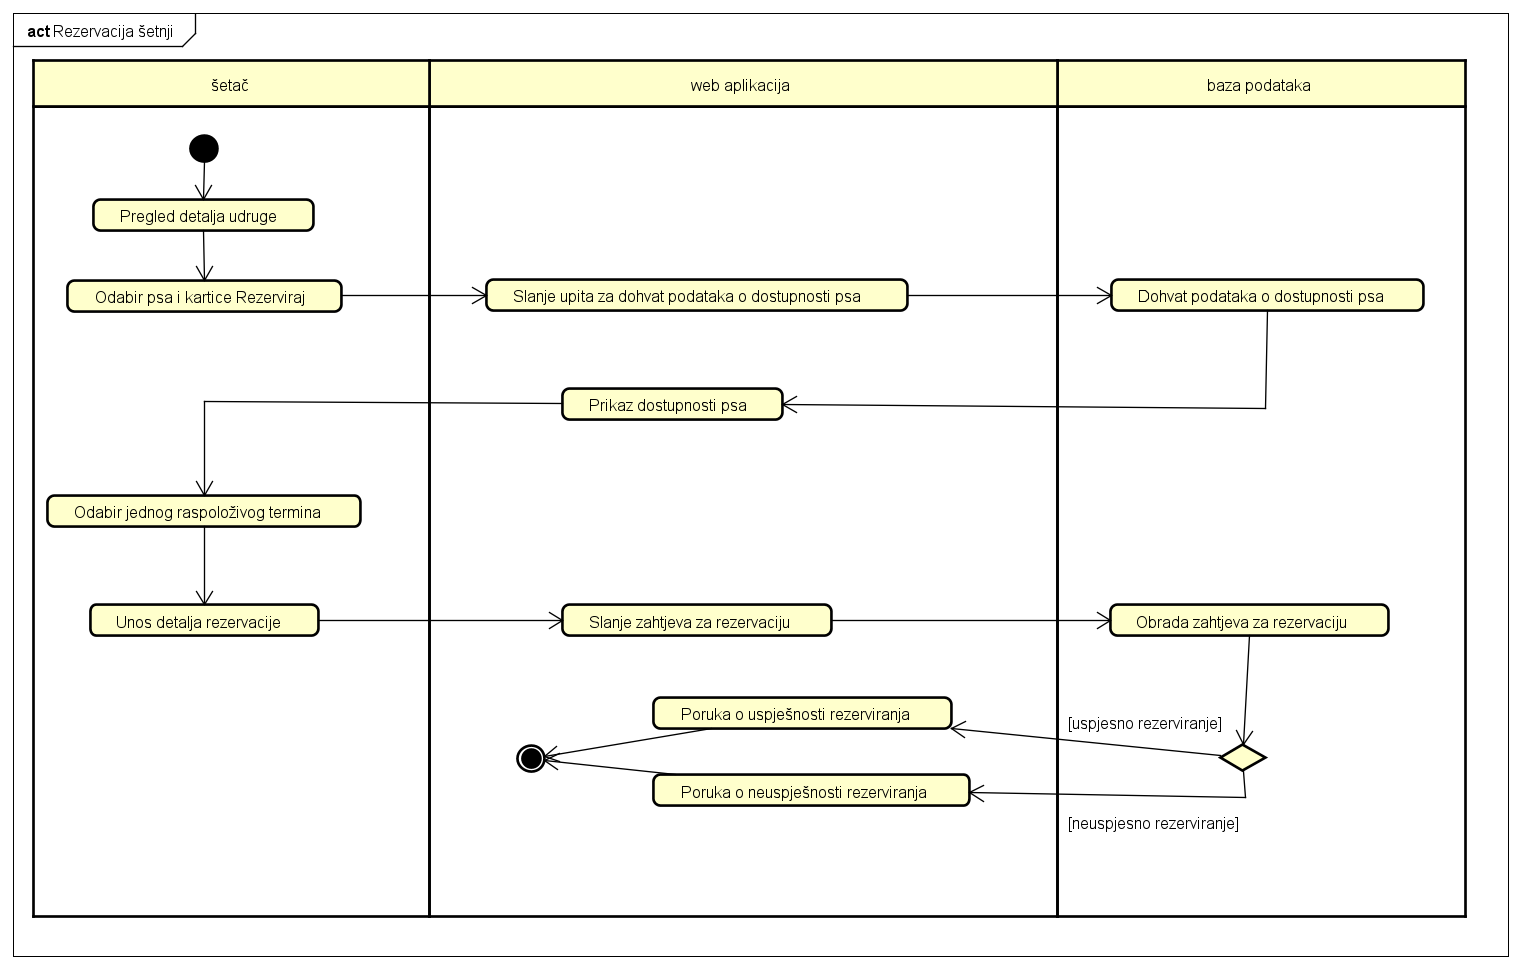
\includegraphics[scale=0.4]{dijagrami/Rezervacija_setnji.png}
			\centering
			\caption{Dijagram aktivnosti za rezervaciju šetnji}
			\label{fig:activity_diagram_8}
		\end{figure}

		\begin{figure}[H]
			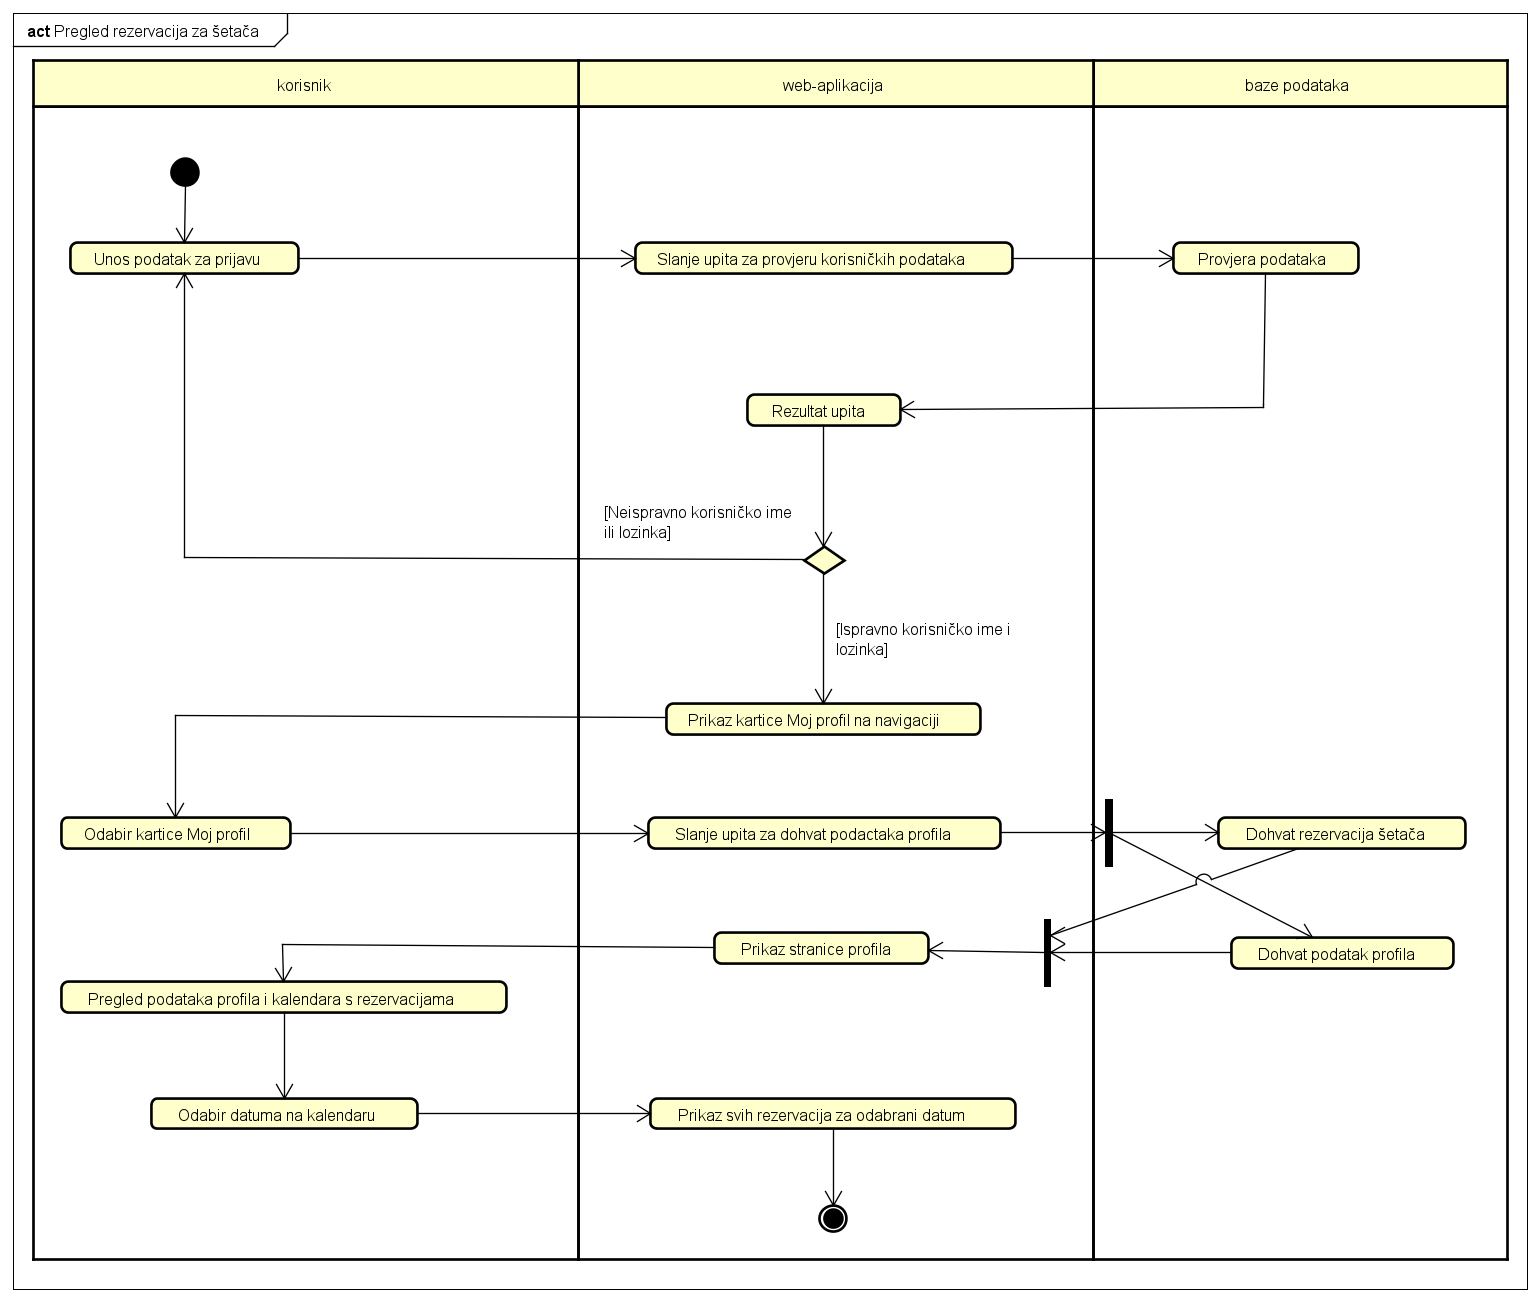
\includegraphics[scale=0.4]{dijagrami/Pregled_rezervacija_za_setaca.png}
			\centering
			\caption{Dijagram aktivnosti za pregled rezervacija šetača}
			\label{fig:activity_diagram_9}
		\end{figure}

		\begin{figure}[H]
			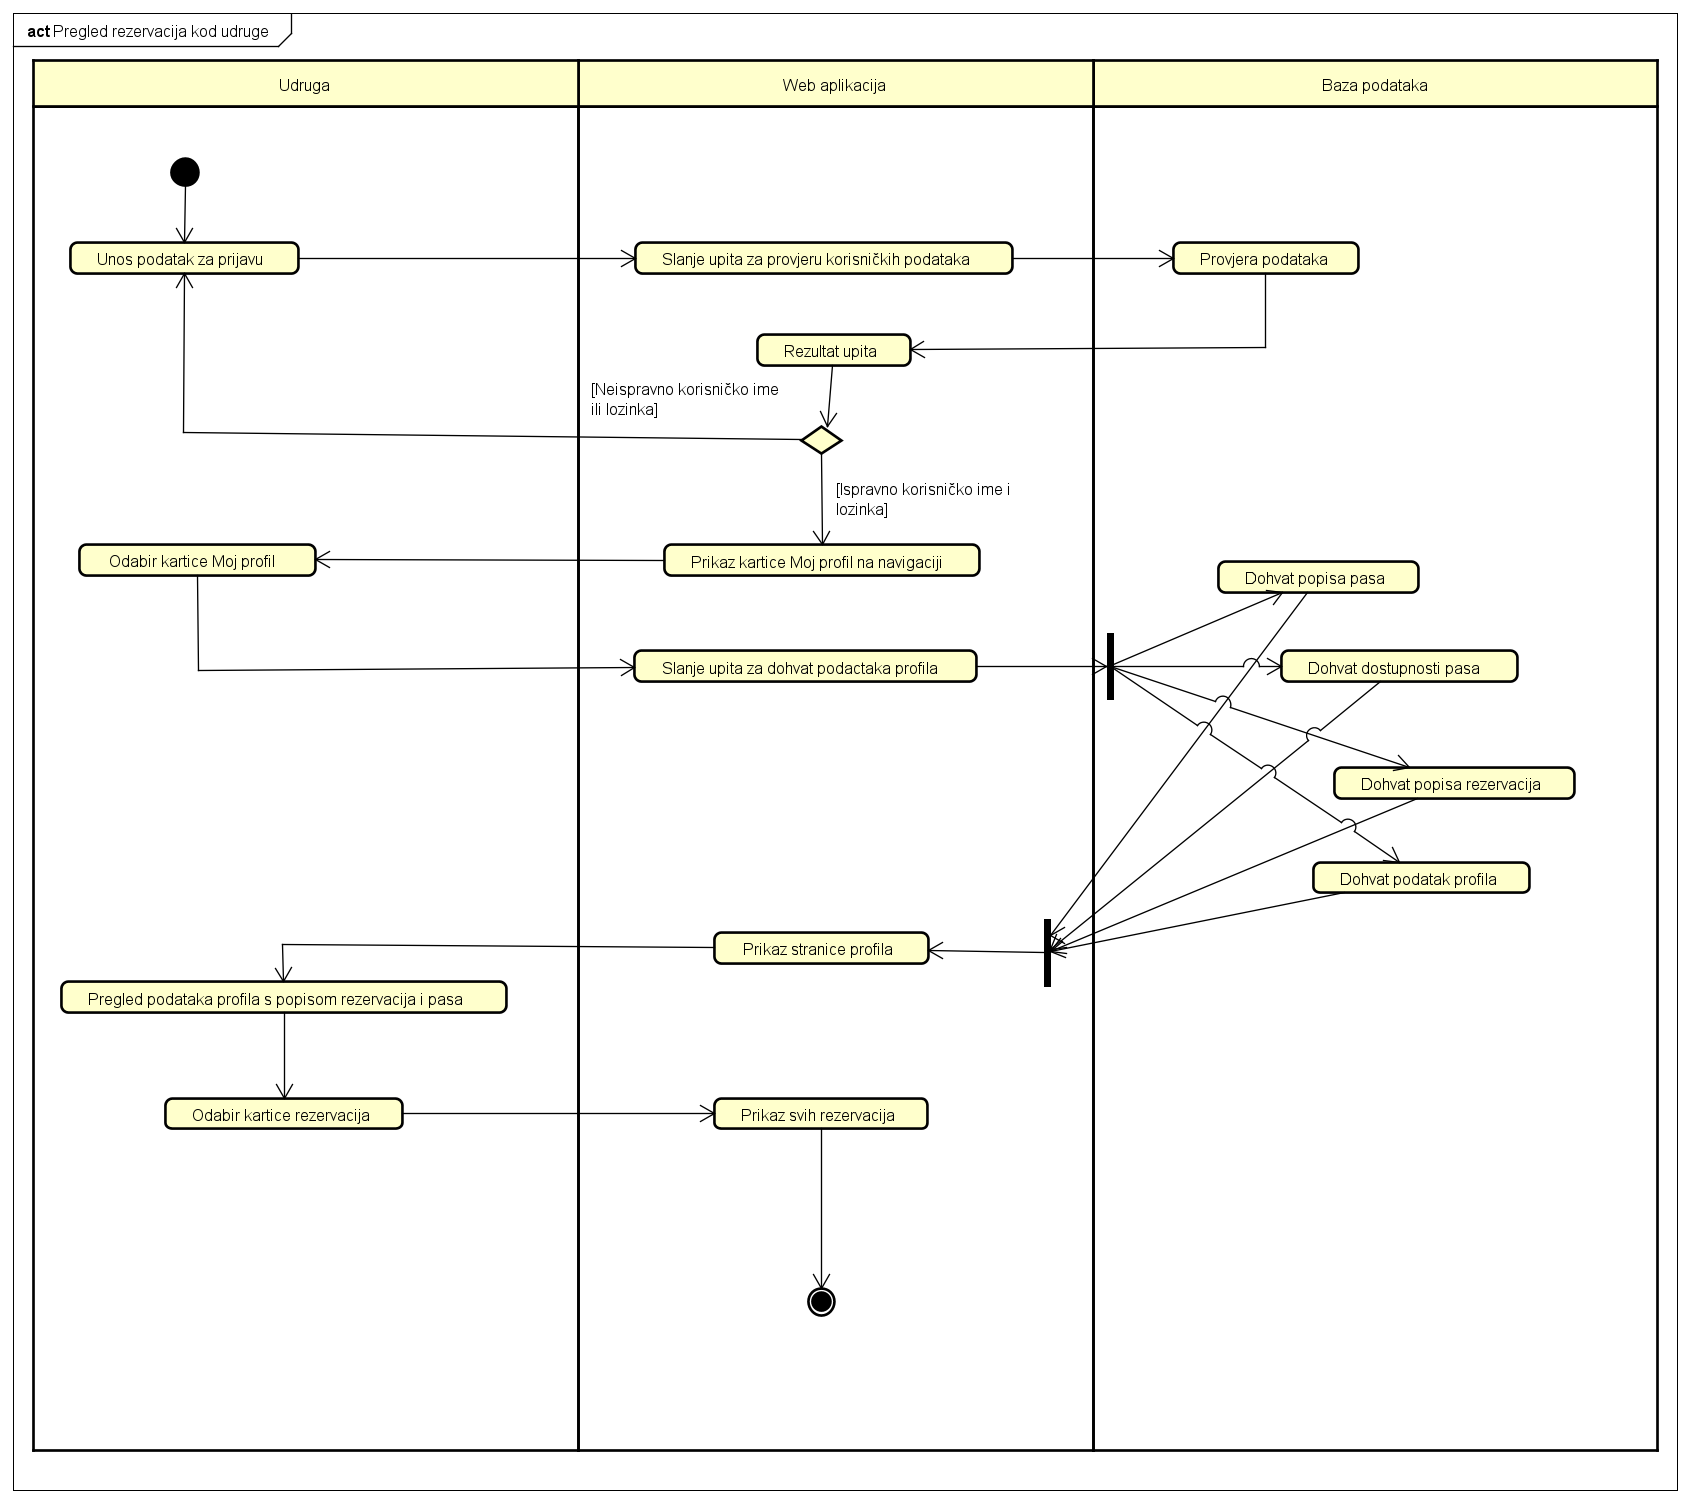
\includegraphics[scale=0.4]{dijagrami/Pregled_rezervacija_kod_udruge.png}
			\centering
			\caption{Dijagram aktivnosti za pregled rezervacija udruge}
			\label{fig:activity_diagram_10}
		\end{figure}

		\begin{figure}[H]
			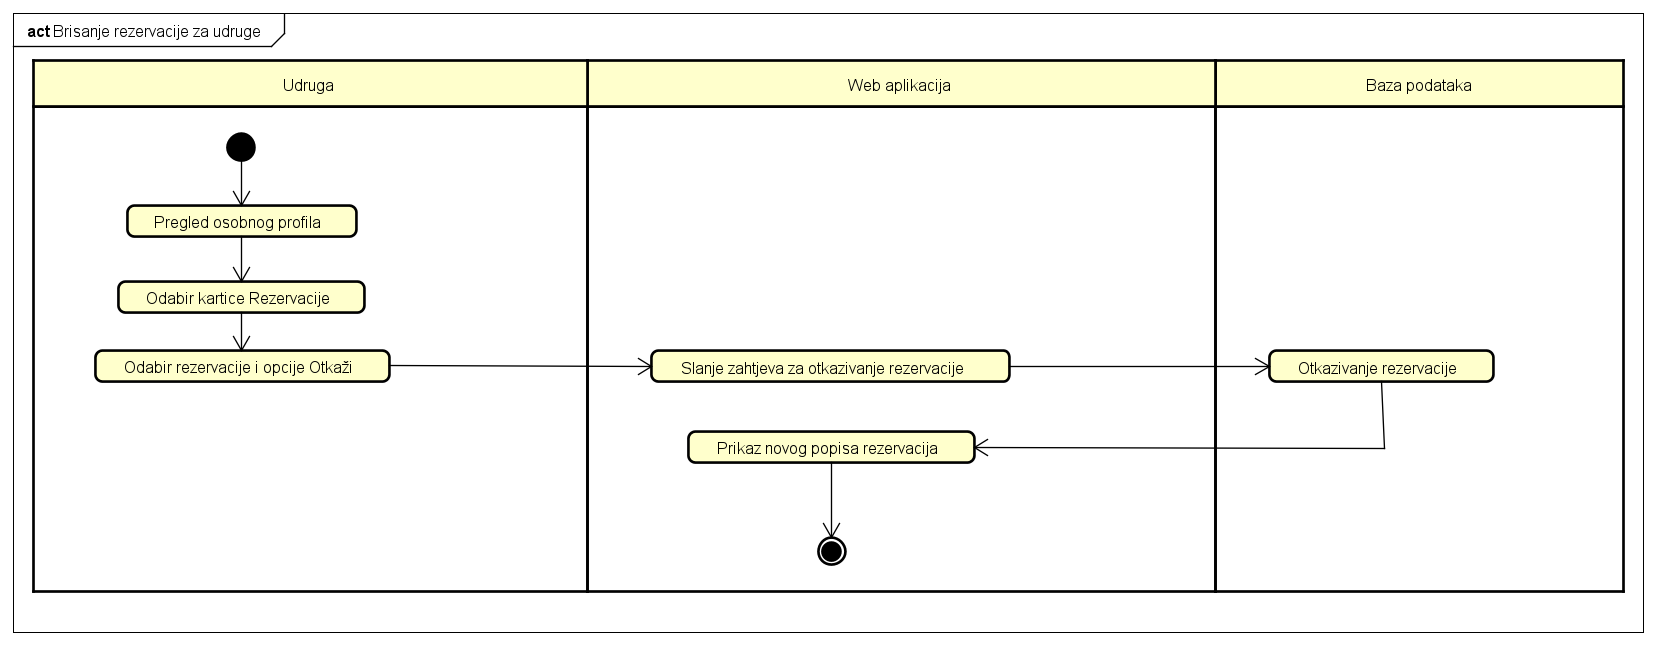
\includegraphics[scale=0.4]{dijagrami/Brisanje_rezervacije_za_udruge.png}
			\centering
			\caption{Dijagram aktivnosti za brisanje rezervacije kod udruge}
			\label{fig:activity_diagram_11}
		\end{figure}

		\begin{figure}[H]
			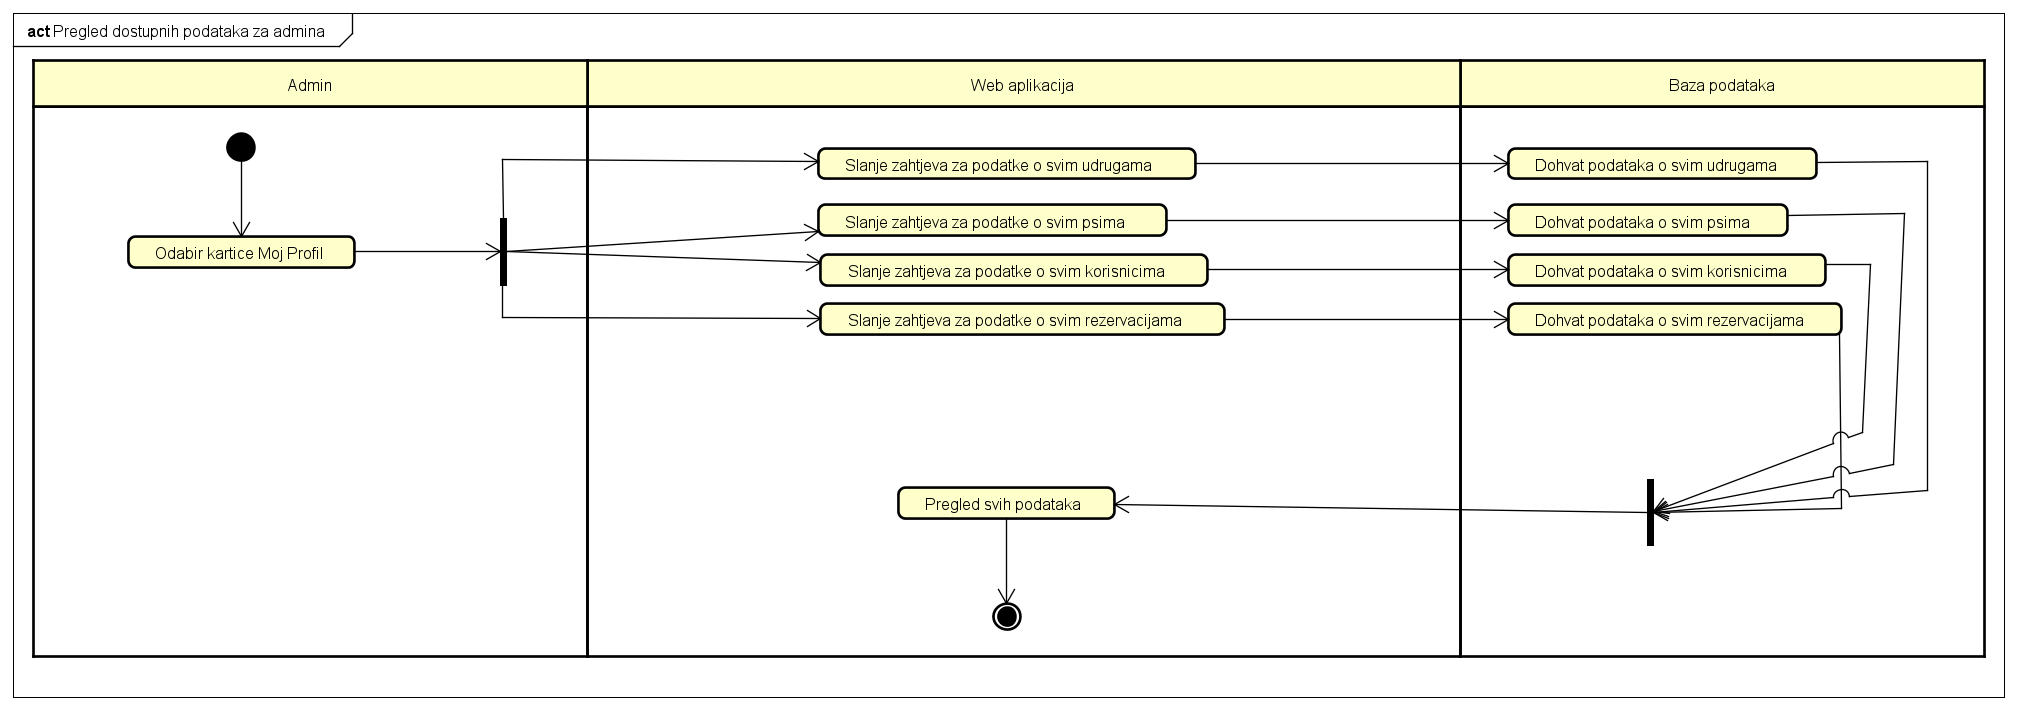
\includegraphics[scale=0.3]{dijagrami/Pregled_dostupnih_podataka_za_admina.png}
			\centering
			\caption{Dijagram aktivnosti za pregled dostupnih podataka za admina}
			\label{fig:activity_diagram_12}
		\end{figure}
			
			\eject
		\section{Dijagram komponenti}
		Dijagram komponenti je strukturni, statički UML dijagram koji vizualizira organizaciju i međuovisnost komponenata aplikacije, s naglaskom na implementaciju sustava, stoga je koristan za stjecanje okvirne ideje o implementaciji sustava, bez ulaženja u prevelike detalje.
		 
		U prikazanom dijagramu našu aplikaciju smo podijelili na 4 glavne komponente:komponentu React view, koji je zadužen za de-facto upravljanje cijelom aplikacijom, komponentu frontend logike, zaduženu za dohvat odgovarajućih HTML, CSS i .js datoteka, komponentu backend logike, zaduženu za dohvat i obradu podataka iz baze, te samu SQL bazu podataka.
		
		Preko sučelja za dohvat HTML-a, CSS-a i .js datoteka pristupa se komponenti frontend logike. Njen centralni dio je router komponenta (u našem slučaju datoteka App.js), zadužena za usklađivanje rada ostalih komponenti i određivanje koja će se datoteka proslijediti za prikaz u klijentovom browseru. Naravno, sve frontend komponente ovise o React biblioteci.
		
		Komunikacija s komponentom backend logike se odvija preko REST sučelja (zahtjevi GET, PUT, POST, DELETE). Zahtjevi se, nakon primitka u kontrolerima, prosljeđuju servisima, odnosno komponentama repozitorija, koji preko sučelja JpaRepository komunicira s bazom i dohvaća tražene podatke. Prijenos podataka između komponenti backend logike ostvaren je korištenjem DTO klasa, stoga sve komponente imaju ovisnost prema njima. Sve backend komponente ovise o Spring biblioteci (naravno, osim baze, no ona je zasebna komponenta u odnosu na backend).
		
		\begin{figure}[H]
			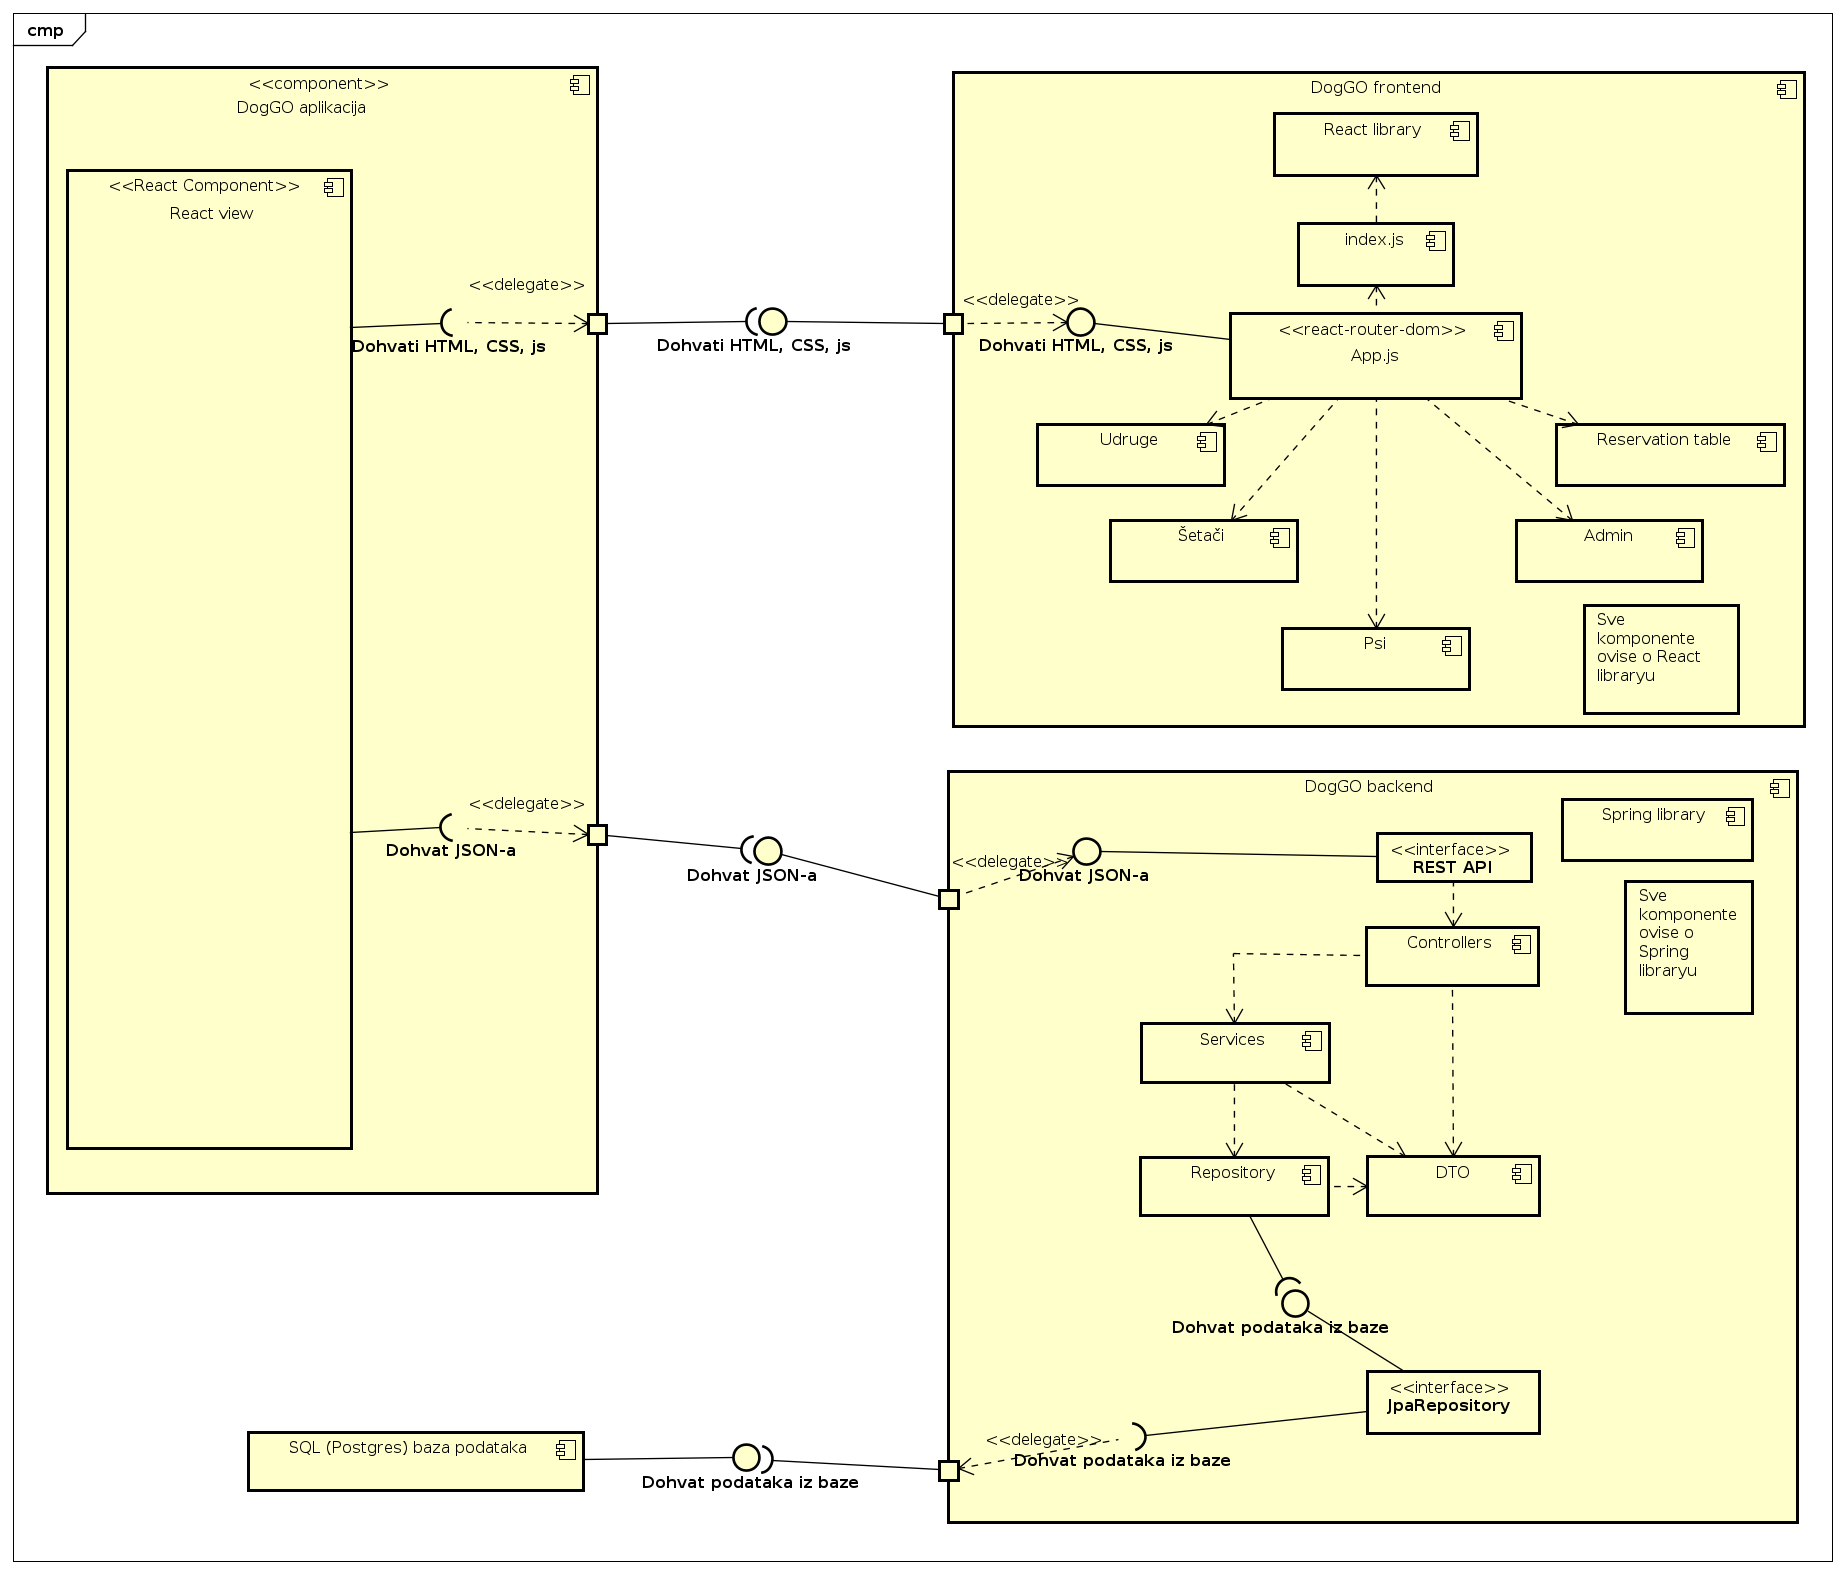
\includegraphics[scale=0.3]{dijagrami/component_diagram.png}
			\centering
			\caption{Dijagram komponenti}
			\label{fig:domain}
		\end{figure}
		
	\chapter{Implementacija i korisničko sučelje}
		
		
		\section{Korištene tehnologije i alati}
		
			\subsection{Backend tehnologije}
			
			Odabrani programski jezik \textit{backenda} naše web-aplikacije jest \uline{Java}\footnote{\url{https://www.java.com/en/}} u sklopu razvojnog okvira \uline{Spring Boot}\footnote{\url{https://spring.io/}} koji pruža razrađeni model programiranja i konfiguracije te je jedan od najčešće korištenih Java EE okvira za izgradnju aplikacija. Korištene su i pripadne \uline{Spring Data}\footnote{\url{https://spring.io/projects/spring-data}} i \uline{Spring Security}\footnote{\url{https://spring.io/projects/spring-security}} podrške. Za strukturiranje i automatizaciju razvojnog ciklusa projekta korišten je alat \uline{Maven}\footnote{\url{https://maven.apache.org/}}. Odabrani sustav upravljanja relacijskim bazama podataka jest \uline{PostgreSQL}\footnote{\url{https://www.postgresql.org/}}, dok je u razvojnoj i testnoj fazi projekta korišten \textit{in-memory} sustav \uline{H2}\footnote{\url{https://www.h2database.com/}}. Za lakšu navigaciju i testiranje aplikacijskog programskog sučelja  korišten je alat \uline{Swagger UI}\footnote{\url{https://swagger.io/tools/swagger-ui/}}. Za generiranje PDF dokumenata unutar aplikacije,  korištena je knjižica \uline{IText}\footnote{https://itextpdf.com/en}. Korištena razvojna okruženja na \textit{backendu} su \uline{Eclipse IDE}\footnote{\url{https://www.eclipse.org/eclipseide/}} i \uline{IntelliJ IDEA}\footnote{\url{https://www.jetbrains.com/idea/}}.
			
			\subsection{Frontend tehnologije}
			Korisničko sučelje aplikacije temeljeno je na označnom jeziku \uline{HTML5}\footnote{\url{https://html.spec.whatwg.org/}} i stilskom jeziku \uline{CSS}\footnote{\url{https://www.w3.org/Style/CSS/Overview.en.html}} . Modelirano je pomoću razvojnog okvira \uline{React}\footnote{\url{https://reactjs.org/}} u programskom jeziku \uline{JavaScript}. React se koristi za izradu jednostraničnih aplikacija, tj. stranica koje komuniciraju s korisnikom dinamički mijenjajući trenutnu web stranicu umjesto učitavanja cijele nove stranice. Složenije jednostranične aplikacije osim React-a koriste i niz drugih knjižica za nadogradnju komponenti. Za upravljanje knjižicama koristi se \uline{npm}\footnote{\url{https://www.npmjs.com/}}. Neke od mnogih korištenih knjižica u izrađenoj aplikaciji su \uline{Bootstrap}\footnote{\url{https://getbootstrap.com/}}, \uline{Material UI}\footnote{\url{https://material-ui.com/}}, \uline{Semantic UI}\footnote{\url{https://semantic-ui.com/}} i \uline{Redux}\footnote{https://redux.js.org/}. Korištena razvojna okolina na \textit{frontendu} jest \uline{Visual Studio Code}\footnote{\url{https://code.visualstudio.com/}}.
			
			 \subsection{Puštanje u pogon}
            Cijeli sustav uspostavljen je i pušten u pogon na platformi \uline{Heroku}\footnote{\url{https://www.heroku.com/}}, servisu temeljenom na oblaku.
            
			\subsection{Dokumentacija}
			Za dokumentaciju programskog riješenja korišten je \uline{Astah}\footnote{https://astah.net/}, alat za modeliranje UML dijagramima. Za vizualizaciju i modeliranje baze podataka korišten je alat \uline{Erdplus}\footnote{https://erdplus.com/}.
			
			\subsection{Timska komunikacija}
			Za svrhe komunikacije unutar tima korištene su sljedeće platforme: 
			\begin{itemize}
			    \itemsep-0.5em
			    \item  \uline{Trello}\footnote{\url{https://trello.com/en}} - organizacijska platforma temeljena na kanban metodi
			    \item \uline{Discord}\footnote{\url{https://discord.com/}} - VoIP platforma za brzu komunikaciju
			    \item \uline{WhatsApp}\footnote{\url{https://www.whatsapp.com/}} - aplikacija za razmjenu poruka
			    \item \uline{Microsoft Teams}\footnote{\url{https://www.microsoft.com/en-us/microsoft-365/microsoft-teams/group-chat-software}} -  platforma za video konferencije
			\end{itemize}
			\medskip
			\noindent Za distribuirano upravljanje kodom i verzioniranje korišten je sustav \uline{Git}\footnote{\url{https://git-scm.com/}} s udaljenim repozitorijem posluženim na \uline{GitLab}\footnote{\url{https://about.gitlab.com/}} platformi.
	        \eject 
		
	
		\section{Ispitivanje programskog rješenja}
			
			\subsection{Ispitivanje komponenti}
			
			Uspješna rezervacija je temeljna funkcionalnost ove aplikacije. JUnit testovima ispitani su rubni i redovni slučajevi te oni koji izazivaju pogreške. Priložen je kod kojim su u bazu dodani entiteti potrebni za ispitivanje funkcionalnosti rezervacije te kod Junit testova. 
			
			\begin{figure}[H]
				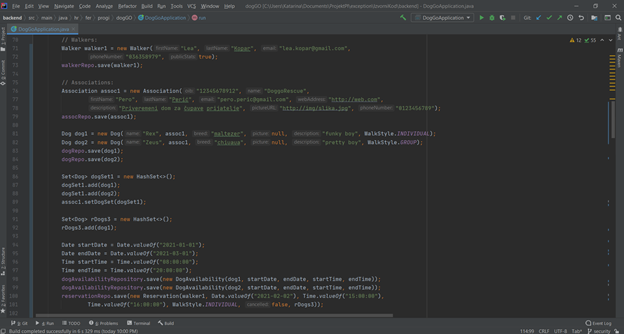
\includegraphics[scale=1]{slike/ispitivanje-sustava-1.png} 
				\centering
				\caption{Prikaz inicijalizacije testnih podataka}
				\label{fig:testiranje}
			\end{figure}
			
			\noindent \textbf{Ispitni slučaj 1: Pokušaj rezervacije gdje je sat početka vremenski nakon sata završetka šetnje}
			
			Nije moguće napraviti rezervaciju na isti dan, a da je pritom vrijeme početka šetnje veće od vremena završetka šetnje. Sljedećim testom izazivamo iznimku RequestDeniedException s odgovarajućom porukom
			
			\begin{figure}[H]
				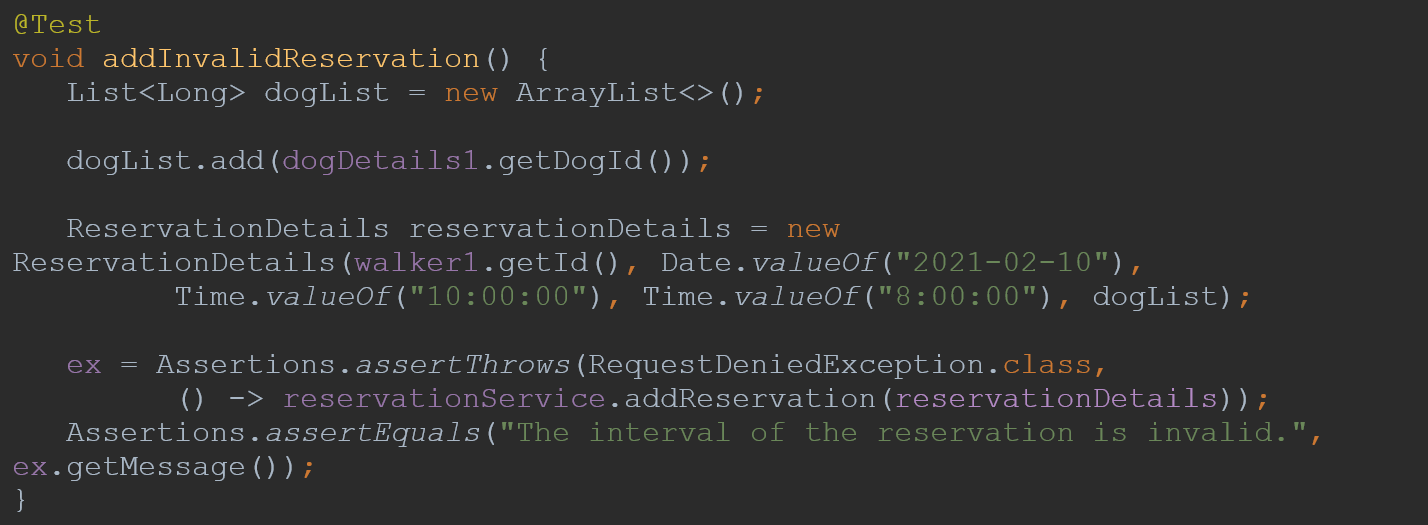
\includegraphics[scale=0.6]{slike/junit-1.PNG}
				\centering
				\caption{Prikaz 1. Junit testa}
				\label{fig:testiranje}
			\end{figure}
			
			\noindent \textbf{Ispitni slučaj 2: Pokušaj rezervacije gdje je pas za grupnu šetnju jedini u rezervaciji}
			
			Psi koji su namijenjeni grupnoj šetnji ne mogu biti jedini u rezervaciji, stoga sljedećim testom želimo napraviti rezervaciju s listom pasa koja ima samo jednog psa, a koji mora biti u grupi s još minimalno jednim psom da bi rezervacija bila uspješna. Pokušaj rezervacije završava iznimkom RequestDeniedException s odgovarajućom porukom.
			
			\begin{figure}[H]
				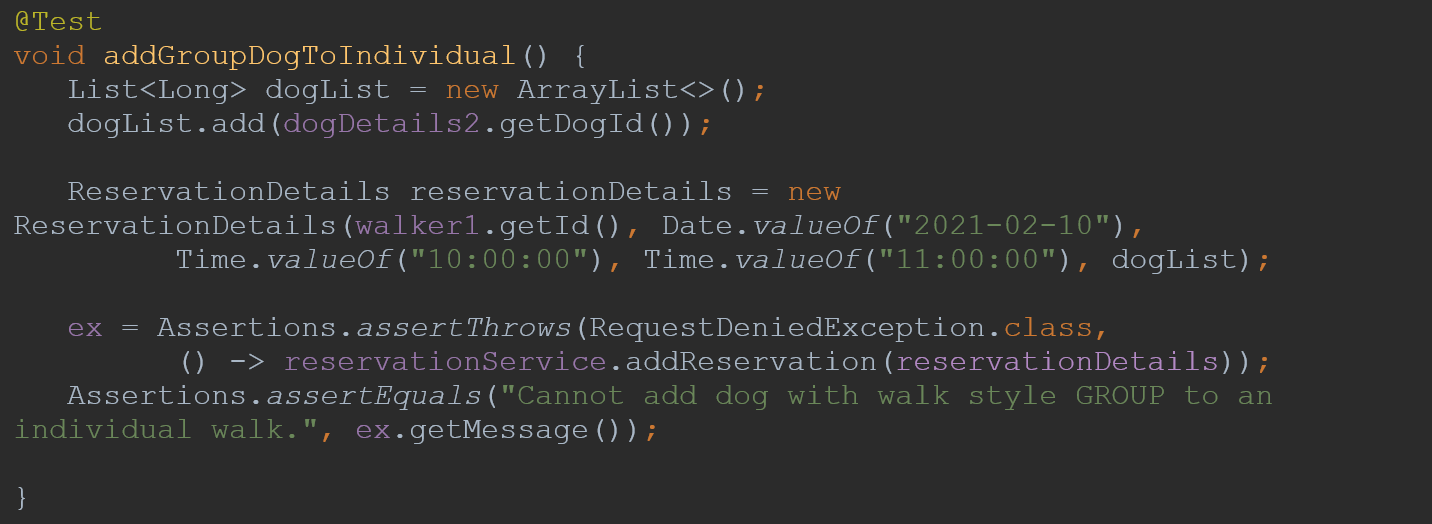
\includegraphics[scale=0.6]{slike/junit-2.PNG}
				\centering
				\caption{Prikaz 2. Junit testa}
				\label{fig:testiranje}
			\end{figure}
			
			\noindent \textbf{Ispitni slučaj 3: Pokušaj rezervacije gdje je pas za individualnu šetnju dodan u grupnu šetnju}
			
			Psi koji su namijenjeni individualnoj šetnji ne mogu biti stavljeni u grupnu šetnju, pa pokušaj rezervacije gdje je takav pas stavljen u grupu s drugima izaziva RequestDeniedException iznimku s odgovarajućom porukom.
			
			\begin{figure}[H]
				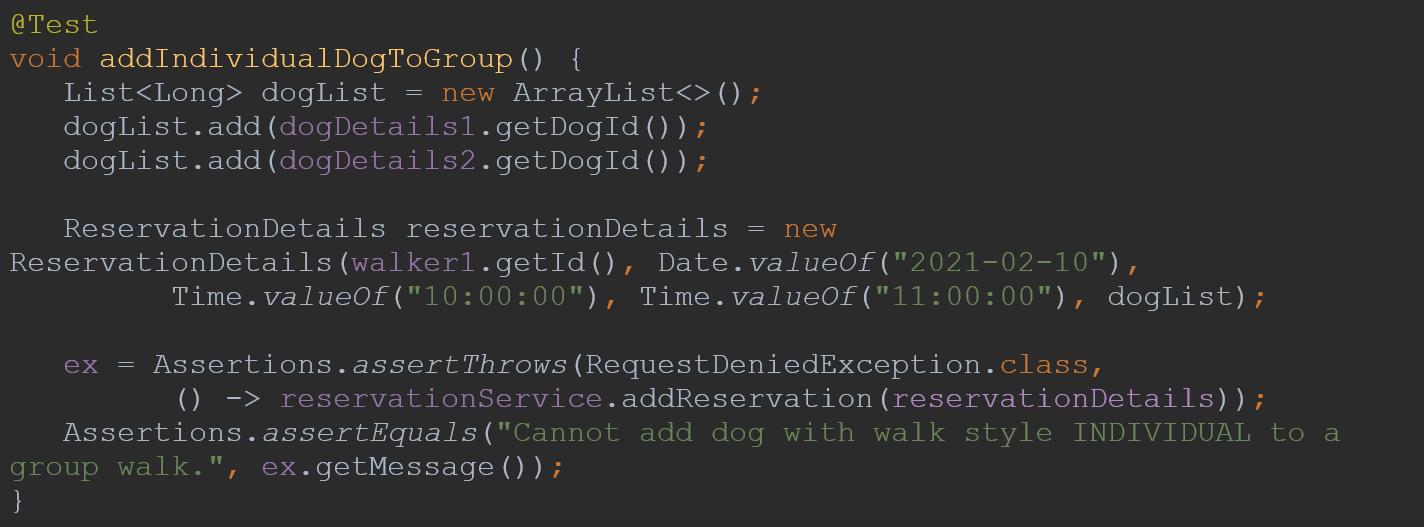
\includegraphics[scale=0.6]{slike/junit-3.PNG}
				\centering
				\caption{Prikaz 3. Junit testa}
				\label{fig:testiranje}
			\end{figure}
			
			\noindent \textbf{Ispitni slučaj 4: Pokušaj rezervacije kada je pas nedostupan}
			
			Ako se pokuša napraviti rezervacija u terminu kada pas nije dostupan, potrebno je izazvati iznimku RequestDeniedException s odgovarajućom porukom.
			
			\begin{figure}[H]
				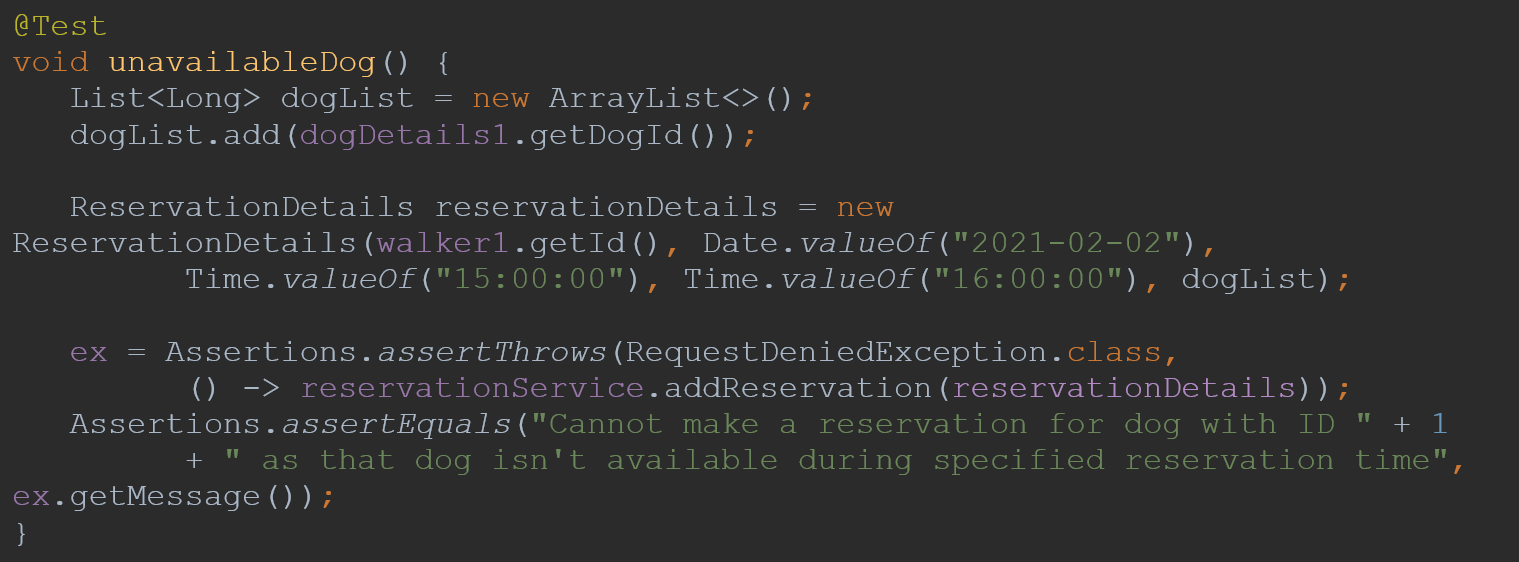
\includegraphics[scale=0.6]{slike/junit-4.PNG}
				\centering
				\caption{Prikaz 4. Junit testa}
				\label{fig:testiranje}
			\end{figure}
			
			\noindent \textbf{Ispitni slučaj 5: Pokušaj rezervacije kada je šetač nedostupan}
			
    		Ako šetač pokuša napraviti rezervaciju u terminu u kojem je već prije napravio rezervaciju također se izaziva RequestDeniedException s odgovarajućom porukom. 
			
			\begin{figure}[H]
				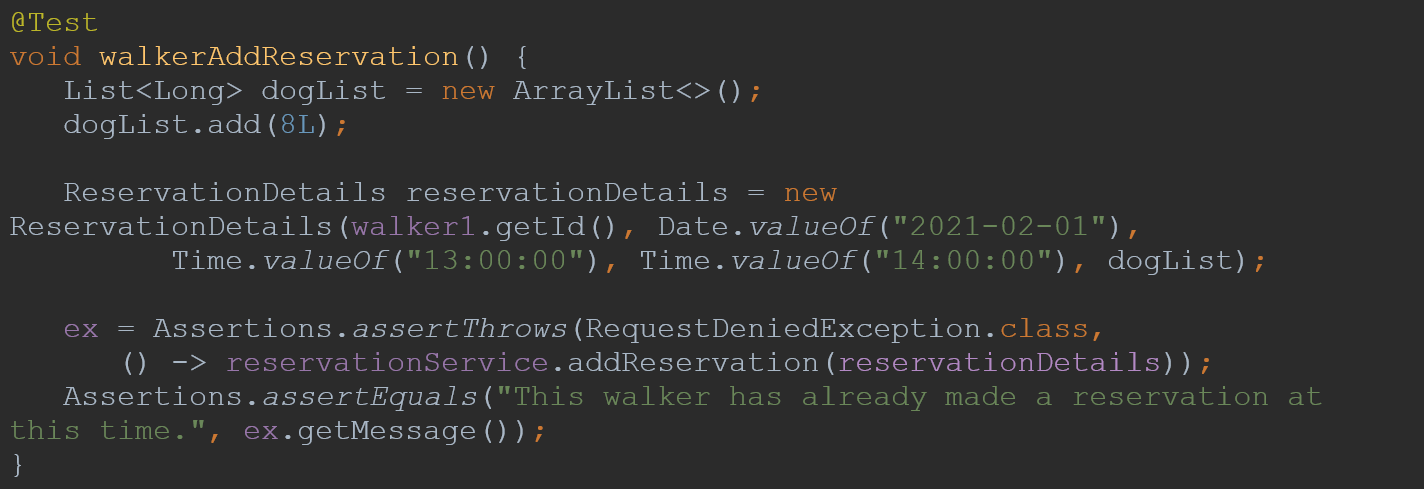
\includegraphics[scale=0.6]{slike/junit-5.PNG}
				\centering
				\caption{Prikaz 5. Junit testa}
				\label{fig:testiranje}
			\end{figure}
			
			\noindent \textbf{Ispitni slučaj 6: Pokušaj rezervacije kada je šetač nedostupan}
			
    		Najbitnije je ispitati je li rezervacija koja ispunjava sve uvjete uspješno napravljena. Sljedećim testom provjeravamo jednakost hardkodiranih detalja rezervacije i detalja metode kojom vraćaju detalji uspješne rezervacije.
			
			\begin{figure}[H]
				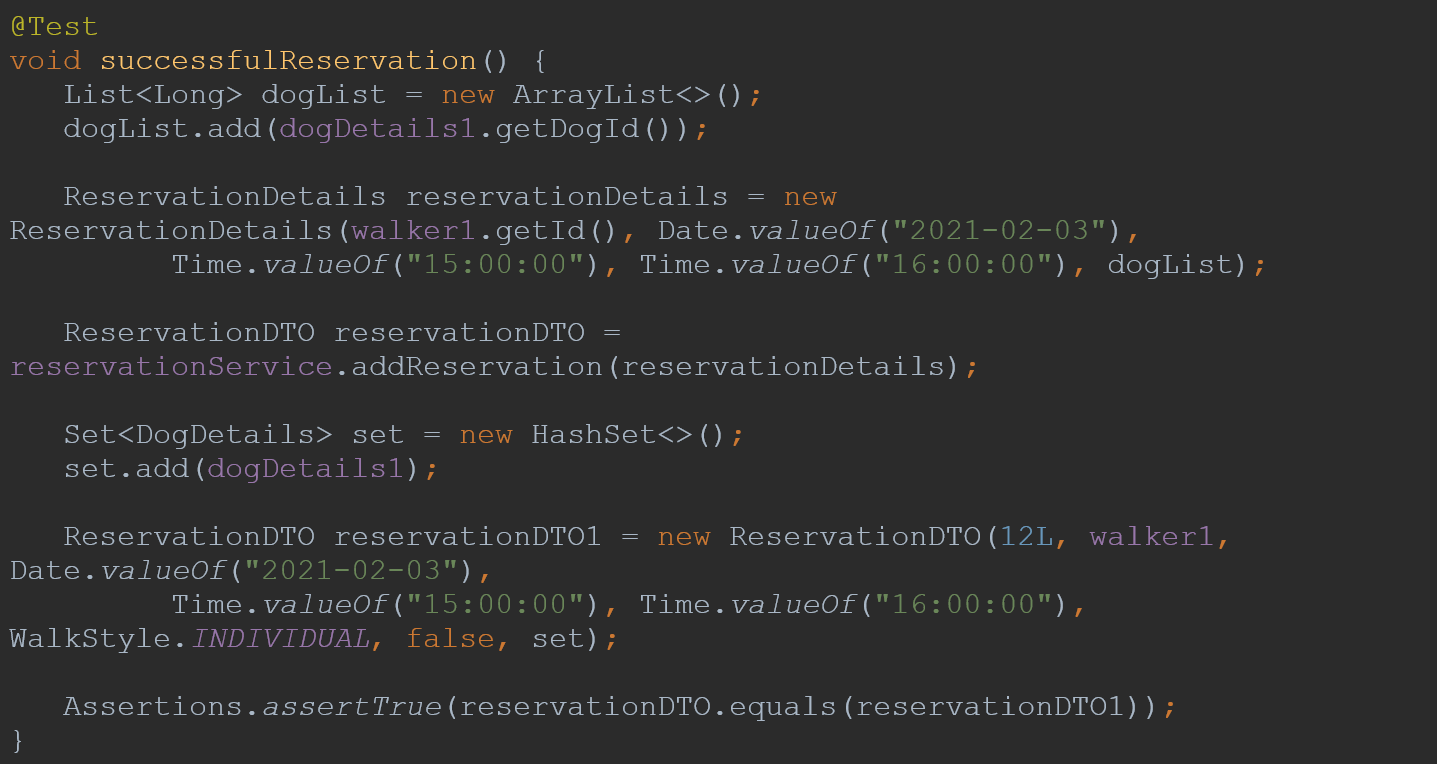
\includegraphics[scale=0.6]{slike/junit-6.PNG}
				\centering
				\caption{Prikaz 6. Junit testa}
				\label{fig:testiranje}
			\end{figure}
			
			\noindent \textbf{Rezultati testiranja}
			
			Svi navedeni Junit testovi su se uspješno proveli.
			
			\begin{figure}[H]
				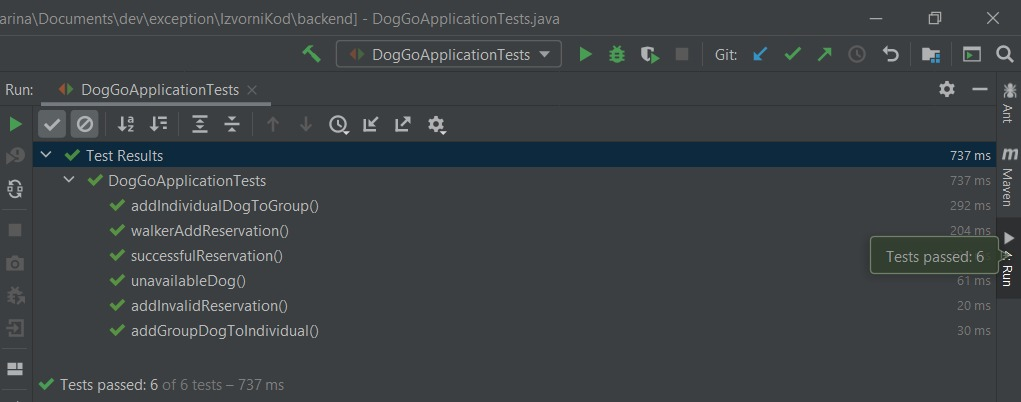
\includegraphics[scale=0.4]{slike/tests-passed.JPEG}
				\centering
				\caption{Prikaz rezultata testova}
				\label{fig:testiranje}
			\end{figure}
			
			\subsection{Ispitivanje sustava}
			
			\noindent \textbf{Ispitni slučaj 1: Rezervacija šetnje}
			
			\noindent \textbf{Ulaz:}
			\begin{packed_enum}
				
				\item Otvaranje početne stranice u web pregledniku.
				\item Otvaranje stranice popisa udruge.
				\item Odabir udruge i pritisak kursorom na gumb REZERVIRAJ.
				\item Odabir datuma i vremenskog intervala šetnje.
				\item Pritisak kursorom na gumb Rezerviraj.
				
			\end{packed_enum}
			\textbf{Očekivani rezultat:}
			\begin{packed_enum}
				
				\item Prikaz naslovne stranice.
				\item Prikaz popisa udruge.
				\item Prikaz profila udruge i popis pasa.
				\item Prikaz forme za rezervaciju i prikaz odabranog datuma i vremenskih intervala šetnje.
				\item Prikaz poruke uspješne rezervacije i profila udruge.
				
			\end{packed_enum}
			\textbf{Rezultat:} Očekivani rezultat [4.] nije zadovoljen jer je isteklo implicitno vrijeme čekanja. Zbog toga se očekivani rezultat [5.] nije odradio. \textcolor{red}{Aplikacija nije prošla test.}
			
			\begin{figure}[H]
				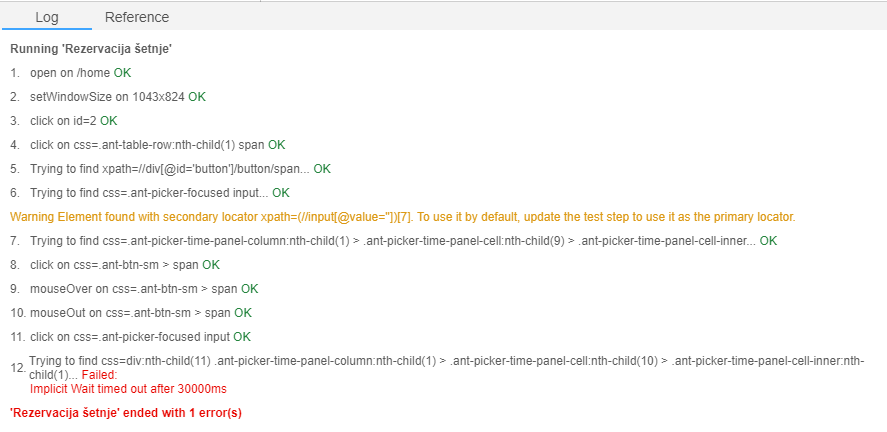
\includegraphics[scale=0.6]{slike/rezervacijaSetnje.PNG} 
				\centering
				\caption{Prikaz rezultata 1. ispitnog slučaja u Selenium-u}
				\label{fig:sustav-prvi-slucaj}
			\end{figure}
		
			\noindent \textbf{Ispitni slučaj 2: Otkazivanje šetnje od strane udruge}
			
			\noindent \textbf{Ulaz:}
			\begin{packed_enum}
				
				\item Otvaranje početne stranice u web pregledniku.
				\item Otvaranje profila udruge.
				\item Odabir popisa rezervacija udruge.
				\item Pritisak kursorom na gumb OTKAŽI.
				
			\end{packed_enum}
			\textbf{Očekivani rezultat:}
			\begin{packed_enum}
				
				\item Prikaz naslovne stranice.
				\item Prikaz profila udruge i popis pasa.
				\item Prikaz popisa rezervacija na profilu udruge.
				\item Prikaz profila udruge i popis pasa.
				
			\end{packed_enum}
			\textbf{Rezultat:} \textcolor{red}{Aplikacija je prošla test.}
			
			\begin{figure}[H]
				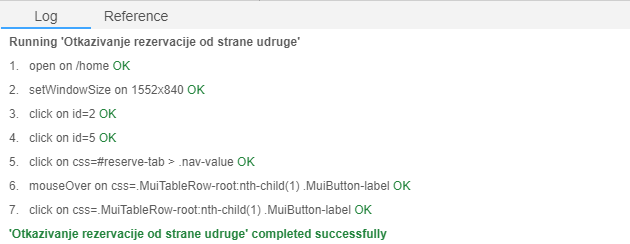
\includegraphics[scale=0.7]{slike/otkazivanjeRezervacijeOdStraneUdruge.PNG} 
				\centering
				\caption{Prikaz rezultata 2. ispitnog slučaja u Selenium-u}
				\label{fig:sustav-drugi-slucaj}
			\end{figure}
		
			\noindent \textbf{Ispitni slučaj 3: Otkazivanje šetnje od strane admina}
			
			\noindent \textbf{Ulaz:}
			\begin{packed_enum}
				
				\item Otvaranje početne stranice u web pregledniku.
				\item Otvaranje admin profila.
				\item Pomicanje ekrana do prikaza popisa rezervacija.
				\item Pritisak kursorom na gumb OTKAŽI.
				
			\end{packed_enum}
			\textbf{Očekivani rezultat:}
			\begin{packed_enum}
				
				\item Prikaz naslovne stranice.
				\item Prikaz admin profila.
				\item Prikaz popisa rezervacija na admin profilu.
				\item Prikaz ažuriranog popisa rezervacija na admin profilu.
				
			\end{packed_enum}
			\textbf{Rezultat:} \textcolor{red}{Aplikacija je prošla test.}
			
			\begin{figure}[H]
				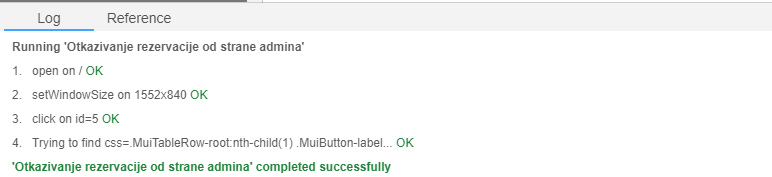
\includegraphics[scale=0.7]{slike/otkazivanjeRezervacijeOdStraneAdmina.PNG} 
				\centering
				\caption{Prikaz rezultata 3. ispitnog slučaja u Selenium-u}
				\label{fig:sustav-treci-slucaj}
			\end{figure}
			\eject 
		
		
		\section{Dijagram razmještaja}
			
			 Dijagram razmještaja opisuje topologiju sustava i usredotočen je na odnos sklopovskih i programskih dijelova. 
			 Arhitektura sustava DogGO aplikacije je ”klijent – poslužitelj” gdje web poslužitelj i poslužitelj baze podataka se nalaze na poslužiteljskom računalu a klijenti koriste web preglednik kako bi pristupili web aplikaciji. Komunikacija između računala korisnika i poslužitelja odvija se preko HTTP veze.
			 
			 \begin{figure}[H]
				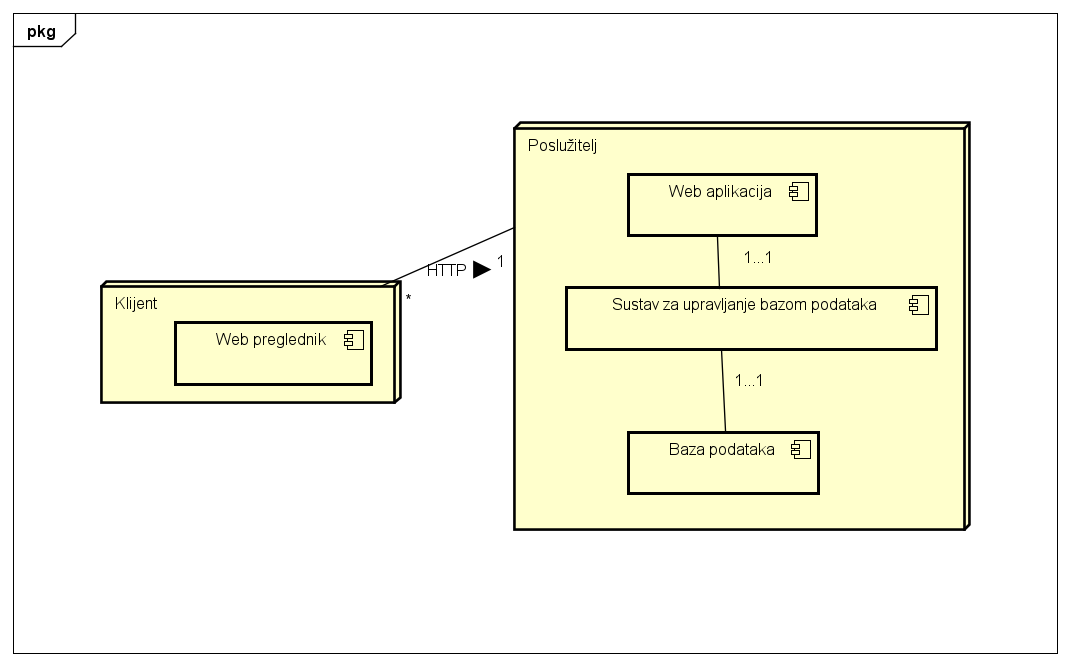
\includegraphics[scale=0.6]{dijagrami/deploy.png} 
				\centering
				\caption{Dijagram razmještaja}
				\label{fig:dijagram-razmjestaja}
			\end{figure}
			
			\eject 
		
		\section{Upute za puštanje u pogon}
			
			Puštanje aplikacije u pogon možemo podijeliti na 3 glavna koraka
			         \begin{packed_item}
                            \item[$\bullet$] pokretanje Postgres baze
                            \item[$\bullet$] pokretanje backenda (Spring Boot)
                            \item[$\bullet$] pokretanje frontenda (npm, React)
                    \end{packed_item}
                    
                \subsection{Pokretanje baze}
                
                Za pokretanje baze prvo je potrebno skinuti Postgres bazu. Preuzmemo installer sa \textit{https://www.postgresql.org/download/} (verzija 13), te slijedimo upute za instalaciju. Zatim preuzimamo i instaliramo PgAdmin (\textit{https://www.pgadmin.org/download/}), koji nam olakšava upravljanje bazom i pregled podataka. \newline
                
                \noindent Nakon instalacije navedenih komponenti, moramo još kreirati bazu, odnosno korisničko ime koje ćemo koristiti za spajanje na bazu.\newline
                
                \noindent 1) Otvorimo pgAdmin. Prilikom prvog pokretanja, aplikacija nas traži upisivanje glavne lozinke, koji smislimo i upišemo. Zatim klikom na Login/Group Roles -> Create otvaramo izbornik za stvaranje novog korisnika.
                
                    \begin{figure}[H]
        				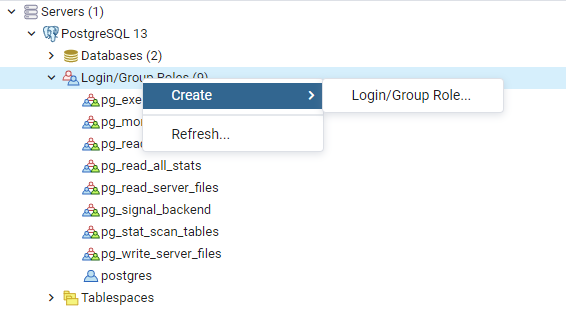
\includegraphics[scale=0.6]{slike/deploy_kreiranje_usera1.PNG} 
        				\centering
        				\caption{Kreiranje usera}
        				\label{fig:sustav-prvi-slucaj}
        			\end{figure}
        			
        		U odgovarajuća polja upišemo željeno korisničko ime i password (u primjeru korišten exampleUser/password123)
                
                    \begin{figure}[H]
        				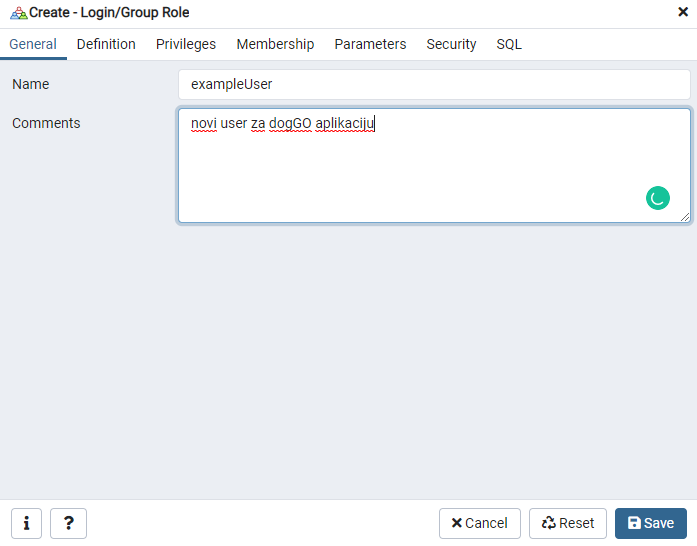
\includegraphics[scale=0.6]{slike/deploy_kreiranje_usera2.PNG} 
        				\centering
        				\caption{Kreiranje usera - upis korisničkog imena}
        				\label{fig:sustav-prvi-slucaj}
        			\end{figure}
        			
        			 \begin{figure}[H]
        				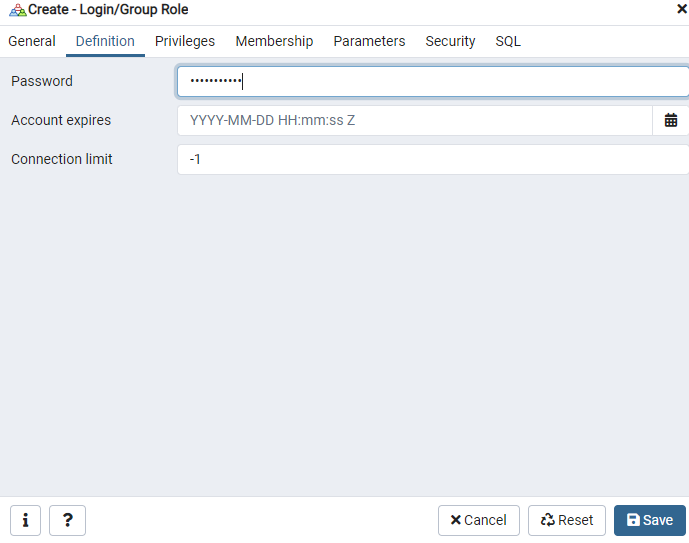
\includegraphics[scale=0.6]{slike/deploy_kreiranje_usera3.PNG} 
        				\centering
        				\caption{Kreiranje usera 3 - upis lozinke}
        				\label{fig:sustav-prvi-slucaj}
        			\end{figure}
                
                Nakon što smo stvorili korisnika, možemo stvoriti i novu bazu.
                
                    \begin{figure}[H]
        				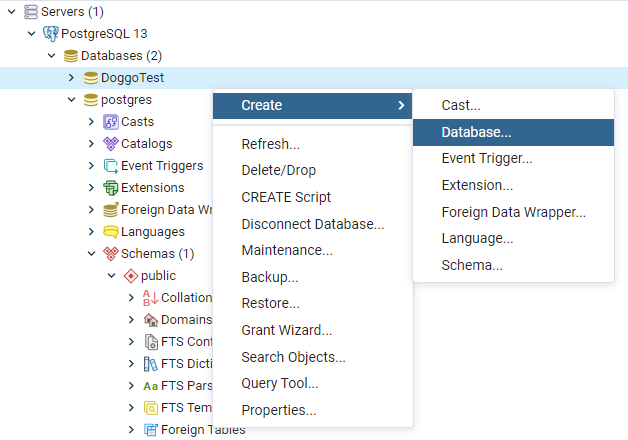
\includegraphics[scale=0.6]{slike/deploy_kreiranje_baze1.PNG} 
        				\centering
        				\caption{Izbornik za stvaranje baze}
        				\label{fig:sustav-prvi-slucaj}
        			\end{figure}
        			
        			Jedino što je potrebno upisati je ime baze (u primjeru DoggoExample), te vlasnika baze - novostvoreni korisnik exampleUser.
        			
        			 \begin{figure}[H]
        				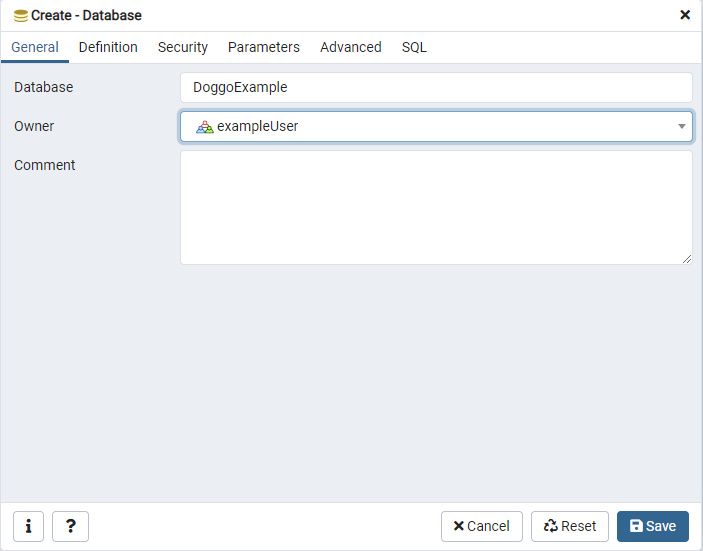
\includegraphics[scale=0.6]{slike/deploy_kreiranje_baze2.PNG} 
        				\centering
        				\caption{Izbornik za stvaranje baze - upis imena i vlasnika}
        				\label{fig:sustav-prvi-slucaj}
        			\end{figure}
        			
        			
                
                \subsection{Pokretanje backenda}
                
                Za ispravno pokretanje backenda, prvo moramo instalirati sljedeće aplikacije
			         \begin{packed_item}
                            \item[$\bullet$] alat za upravljanje kodom Maven (najnovija trenutačna verzija). Ukoliko se backend pokreće iz naredbenog retka sa naredbom mvnw, instalacija nije potrebna (tj. mvnw je maven wrapper, program koji sam preuzima i privremeno instalira potrebnu verziju Mavena)
                            \begin{packed_item}
                                \item[$\bullet$] za instalaciju slijedimo upute na \textit{https://maven.apache.org/install.html}
                            \end{packed_item}
                            \item[$\bullet$] Java verzije 15 ili novija
                            \begin{packed_item}
                                \item[$\bullet$] za instalaciju slijedimo upute na \textit{https://docs.oracle.com/en/java/javase/15/install/overview-jdk-installation.html}
                            \end{packed_item}
                            \item[$\bullet$] (opcionalno) neki IDE (IntelliJ/Eclipse)
                    \end{packed_item}
                    
                    \noindent Nakon preuzimanja svih potrebnih aplikacija, prvo moramo podesiti spajanje na našu novostvorenu bazu. U nekom uređivaču teksta ili IDE-u otvorimo datoteku IzvorniKod/backend/src/main/java/resources/application.properties, te tamo unesemo sljedeće podatke:
                    
                    \begin{figure}[H]
        				\includegraphics[scale=0.6]{slike/deploy_applicationproperties.PNG} 
        				\centering
        				\caption{application.properties}
        				\label{fig:sustav-prvi-slucaj}
        			\end{figure}
                    
                    U ovom trenutku imamo sve spremno za pokretanje backenda, što možemo učiniti na 2 načina:\newline \\
                    
                    \noindent a) Korištenjem naredbenog retka (command line)
                    Za pokretanje iz naredbenog retka korištenjem Windows powershella/Linux terminala ili slično pozicioniramo se u direktorij IzvorniKod/backend/
                    te tamo pokrenemo naredbu \textbf{mvn clean install}. Nakon dovršenja ove naredbe, iz istog direktorija pokrenemo i \textbf{mvn spring-boot:run}. Aplikacija se pokrenula na URL-u http://localhost:8080.\newline

                    \noindent b) Korištenjem IDE-a (IntelliJ)
                    Za pokretanje aplikacije iz IDE-a, prvo moramo otvoriti naš projekt u IntelliJ-u. 
                    Klikom na File/Open otvara nam se izbornik u kojem pronađemo naš projekt te u njemu odaberemo folder backend.
                    
                    \begin{figure}[H]
        				\includegraphics[scale=0.6]{slike/deploy_ideizbornik.PNG} 
        				\centering
        				\caption{Otvaranje projekta u IntelliJ-u}
        				\label{fig:sustav-prvi-slucaj}
        			\end{figure}
        			
        			Nakon otvaranja projekta, u gornjem desnog uglu pronađemo zelenu ikonicu u obliku trokuta, te ju kliknemo. Klikom na nju, aplikacija se pokreće na URL-u http://localhost:8080.
        			
        			 \begin{figure}[H]
        				\includegraphics[scale=1]{slike/deploy_runappide.PNG} 
        				\centering
        				\caption{Pokretanje aplikacije iz IntelliJ-a}
        				\label{fig:sustav-prvi-slucaj}
        			\end{figure}
        			
                \subsection{Pokretanje frontenda}
                
                Za pokretanje iz naredbenog retka potrebno se pozicionirati u direktorij IzvorniKod/frontend/app/src i u njemu izvesti sljedeće naredbe:

                \textbf{npm install}
                
                \noindent Naredba instalira sve node module potrebne za pokretanje aplikacije.\newline
                
                \textbf{npm start}
                
                \noindent Pokreće aplikaciju na http://localhost:3000.
                Stranica se ponovno učitava svakom spremljenom promjenom u kodu.

			
			
			\eject 
	\chapter{Zaključak i budući rad}

Primarni cilj ovog projekta bio je razviti aplikaciju koja omogućuje građanima da ugovore šetnje pasa u skloništima za pse i tako pomognu u socijalizaciji pasa i povećaju vjerojatnost udomljavanja. Iz projektnog zadatka bilo je potrebno izlučiti funkcionalne i nefunkcionalne zahtjeve, konceptualno osmisliti i dokumentirati aplikaciju a zatim provesti implementaciju osmišljenog.
		
Provedba projekta bila je podijeljena u dva ciklusa. U prvom ciklusu oformili smo projektni tim, uspostavili kanale komunikacije i započeli s radom. Bilo nam je važno upoznati se i pokušati stvoriti dobru radnu atmosferu, usprkos tome što je komunikacija uživo bila otežana. Za brzu komunikaciju smo odabrali WhatsApp, a organizaciju projekta radili smo na stranici Trello koja podržava kanban metodu organizacije. Vrlo intenzivnim fokusom na razradu zahtjeva odmah na početku rada, stvorili smo čvrstu bazu za daljnji rad i osigurali da je svim članovima tima jasna slika aplikacije koju izrađujemo. 
		
U drugom ciklusu veći naglasak bio je na samoj implementaciji aplikacije. S obzirom na to da su svim članovima tima tehnologije s kojima smo radili bile dosad nepoznate, u drugom ciklusu se pokazala posvećenost i inicijativa članova. Svi članovi su samostalno istraživali tehnologije i tražili rješenja za probleme koji su se pojavljivali. Također je do izražaja došla važnost komunikacije i surađivanja. Nakon nekoliko nesporazuma i udvostručavanja odrađenog posla, stavili smo veći naglasak na poboljšanje komunikacije i učestalo izvještavanje o problemima koje treba riješiti za napredak. Počeli smo koristiti Discord koji nam je omogućio da više timova radi istovremeno na različitim komponentama i međusobno se brzo posavjetuje.
		
Radom na projektu svi smo stekli nova znanja i zato bismo da sada krećemo s projektom neke probleme vjerojatno riješili na brži i kvalitetniji način. U budućoj nadogradnji aplikacije vjerojatno bi započeli s refaktoriranjem pojedinih dijelova koda koji su nekonzistentni ili smo iskustvom rada na drugim komponentama uvidjeli da se mogu bolje riješiti. Osim toga, kao moguće proširenje funkcionalnosti aplikacije dodali bismo mogućnost grupnih šetnja s drugim ljudima, što mislimo da bi bilo zanimljivo i za prijatelje i za upoznavanje novih ljudi.

Svim članovima tima je ovaj projekt pružio nova znanja i vještine s kojima se dosad nismo susreli na FER-u. Osim tehničkih znanja iz korištenih tehnologija, stekli smo vrijedno iskustvo timskog rada i općenito samostalnog rada na projektu.
		
		\eject
	\chapter*{Popis literature}
		\addcontentsline{toc}{chapter}{Popis literature}
		
		\begin{enumerate}
			
			
			\item  Programsko inženjerstvo, FER ZEMRIS, \url{http://www.fer.hr/predmet/proinz}
			
			\item  I. Sommerville, "Software engineering", 8th ed, Addison Wesley, 2007.
			
			\item  T.C.Lethbridge, R.Langaniere, "Object-Oriented Software Engineering", 2nd ed. McGraw-Hill, 2005.
			
			\item  I. Marsic, "Software engineering book", Department of Electrical and Computer Engineering, Rutgers University, \url{http://www.ece.rutgers.edu/~marsic/books/SE}
			
			\item  The Unified Modeling Language, \url{https://www.uml-diagrams.org/}
			
			\item  Astah Community, \url{http://astah.net/editions/uml-new}
			
			\item L. Shklar, R. Rosen, "Web Application Architecture: Principles, Protocols, And Practices", 1st ed, John Wiley \& Sons Ltd, 2003.
			
			\item Službena dokumentacija Spring razvojnog okvira, \url{https://docs.spring.io/spring-framework/docs/current/reference/html/}
			
			\item Spring Boot backend demo aplikacija, CROZ d.o.o., \\ \url{https://gitlab.com/hrvojesimic/progi-project-teams-backend}
			
			\item Izrada frontenda u Reactu, CROZ d.o.o., \\
			\url{https://gitlab.com/jtomic/opp-project-teams-frontend/-/blob/master/education.md}
			
			\item Online platforma Baeldung, \url{https://www.baeldung.com/}
			
			\item Online platforma Spring.io, \url{https://spring.io/}
			
		\end{enumerate}
		
		 
	
	
	\begingroup
	\renewcommand*\listfigurename{Indeks slika i dijagrama}
	%\renewcommand*\listtablename{Indeks tablica}
	%\let\clearpage\relax
	\listoffigures
	%\vspace{10mm}
	%\listoftables
	\endgroup
	\addcontentsline{toc}{chapter}{Indeks slika i dijagrama}


	
	\eject 
		
	\chapter*{Dodatak: Prikaz aktivnosti grupe}
\addcontentsline{toc}{chapter}{Dodatak: Prikaz aktivnosti grupe}

\section*{Dnevnik sastajanja}

\begin{packed_enum}
	
	\item  sastanak
	\item[] \begin{packed_item}
		\item Datum: 8. listopada 2020.
		\item Prisustvovali: A.Terović, A.Miletić, D.Smoljan, E.Jagodić, F.Sentinella-Jerbić, I.Pezo, K.Golub
		\item Teme sastanka:
		\begin{packed_item}
			\item upoznavanje
			\item određivanje kanala komunikacije
			\item odabir teme
			\item odabir tehnologija
		\end{packed_item}
	\end{packed_item}
	
	\item  sastanak
	\item[] \begin{packed_item}
		\item Datum: 15. listopada 2020.
		\item Prisustvovali: A.Terović, A.Miletić, D.Smoljan, E.Jagodić, F.Sentinella-Jerbić, I.Pezo, K.Golub
		\item Teme sastanka:
		\begin{packed_item}
			\item definiranje funkcionalnosti
			\item raspodjela za pisanje dokumentacije
			\item tim za uspostavu baze podataka
			\item naziv aplikacije
		\end{packed_item}
	\end{packed_item}
	
	\item  sastanak
	\item[] \begin{packed_item}
		\item Datum: 22. listopada 2020.
		\item Prisustvovali: A.Terović, A.Miletić, D.Smoljan, E.Jagodić, F.Sentinella-Jerbić, I.Pezo, K.Golub
		\item Teme sastanka:
		\begin{packed_item}
			\item dodatne razrade funkcionalnosti
			\item podjela u timove za backend i frontend
			\item raspored stranica
		\end{packed_item}
	\end{packed_item}
	
	\item  sastanak
	\item[] \begin{packed_item}
		\item Datum: 3. studeni 2020.
		\item Prisustvovali: A.Terović, A.Miletić, D.Smoljan, E.Jagodić, F.Sentinella-Jerbić, I.Pezo, K.Golub
		\item Teme sastanka:
		\begin{packed_item}
			\item predstavljanje obavljenog na frontendu i backendu i dogovor oko nastavka rada
			\item podjela posljednjih zadataka prije prve predaje
			\item razmjena informacija o tehnologijama
		\end{packed_item}
	\end{packed_item}
	
	\item  sastanak
	\item[] \begin{packed_item}
		\item Datum: 10. studeni 2020.
		\item Prisustvovali: A.Terović, A.Miletić, D.Smoljan, E.Jagodić, F.Sentinella-Jerbić, I.Pezo, K.Golub
		\item Teme sastanka:
		\begin{packed_item}
			\item predstavljanje obavljenog na frontendu i backendu
			\item dogovaranje oko posljednjih promjena prije prve predaje
		\end{packed_item}
	\end{packed_item}
	
	\item  sastanak
	\item[] \begin{packed_item}
		\item Datum: 29. studeni 2020.
		\item Prisustvovali: A.Terović, A.Miletić, D.Smoljan, E.Jagodić, F.Sentinella-Jerbić, I.Pezo, K.Golub
		\item Teme sastanka:
		\begin{packed_item}
			\item prolazak kroz logiku aplikacije i priprema za kolokviranje prvog ciklusa
			\item bilježenje stvari koje treba popraviti u nastavku rada
		\end{packed_item}
	\end{packed_item}
	
	\item  sastanak
	\item[] \begin{packed_item}
		\item Datum: 7. prosinac 2020.
		\item Prisustvovali: A.Terović, A.Miletić, D.Smoljan, E.Jagodić, F.Sentinella-Jerbić, I.Pezo, K.Golub
		\item Teme sastanka:
		\begin{packed_item}
			\item bilježenje posla za drugi ciklus
			\item dodatna razrada nekih funkcionalnosti
			\item okvirna podjela posla
		\end{packed_item}
	\end{packed_item}
	
	\item  sastanak
	\item[] \begin{packed_item}
		\item Datum: 28. prosinac 2020.
		\item Prisustvovali: A.Terović, A.Miletić, D.Smoljan, E.Jagodić, F.Sentinella-Jerbić, I.Pezo, K.Golub
		\item Teme sastanka:
		\begin{packed_item}
			\item predstavljanje napravljenog
			\item rješavanje nejasnoća
			\item dodatna podjela posla za nastavak rada
		\end{packed_item}
	\end{packed_item}
	
	\item  sastanak
	\item[] \begin{packed_item}
		\item Datum: 5. siječnja 2021.
		\item Prisustvovali: A.Terović, A.Miletić, D.Smoljan, E.Jagodić, F.Sentinella-Jerbić, I.Pezo, K.Golub
		\item Teme sastanka:
		\begin{packed_item}
			\item rasprava o napravljenom
			\item potres usred sastanka
			\item završna podjela posla
		\end{packed_item}
	\end{packed_item}
	
	%
	
\end{packed_enum}

\eject
\section*{Tablica aktivnosti}



\begin{longtabu} to \textwidth {|X[7, l]|X[1, c]|X[1, c]|X[1, c]|X[1, c]|X[1, c]|X[1, c]|X[1, c]|}
	
	\cline{2-8} \multicolumn{1}{c|}{\textbf{}} &     \multicolumn{1}{c|}{\rotatebox{90}{\textbf{Eva Jagodić }}} & \multicolumn{1}{c|}{\rotatebox{90}{\textbf{Ana Terović }}} &	\multicolumn{1}{c|}{\rotatebox{90}{\textbf{Antonio Miletić }}} &	\multicolumn{1}{c|}{\rotatebox{90}{\textbf{Dorian Smoljan }}} &	\multicolumn{1}{c|}{\rotatebox{90}{\textbf{Fani Sentinella-Jerbić }}} &	\multicolumn{1}{c|}{\rotatebox{90}{\textbf{Iva Pezo }}} &	\multicolumn{1}{c|}{\rotatebox{90}{\textbf{Katarina Golub }}} \\ \hline 
	\endfirsthead
	
	
	\cline{2-8} \multicolumn{1}{c|}{\textbf{}} &     \multicolumn{1}{c|}{\rotatebox{90}{\textbf{Eva Jagodić }}} & \multicolumn{1}{c|}{\rotatebox{90}{\textbf{Ana Terović }}} &	\multicolumn{1}{c|}{\rotatebox{90}{\textbf{Antonio Miletić }}} &	\multicolumn{1}{c|}{\rotatebox{90}{\textbf{Dorian Smoljan }}} &	\multicolumn{1}{c|}{\rotatebox{90}{\textbf{Fani Sentinella-Jerbić }}} &	\multicolumn{1}{c|}{\rotatebox{90}{\textbf{Iva Pezo }}} &	\multicolumn{1}{c|}{\rotatebox{90}{\textbf{Katarina Golub }}} \\ \hline 
	\endhead
	
	
	\endfoot
	
	
	\endlastfoot
	
	Upravljanje projektom 		& 24 &  &  &  &  &  & \\ \hline
	Opis projektnog zadatka 	& 2 &  &  & 5 & 2 &  & \\ \hline
	
	Funkcionalni zahtjevi       &  &  &  &  & 5 & 4 &  \\ \hline
	Opis pojedinih obrazaca 	&  &  &  &  & 3 & 3 &  \\ \hline
	Dijagram obrazaca 			& 4 & 2 &  &  &  &  &  \\ \hline
	Sekvencijski dijagrami 		&  &  & 4 &  &  &  & 2 \\ \hline
	Opis ostalih zahtjeva 		&  &  &  &  & 1 &  &  \\ \hline
	
	Arhitektura i dizajn sustava	 &  &  &  &  & 9 &  &  \\ \hline
	Baza podataka				& 2 & 3 & 20 &  & 1 &  & 4  \\ \hline
	Dijagram razreda 			&  &  &  &  & 24 &  & 4  \\ \hline
	Dijagram stanja				&  &  &  &  &  & 4 &  \\ \hline
	Dijagram aktivnosti 		&  & 6 &  &  &  &  &  \\ \hline
	Dijagram komponenti			&  &  &  & 2 &  &  &  \\ \hline
	Korištene tehnologije i alati 		&  &  &  &  & 3 &  &  \\ \hline
	Ispitivanje programskog rješenja 	&  &  & 20 &  &  &  & 7 \\ \hline
	Dijagram razmještaja			&  & 0.5 &  &  &  &  &  \\ \hline
	Upute za puštanje u pogon 		&  &  &  & 3 &  &  &  \\ \hline 
	Dnevnik sastajanja 			& 1 &  &  &  &  &  &  \\ \hline
	Zaključak i budući rad 		& 2 &  &  &  &  &  &  \\  \hline
	Popis literature 			&  &  &  &  & 1 &  &  \\  \hline
	Revizija dokumentacije     & 2 &  &  &  &  & 2 &  
	\\ \hline \hline
	\textit{Izrada početne stranice} & 1 &  &  &  &  & 6 &  \\ \hline 
	\textit{Deploy sustava} & 2 &  &  & 20 &  &  &  \\ \hline
	\textit{Istraživanje tehnologija} & 10 & 6 & 15 &  & 20 & 7 & 3 \\ \hline
	\textit{Back end} & 80 &  &  & 45 & 60 &  & 50 \\ \hline
	\textit{Front end} & 1 & 100 & 150 &  &  & 100 &  \\ \hline
	\textit{Integracija} & 18 & 10 & 15 &  &  &  &  \\ \hline
	
	
	
\end{longtabu}


\eject
\section*{Dijagrami pregleda promjena}

                \begin{figure}[H]
    			    \includegraphics[scale=0.8]{dijagrami/commits-to-dev.png}
    			    \centering
    			    \caption{Doprinosi dev-u}
    			    \label{fig:shema}
		        \end{figure}
		        
		        \begin{figure}[H]
    			    \includegraphics[scale=0.65]{dijagrami/commits-to-devdoc.PNG}
    			    \centering
    			    \caption{Doprinosi devdoc-u}
    			    \label{fig:shema}
		        \end{figure}




\end{document} %naredbe i tekst nakon ove naredbe ne ulaze u izgrađen dokument 


